% Generated by Sphinx.
\def\sphinxdocclass{report}
\documentclass[letterpaper,10pt,english]{sphinxmanual}
\usepackage[utf8]{inputenc}
\DeclareUnicodeCharacter{00A0}{\nobreakspace}
\usepackage[T1]{fontenc}
\usepackage{babel}
\usepackage{times}
\usepackage[Bjarne]{fncychap}
\usepackage{longtable}
\usepackage{sphinx}


\title{RHIPE Documentation}
\date{September 08, 2010}
\release{0.61}
\author{Saptarshi Guha}
\newcommand{\sphinxlogo}{}
\renewcommand{\releasename}{Release}
\makeindex

\makeatletter
\def\PYG@reset{\let\PYG@it=\relax \let\PYG@bf=\relax%
    \let\PYG@ul=\relax \let\PYG@tc=\relax%
    \let\PYG@bc=\relax \let\PYG@ff=\relax}
\def\PYG@tok#1{\csname PYG@tok@#1\endcsname}
\def\PYG@toks#1+{\ifx\relax#1\empty\else%
    \PYG@tok{#1}\expandafter\PYG@toks\fi}
\def\PYG@do#1{\PYG@bc{\PYG@tc{\PYG@ul{%
    \PYG@it{\PYG@bf{\PYG@ff{#1}}}}}}}
\def\PYG#1#2{\PYG@reset\PYG@toks#1+\relax+\PYG@do{#2}}

\def\PYG@tok@gd{\def\PYG@tc##1{\textcolor[rgb]{0.63,0.00,0.00}{##1}}}
\def\PYG@tok@gu{\let\PYG@bf=\textbf\def\PYG@tc##1{\textcolor[rgb]{0.50,0.00,0.50}{##1}}}
\def\PYG@tok@gt{\def\PYG@tc##1{\textcolor[rgb]{0.00,0.25,0.82}{##1}}}
\def\PYG@tok@gs{\let\PYG@bf=\textbf}
\def\PYG@tok@gr{\def\PYG@tc##1{\textcolor[rgb]{1.00,0.00,0.00}{##1}}}
\def\PYG@tok@cm{\let\PYG@it=\textit\def\PYG@tc##1{\textcolor[rgb]{0.25,0.50,0.56}{##1}}}
\def\PYG@tok@vg{\def\PYG@tc##1{\textcolor[rgb]{0.73,0.38,0.84}{##1}}}
\def\PYG@tok@m{\def\PYG@tc##1{\textcolor[rgb]{0.13,0.50,0.31}{##1}}}
\def\PYG@tok@mh{\def\PYG@tc##1{\textcolor[rgb]{0.13,0.50,0.31}{##1}}}
\def\PYG@tok@cs{\def\PYG@tc##1{\textcolor[rgb]{0.25,0.50,0.56}{##1}}\def\PYG@bc##1{\colorbox[rgb]{1.00,0.94,0.94}{##1}}}
\def\PYG@tok@ge{\let\PYG@it=\textit}
\def\PYG@tok@vc{\def\PYG@tc##1{\textcolor[rgb]{0.73,0.38,0.84}{##1}}}
\def\PYG@tok@il{\def\PYG@tc##1{\textcolor[rgb]{0.13,0.50,0.31}{##1}}}
\def\PYG@tok@go{\def\PYG@tc##1{\textcolor[rgb]{0.19,0.19,0.19}{##1}}}
\def\PYG@tok@cp{\def\PYG@tc##1{\textcolor[rgb]{0.00,0.44,0.13}{##1}}}
\def\PYG@tok@gi{\def\PYG@tc##1{\textcolor[rgb]{0.00,0.63,0.00}{##1}}}
\def\PYG@tok@gh{\let\PYG@bf=\textbf\def\PYG@tc##1{\textcolor[rgb]{0.00,0.00,0.50}{##1}}}
\def\PYG@tok@ni{\let\PYG@bf=\textbf\def\PYG@tc##1{\textcolor[rgb]{0.84,0.33,0.22}{##1}}}
\def\PYG@tok@nl{\let\PYG@bf=\textbf\def\PYG@tc##1{\textcolor[rgb]{0.00,0.13,0.44}{##1}}}
\def\PYG@tok@nn{\let\PYG@bf=\textbf\def\PYG@tc##1{\textcolor[rgb]{0.05,0.52,0.71}{##1}}}
\def\PYG@tok@no{\def\PYG@tc##1{\textcolor[rgb]{0.38,0.68,0.84}{##1}}}
\def\PYG@tok@na{\def\PYG@tc##1{\textcolor[rgb]{0.25,0.44,0.63}{##1}}}
\def\PYG@tok@nb{\def\PYG@tc##1{\textcolor[rgb]{0.00,0.44,0.13}{##1}}}
\def\PYG@tok@nc{\let\PYG@bf=\textbf\def\PYG@tc##1{\textcolor[rgb]{0.05,0.52,0.71}{##1}}}
\def\PYG@tok@nd{\let\PYG@bf=\textbf\def\PYG@tc##1{\textcolor[rgb]{0.33,0.33,0.33}{##1}}}
\def\PYG@tok@ne{\def\PYG@tc##1{\textcolor[rgb]{0.00,0.44,0.13}{##1}}}
\def\PYG@tok@nf{\def\PYG@tc##1{\textcolor[rgb]{0.02,0.16,0.49}{##1}}}
\def\PYG@tok@si{\let\PYG@it=\textit\def\PYG@tc##1{\textcolor[rgb]{0.44,0.63,0.82}{##1}}}
\def\PYG@tok@s2{\def\PYG@tc##1{\textcolor[rgb]{0.25,0.44,0.63}{##1}}}
\def\PYG@tok@vi{\def\PYG@tc##1{\textcolor[rgb]{0.73,0.38,0.84}{##1}}}
\def\PYG@tok@nt{\let\PYG@bf=\textbf\def\PYG@tc##1{\textcolor[rgb]{0.02,0.16,0.45}{##1}}}
\def\PYG@tok@nv{\def\PYG@tc##1{\textcolor[rgb]{0.73,0.38,0.84}{##1}}}
\def\PYG@tok@s1{\def\PYG@tc##1{\textcolor[rgb]{0.25,0.44,0.63}{##1}}}
\def\PYG@tok@gp{\let\PYG@bf=\textbf\def\PYG@tc##1{\textcolor[rgb]{0.78,0.36,0.04}{##1}}}
\def\PYG@tok@sh{\def\PYG@tc##1{\textcolor[rgb]{0.25,0.44,0.63}{##1}}}
\def\PYG@tok@ow{\let\PYG@bf=\textbf\def\PYG@tc##1{\textcolor[rgb]{0.00,0.44,0.13}{##1}}}
\def\PYG@tok@sx{\def\PYG@tc##1{\textcolor[rgb]{0.78,0.36,0.04}{##1}}}
\def\PYG@tok@bp{\def\PYG@tc##1{\textcolor[rgb]{0.00,0.44,0.13}{##1}}}
\def\PYG@tok@c1{\let\PYG@it=\textit\def\PYG@tc##1{\textcolor[rgb]{0.25,0.50,0.56}{##1}}}
\def\PYG@tok@kc{\let\PYG@bf=\textbf\def\PYG@tc##1{\textcolor[rgb]{0.00,0.44,0.13}{##1}}}
\def\PYG@tok@c{\let\PYG@it=\textit\def\PYG@tc##1{\textcolor[rgb]{0.25,0.50,0.56}{##1}}}
\def\PYG@tok@mf{\def\PYG@tc##1{\textcolor[rgb]{0.13,0.50,0.31}{##1}}}
\def\PYG@tok@err{\def\PYG@bc##1{\fcolorbox[rgb]{1.00,0.00,0.00}{1,1,1}{##1}}}
\def\PYG@tok@kd{\let\PYG@bf=\textbf\def\PYG@tc##1{\textcolor[rgb]{0.00,0.44,0.13}{##1}}}
\def\PYG@tok@ss{\def\PYG@tc##1{\textcolor[rgb]{0.32,0.47,0.09}{##1}}}
\def\PYG@tok@sr{\def\PYG@tc##1{\textcolor[rgb]{0.14,0.33,0.53}{##1}}}
\def\PYG@tok@mo{\def\PYG@tc##1{\textcolor[rgb]{0.13,0.50,0.31}{##1}}}
\def\PYG@tok@mi{\def\PYG@tc##1{\textcolor[rgb]{0.13,0.50,0.31}{##1}}}
\def\PYG@tok@kn{\let\PYG@bf=\textbf\def\PYG@tc##1{\textcolor[rgb]{0.00,0.44,0.13}{##1}}}
\def\PYG@tok@o{\def\PYG@tc##1{\textcolor[rgb]{0.40,0.40,0.40}{##1}}}
\def\PYG@tok@kr{\let\PYG@bf=\textbf\def\PYG@tc##1{\textcolor[rgb]{0.00,0.44,0.13}{##1}}}
\def\PYG@tok@s{\def\PYG@tc##1{\textcolor[rgb]{0.25,0.44,0.63}{##1}}}
\def\PYG@tok@kp{\def\PYG@tc##1{\textcolor[rgb]{0.00,0.44,0.13}{##1}}}
\def\PYG@tok@w{\def\PYG@tc##1{\textcolor[rgb]{0.73,0.73,0.73}{##1}}}
\def\PYG@tok@kt{\def\PYG@tc##1{\textcolor[rgb]{0.56,0.13,0.00}{##1}}}
\def\PYG@tok@sc{\def\PYG@tc##1{\textcolor[rgb]{0.25,0.44,0.63}{##1}}}
\def\PYG@tok@sb{\def\PYG@tc##1{\textcolor[rgb]{0.25,0.44,0.63}{##1}}}
\def\PYG@tok@k{\let\PYG@bf=\textbf\def\PYG@tc##1{\textcolor[rgb]{0.00,0.44,0.13}{##1}}}
\def\PYG@tok@se{\let\PYG@bf=\textbf\def\PYG@tc##1{\textcolor[rgb]{0.25,0.44,0.63}{##1}}}
\def\PYG@tok@sd{\let\PYG@it=\textit\def\PYG@tc##1{\textcolor[rgb]{0.25,0.44,0.63}{##1}}}

\def\PYGZbs{\char`\\}
\def\PYGZus{\char`\_}
\def\PYGZob{\char`\{}
\def\PYGZcb{\char`\}}
\def\PYGZca{\char`\^}
% for compatibility with earlier versions
\def\PYGZat{@}
\def\PYGZlb{[}
\def\PYGZrb{]}
\makeatother

\begin{document}

\maketitle
\tableofcontents
\phantomsection\label{index::doc}

\index{rhipeopts}
Contents:


\chapter{Installation}
\label{installation:installation}\label{installation:welcome-to-rhipe-s-documentation}\label{installation::doc}
RHIPE is an R package, that can be downloaded at \href{http://www.stat.purdue.edu/~sguha/rhipe}{this website}. To install
the user needs to
\begin{itemize}
\item {} 
Set an environment variable \code{\$HADOOP} that points to the Hadoop  installation directory. It is expected that \code{\$HADOOP\textbackslash{}bin} contains the  Hadoop shell executable \code{hadoop}.

\item {} 
A version of Google's Protocol Buffers (\href{http://code.google.com/p/protobuf/}{here}) greater than 2.3.0

\end{itemize}

Once the package has been downloaded the user can install it via

\begin{Verbatim}[commandchars=\\\{\}]
R CMD INSTALL Rhipe\PYGZus{}version.tar.gz
\end{Verbatim}

where \code{version} is the latest version of RHIPE. The source is under version
control at \href{http://github.com/saptarshiguha/RHIPE/}{GitHub} .

This needs to be installed on \emph{all} the computers: the one you run your R environment and all the task computers. Use RHIPE is much easier if your filesystem layout (i.e location of R, Hadoop, libraries etc) is identical across all computers.


\section{Tests}
\label{installation:tests}
In R

\begin{Verbatim}[commandchars=\\\{\}]
library\PYG{p}{(}Rhipe\PYG{p}{)}
\end{Verbatim}

should work successfully.

\begin{Verbatim}[commandchars=\\\{\}]
rhwrite\PYG{p}{(}list\PYG{p}{(}\PYG{l+m}{1}\PYG{p}{,}\PYG{l+m}{2}\PYG{p}{,}\PYG{l+m}{3}\PYG{p}{)}\PYG{p}{,}\PYG{l+s}{"}\PYG{l+s}{/tmp/x"}\PYG{p}{)}
\end{Verbatim}

should successfully write the list to the HDFS

\begin{Verbatim}[commandchars=\\\{\}]
rhread\PYG{p}{(}\PYG{l+s}{"}\PYG{l+s}{/tmp/x"}\PYG{p}{)}
\end{Verbatim}

should return a list of length 3 each element a list of 2 objects.

and a quick run of this should also work

\begin{Verbatim}[commandchars=\\\{\},numbers=left,firstnumber=1,stepnumber=1]
map \PYG{o}{\textless{}-} expression\PYG{p}{(}\PYG{p}{\PYGZob{}}
  lapply\PYG{p}{(}seq\PYGZus{}along\PYG{p}{(}map.values\PYG{p}{)}\PYG{p}{,}\PYG{k+kr}{function}\PYG{p}{(}r\PYG{p}{)}\PYG{p}{\PYGZob{}}
    x \PYG{o}{\textless{}-} runif\PYG{p}{(}map.values\PYG{p}{[}\PYG{p}{[}r\PYG{p}{]}\PYG{p}{]}\PYG{p}{)}
    rhcollect\PYG{p}{(}map.keys\PYG{p}{[}\PYG{p}{[}r\PYG{p}{]}\PYG{p}{]}\PYG{p}{,}c\PYG{p}{(}n\PYG{o}{=}map.values\PYG{p}{[}\PYG{p}{[}r\PYG{p}{]}\PYG{p}{]}\PYG{p}{,}mean\PYG{o}{=}mean\PYG{p}{(}x\PYG{p}{)}\PYG{p}{,}sd\PYG{o}{=}sd\PYG{p}{(}x\PYG{p}{)}\PYG{p}{)}\PYG{p}{)}
  \PYG{p}{\PYGZcb{}}\PYG{p}{)}
\PYG{p}{\PYGZcb{}}\PYG{p}{)}
\PYG{c+c1}{\#\# Create a job object}
z \PYG{o}{\textless{}-} rhmr\PYG{p}{(}map\PYG{p}{,} ofolder\PYG{o}{=}\PYG{l+s}{"}\PYG{l+s}{/tmp/test"}\PYG{p}{,} inout\PYG{o}{=}c\PYG{p}{(}\PYG{l+s}{'}\PYG{l+s}{lapply'}\PYG{p}{,}\PYG{l+s}{'}\PYG{l+s}{sequence'}\PYG{p}{)}\PYG{p}{,}
          N\PYG{o}{=}\PYG{l+m}{10}\PYG{p}{,}mapred\PYG{o}{=}list\PYG{p}{(}mapred.reduce.tasks\PYG{o}{=}\PYG{l+m}{0}\PYG{p}{)}\PYG{p}{,}jobname\PYG{o}{=}\PYG{l+s}{'}\PYG{l+s}{test'}\PYG{p}{)}
\PYG{c+c1}{\#\# Submit the job}
rhex\PYG{p}{(}z\PYG{p}{)}
\PYG{c+c1}{\#\# Read the results}
res \PYG{o}{\textless{}-} rhread\PYG{p}{(}\PYG{l+s}{'}\PYG{l+s}{/tmp/test'}\PYG{p}{)}
colres  \PYG{o}{\textless{}-} do.call\PYG{p}{(}\PYG{l+s}{'}\PYG{l+s}{rbind'}\PYG{p}{,} lapply\PYG{p}{(}res\PYG{p}{,}\PYG{l+s}{"}\PYG{l+s}{[["}\PYG{p}{,}\PYG{l+m}{2}\PYG{p}{)}\PYG{p}{)}
colres
       n      mean        sd
 \PYG{p}{[}\PYG{l+m}{1}\PYG{p}{,}\PYG{p}{]}  \PYG{l+m}{1} \PYG{l+m}{0.4983786}        \PYG{k+kc}{NA}
 \PYG{p}{[}\PYG{l+m}{2}\PYG{p}{,}\PYG{p}{]}  \PYG{l+m}{2} \PYG{l+m}{0.7683017} \PYG{l+m}{0.2937688}
 \PYG{p}{[}\PYG{l+m}{3}\PYG{p}{,}\PYG{p}{]}  \PYG{l+m}{3} \PYG{l+m}{0.5936899} \PYG{l+m}{0.3425441}
 \PYG{p}{[}\PYG{l+m}{4}\PYG{p}{,}\PYG{p}{]}  \PYG{l+m}{4} \PYG{l+m}{0.3699087} \PYG{l+m}{0.2666379}
 \PYG{p}{[}\PYG{l+m}{5}\PYG{p}{,}\PYG{p}{]}  \PYG{l+m}{5} \PYG{l+m}{0.5179839} \PYG{l+m}{0.4060244}
 \PYG{p}{[}\PYG{l+m}{6}\PYG{p}{,}\PYG{p}{]}  \PYG{l+m}{6} \PYG{l+m}{0.6278925} \PYG{l+m}{0.2952608}
 \PYG{p}{[}\PYG{l+m}{7}\PYG{p}{,}\PYG{p}{]}  \PYG{l+m}{7} \PYG{l+m}{0.4920088} \PYG{l+m}{0.2785893}
 \PYG{p}{[}\PYG{l+m}{8}\PYG{p}{,}\PYG{p}{]}  \PYG{l+m}{8} \PYG{l+m}{0.4592598} \PYG{l+m}{0.2674592}
 \PYG{p}{[}\PYG{l+m}{9}\PYG{p}{,}\PYG{p}{]}  \PYG{l+m}{9} \PYG{l+m}{0.5734197} \PYG{l+m}{0.1928496}
\PYG{p}{[}\PYG{l+m}{10}\PYG{p}{,}\PYG{p}{]} \PYG{l+m}{10} \PYG{l+m}{0.4942676} \PYG{l+m}{0.2989538}
\end{Verbatim}


\chapter{Introduction}
\label{introduction:introduction}\label{introduction::doc}
Massive data sets have become commonplace today. Powerful hardware is readily
available with a terabyte of hard drive storage costing less than \$150 and
computers with many cores a norm. Today, the moderately adventurous scientist
can connect two computers to form a distributed computing platform. Languages
and software tools have made concurrent and distributed computing accessibly to
the statistician.

It is important to stress that a massive data set is not just a single massive
entity that needs to be stored across multiple hard drives but rather the size
of the data created during the steps of an analysis. A `small' 14 GB data set
can easily become 190 GB as new data structures are created, or where multiple
subsets /transformations are each saved as different data sets. Large data sets
can come as they are or grow big because of the nature of the analysis. No analyst
wants her research to be restricted because the computing infrastructure cannot
keep up with the size or complexity.


\section{Hadoop}
\label{introduction:hadoop}
Hadoop is an open source programming framework for distributed computing with
massive data sets using a cluster of networked computers. It has changed the way
many web companies work, bringing cluster computing to people with little
knowledge of the intricacies of concurrent/distributed programming. Part of the
reason for its success is that it has a fixed programming paradigm. It somewhat
restricts what the user can parallelize but once an algorithm has been written
the `MapReduce way', concurrency and distribution over a cluster comes for free.

It consists of two components: the Hadoop Distributed Filesystem and Hadoop
MapReduce. They are based on the Google Filesystem and Google MapReduce
respectively. Companies using these include Amazon, Ebay, New York Times,
Facebook to name a few. The software can be downloaded from \href{http://hadoop.apache.org/}{here} .


\section{Hadoop Distributed Filesystem}
\label{introduction:hadoop-distributed-filesystem}
The Hadoop Distributed Filesystem (HDFS) sits on top of the file system of a
computer (called the local filesystem). It pools the hard drive space of a
cluster or heterogenous computers (e.g. different hardware and operating
systems) and provides a unified view to the user. For example, with a cluster of
10 computers each with 1TB hard drive space available to Hadoop, the HDFS
provides a user 10 TB of hard drive space. A single file can be bigger than
maximum size on the local filesystem e.g. 2TB files can be saved on the
HDFS. The HDFS is catered to large files and high throughput reads. Appends to
files are not allowed. Files written to the HDFS are chunked into blocks, each
block is replicated and saved on different cluster computers. This provides a
measure of safety in case of transient or permanent computer failures.  When a
file is written to the HDFS, the client contacts the \emph{Namenode}, a computer that
serves as the gateway to the HDFS. It also performs a lot of administrative
tasks, such as saving the mapping between a file and the location of its block
across the cluster and so on. The Namenode tells the client which Datanodes (the
computers that make up the HDFS) to store the data onto. It also tells the
client which Datanodes to read the data from when a read request is
performed. See (\hyperref[introduction:hadoopschematic]{\emph{A schematic of the Hadoop File System}}) for an graphical outline of the file
copy operation to the HDFS.
\phantomsection\label{introduction:hadoopschematic}\begin{figure}[htbp]
\centering

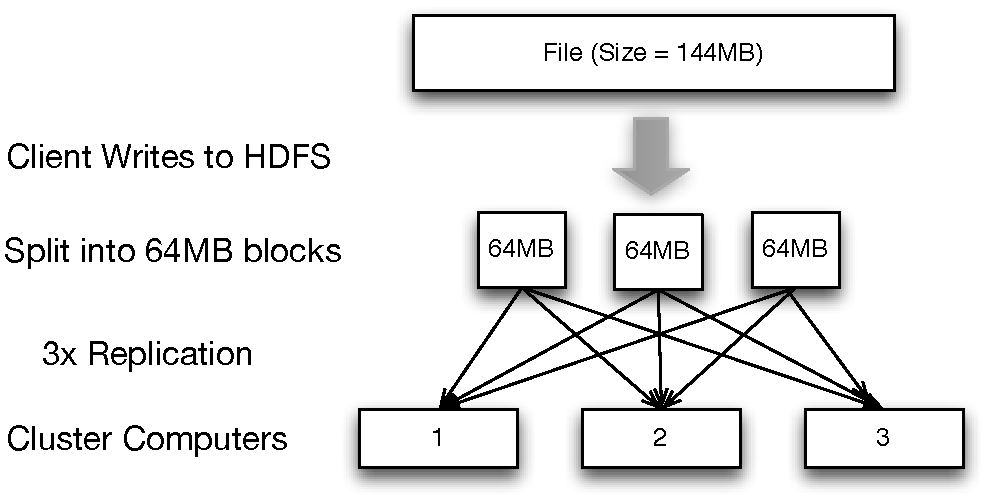
\includegraphics{hdfs-write.pdf}
\caption{A schematic of the Hadoop File System}\end{figure}


\section{Hadoop MapReduce}
\label{introduction:hadoop-mapreduce}
Concurrent programming is difficult to get right. As Herb Sutter put it:
\begin{quote}

... humans are quickly overwhelmed by concurrency and find it much more difficult to reason about concurrent than sequential code.
\end{quote}

A statistician attempting concurrent programming needs to be aware of race
conditions, deadlocks and tools to prevent this: locks, semaphores, and
mutually exclusive regions etc. An approach suggested by Sutter et al (\hyperref[introduction:stla]{{[}STLa{]}}) is to
provide programming models not functions that force
the programmer to approach her algorithms differently. Once the programmer
constructs the algorithm using this model, concurrency comes for free.  The
MapReduce programming model is one example. Correctly coded Condor DAGS are another
example.

MapReduce (\hyperref[introduction:mapred]{{[}MapRed{]}}) consists of several embarrassingly parallel splits which are evaluated
in parallel. This is called the Map. There is a synchronization guard where
intermediate data created at the end of the Map is exchanged between nodes and
another round of parallel computing starts, called the Reduce phase. In effect
large scale simulation trials in which the programmer launches several thousands
of independent computations is an example of a Map. Retrieving and collating the
results (usually done in the R console) is an example of a manual reduce.

In detail, the input to a MapReduce computation is a set of \emph{N} \emph{key,value}
pairs. The \emph{N} pairs are partitioned into \emph{S} arbitrary \emph{splits}. Each split is
a unit of computation and is assigned to one computing unit on the cluster. Thus
the processing of the \emph{S} splits occurs in parallel. Each split is processed by
a user given function \emph{M}, that takes a sequence of input key,value pairs and outputs
(one or many) intermediate key,value pairs. The Hadoop framework will partition
the intermediate values by the intermediate key. That is intermediate values
sharing the same intermediate key are grouped together. Once the map is
complete, the if there are \emph{M} distinct intermediate keys, a user given function
\emph{R}, will be given an intermediate key and all intermediate values associated
with the same key. Each processing core is assigned a subset of intermediate
keys to reduce and the reduction of the \emph{M} intermediate keys occurs in
parallel. The function \emph{R}, takes an intermediate key, a stream of associated
intermediate values and returns a final key,value pair or pairs.

The R programmer has used MapReduce ideas. For example, the \code{tapply} command
splits a vector by a list of factors. This the map equivalent: each row of the
vector is the value and the keys are the distinct levels of the list of
factors. The reduce is the user given function applied to the partitions of the
vector. The \code{xyplot} function in \code{lattice} takes a formula e.g. $F\sim
Y|A*B$, subsets the the data frame by the cartesian product of the levels of
$A$ and $B$ (the map) and displays each subset (the reduce). Hadoop
MapReduce generalizes this to a distributed level.
\begin{figure}[htbp]
\centering

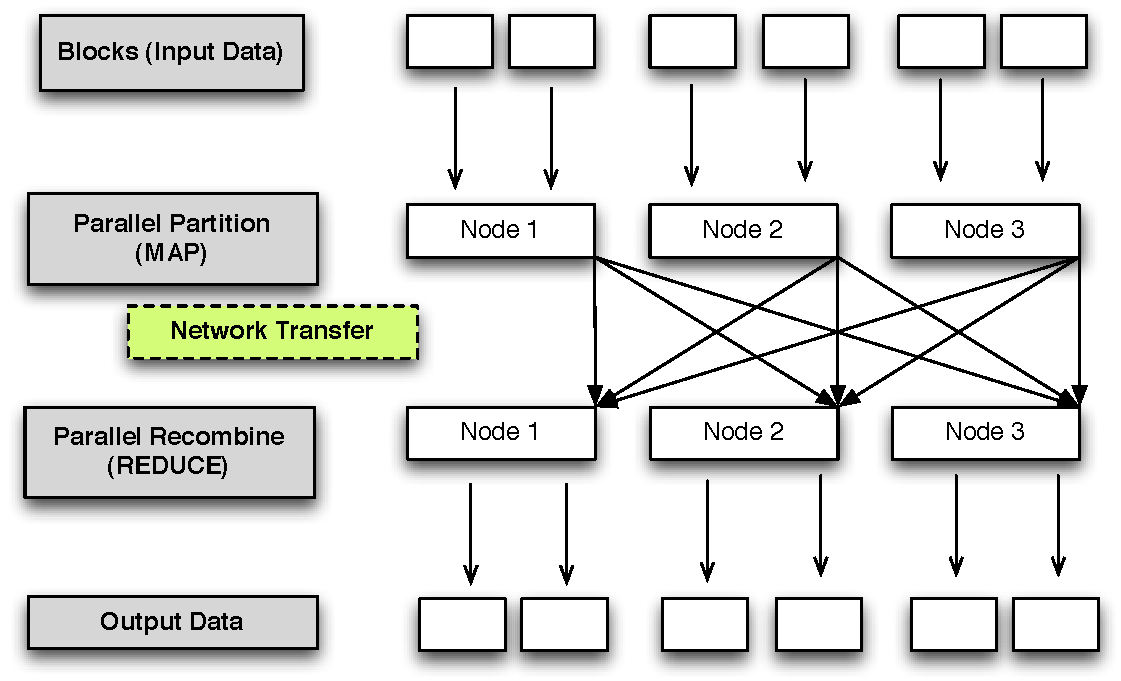
\includegraphics{mapredslov.pdf}
\caption{An overview of Hadoop MapReduce}\end{figure}


\subsection{Examples}
\label{introduction:examples}
Two examples, one for quantiles and another for correlation will be described.


\subsubsection{Approximate Quantile}
\label{introduction:approximate-quantile}\index{quantile}
Let $X$ be a column of numbers. This can be arbitrarily large
(e.g. hundreds of gigabytes). The objective is to find the quantiles of the
$X$. Let each number be a key. For discrete data e.g. ages (rounded to
years), count data, the number of unique numbers in a data set is generally not
large. For continuous data it can be many billions. In this case, we need to
discretize this. Care is needed before discretization. Discretions is equivalent
to binning and reduces the number of unique data points. For example, do not
round to the 5'th decimal place if the data points are the same for the first 5
decimal places!

For this example, let us assume the data is discrete (so no need for
rounding). The goal is to compute the frequency table of the data and use that
to compute the quantiles (see \hyperref[introduction:hynfan]{{[}HynFan{]}})

\begin{Verbatim}[commandchars=\\\{\}]
for line in line\PYGZus{}of\PYGZus{}numbers:
   for number in tokenize line by \PYG{p}{[}\PYG{p}{[}:space:\PYG{p}{]}\PYG{p}{]}:
      write\PYGZus{}key\PYGZus{}value\PYG{p}{(}number\PYG{p}{,}\PYG{l+m}{1}\PYG{p}{)}
\end{Verbatim}

The input data is partitioned into a splits of many lines of numbers. The above
code is applied to these splits in parallel. The intermediate keys are the
unique numbers and each has a list of \emph{1}`s associated with it. Hadoop will sort
the keys by the number (not neccassirly by the quantity of the number, it
depends on the programming framework) and assign the aggregation computation of
the associated values for the different unique keys to different processing
cores in the reduce phase. The reduce logic is as

\begin{Verbatim}[commandchars=\\\{\},numbers=left,firstnumber=1,stepnumber=1]
for number in stream\PYGZus{}of\PYGZus{}unique\PYGZus{}numbers:
  sum\PYG{o}{=}\PYG{l+m}{0}
  while has\PYGZus{}more\PYGZus{}values?\PYG{p}{(}\PYG{p}{)}\PYG{o}{==}\PYG{k+kc}{TRUE}:
    sum\PYG{o}{=}sum\PYG{o}{+}get\PYGZus{}new\PYGZus{}value\PYG{p}{(}\PYG{p}{)}
  end while
  write\PYGZus{}key\PYGZus{}value\PYG{p}{(}number\PYG{p}{,} sum\PYG{p}{)}
\end{Verbatim}

Notice the intermediate keys (the value of the number) and the final key (see
last line above) are the same. The unique numbers are partitioned. Thus the
stream in line 1 is stream of a subset. The different subsets are processed on
different compute cores. Note, the reduce code sums the \emph{1}`s in a \emph{while} loop
rather than loading them all into one gigantic array and adding the array. There
can be too many \emph{1}`s to fit into core. This where the MapReduce implementation
shines: big data. The algorithm finally outputs the distinct numbers of
$X$ and the counts. This can be sorted and used to compute the
quantiles. This algorithm is also used to compute word frequencies for text
document analysis.


\subsubsection{Correlation}
\label{introduction:correlation}\index{correlation}
To compute the correlation of a text file of \emph{N} rows and \emph{C} columns, we need the
sum, sums of squares of each column and sum of unique pairs of columns. The
intermediate keys and final keys are the same: the column and column pair
identifiers. The value will be the sum of columns, their sum of squares,the
cross products and the number of entries.

We need to iterate over lines, tokenize, and compute the relevant column sums
and pairwise cross products.

\begin{Verbatim}[commandchars=\\\{\},numbers=left,firstnumber=1,stepnumber=1]
for text\PYGZus{}line in stream\PYGZus{}of\PYGZus{}text\PYGZus{}lines
   tokenized\PYGZus{}line \PYG{o}{=} tokenize text\PYGZus{}line by \PYG{p}{[}\PYG{p}{[}:space:\PYG{p}{]}\PYG{p}{]}
   for i\PYG{o}{=}\PYG{l+m}{1} to C:
      rhcollect\PYG{p}{(} \PYG{p}{(}i\PYG{p}{,}i\PYG{p}{)}\PYG{p}{,} \PYG{p}{(}n\PYG{o}{=}\PYG{l+m}{1}\PYG{p}{,}sum\PYG{o}{=}tokenized\PYGZus{}line\PYG{p}{[}i\PYG{p}{]}\PYG{p}{,}ssq\PYG{o}{=}tokenized\PYGZus{}line\PYG{p}{[}i\PYG{p}{]}\PYG{o}{\PYGZca{}}\PYG{l+m}{2}\PYG{p}{)}\PYG{p}{)}
      for j\PYG{o}{=}i\PYG{o}{+}\PYG{l+m}{1} to C:
          rhcollect\PYG{p}{(} \PYG{p}{(}i\PYG{p}{,}j\PYG{p}{)}\PYG{p}{,} \PYG{p}{(}crossprod\PYG{o}{=}
                           tokenized\PYGZus{}line\PYG{p}{[}i\PYG{p}{]}\PYG{o}{*} tokenized\PYGZus{}line\PYG{p}{[}j\PYG{p}{]}\PYG{p}{)}\PYG{p}{)}
      end for
    end for
end for
\end{Verbatim}

The intermediate keys produced at the end of the map nodes are pairs
$(i,j)$ where $1 \le i \le C, i \le j\le C$ . The values are the
original value (the value for row \emph{i} and column \emph{j}), its square and
crossproduct. The \emph{n} is just a \emph{1}. By adding the values for this we obtain the
total number of rows. Inserting this \emph{1} is wasteful, since it is redundantly
being passed around for all the keys - we could compute the number of rows in
another MapReduce job.

We need to sum this:

\begin{Verbatim}[commandchars=\\\{\},numbers=left,firstnumber=1,stepnumber=1]
for identifier in stream\PYGZus{}of\PYGZus{}identifiers:
    \PYG{c+c1}{\#\# identifier is a colum pair}
    sum \PYG{o}{=} empty tuple
    while has\PYGZus{}more\PYGZus{}values?\PYG{p}{(}\PYG{p}{)}\PYG{o}{==}\PYG{k+kc}{TRUE}:
        sum \PYG{o}{=} sum \PYG{o}{+} get\PYGZus{}new\PYGZus{}value\PYG{p}{(}\PYG{p}{)}
        \PYG{c+c1}{\# get\PYGZus{}new\PYGZus{}value() will return}
        \PYG{c+c1}{\# a tuple of length}
        \PYG{c+c1}{\#     = 3 (if identifier is (i,i)}
        \PYG{c+c1}{\#     = 1 (if identifier is (i,j) i \textless{}\textgreater{} j}
    end while
    rhcollect\PYG{p}{(}identifier\PYG{p}{,} sum\PYG{p}{)}
\end{Verbatim}

The output will be a set of pairs or triplets according as the key is
$(i,i)$ or $(i,j)$.


\subsubsection{Computing an Inner Join}
\label{introduction:computing-an-inner-join}\index{inner join}
We have a text file \textbf{A} of \emph{N} columns and \textbf{B} with \emph{M} columns. Both have a
common column \textbf{index}. In \textbf{A}, it is unique, with one row per level of
\textbf{index}. \textbf{B} is a repeated measurement data set, with the levels of
\textbf{index} repeated many times. \textbf{B} also contains a column called \textbf{weight}.
We need to compute the following operation, for every unique value of \textbf{index}
in \textbf{A}, compute the mean value of \textbf{weight}. We need to join the two data
sets on \textbf{index} and compute the number of observations and sum of \textbf{weight}
for unique values \textbf{index} and save a data set which consist of only those
values of \textbf{index} found in \textbf{A}.

In SQL, this is

\begin{Verbatim}[commandchars=\\\{\}]
\PYG{k}{select}
       \PYG{k}{index}\PYG{p}{,}
       \PYG{n}{mean}\PYG{p}{(}\PYG{n}{weight}\PYG{p}{)} \PYG{k}{as} \PYG{n}{mweight}
\PYG{k}{from} \PYG{n}{A} \PYG{k}{inner} \PYG{k}{join} \PYG{n}{B}
\PYG{k}{on} \PYG{n}{A}\PYG{p}{.}\PYG{k}{index}\PYG{o}{=}\PYG{n}{B}\PYG{p}{.}\PYG{k}{index}
\PYG{k}{group} \PYG{k}{by} \PYG{n}{A}\PYG{p}{.}\PYG{k}{index}
\end{Verbatim}

1. Compute the number of observations and sum of weights aggregated by levels of
\textbf{index} for \textbf{B}. This computes the values for all levels of \textbf{index} in \textbf{B} not just those found in \textbf{A}. Call this computed data set \textbf{B'}

2. Merge \textbf{B'} and \textbf{A} .This might be wasteful since we compute for all levels in \textbf{B}, however if the
summarized data set \textbf{B'} will be used often, then this is a one time cost.

Summarizing \textbf{B} to \textbf{B'}

\begin{Verbatim}[commandchars=\\\{\},numbers=left,firstnumber=1,stepnumber=1]
\PYG{c+c1}{\#map}
for line in lines:
    index  \PYG{o}{=}  get column corresponding to \PYG{l+s}{"}\PYG{l+s}{index"} from line
    weight \PYG{o}{=}  get column corresponding to \PYG{l+s}{"}\PYG{l+s}{weight"} from line
    rhcollect\PYG{p}{(}index\PYG{p}{,}\PYG{p}{(}\PYG{l+m}{1}\PYG{p}{,}weight\PYG{p}{)}\PYG{p}{)}

\PYG{c+c1}{\#reduce}
for index in stream\PYGZus{}of\PYGZus{}indices:
    \PYG{c+c1}{\#\# identifier is a colum pair}
    sum \PYG{o}{=} empty tuple
    while has\PYGZus{}more\PYGZus{}values?\PYG{p}{(}\PYG{p}{)}\PYG{o}{==}\PYG{k+kc}{TRUE}:
        sum \PYG{o}{=} sum \PYG{o}{+} get\PYGZus{}new\PYGZus{}value\PYG{p}{(}\PYG{p}{)}
    rhcollect\PYG{p}{(}index\PYG{p}{,} sum\PYG{p}{)} \PYG{c+c1}{\#total number of obs, sum of weight}
\end{Verbatim}

To merge, we map each index value found in \textbf{A} to a TRUE value and each value
found in \textbf{B'} to a tuple (number of observations and sum of weights). If a
value of \textbf{index} is found in \emph{both} there will be two intermediate values for
that value of \textbf{index}. If instead the value of \textbf{index} exists in exactly one
of \textbf{A} and \textbf{B} there will be exactly one intermediate value. If there are
two values, one is a dummy (the TRUE) and the pseudo-code retains the value
whose length is 2 (the tuple).

\begin{Verbatim}[commandchars=\\\{\},numbers=left,firstnumber=1,stepnumber=1]
for index in stream\PYGZus{}of\PYGZus{}indices:
    count \PYG{o}{=} \PYG{l+m}{0}
    information \PYG{o}{=} \PYG{k+kc}{NULL}
    while has\PYGZus{}more\PYGZus{}values?\PYG{p}{(}\PYG{p}{)}\PYG{o}{==}\PYG{k+kc}{TRUE}:
        count \PYG{o}{=} count \PYG{o}{+} \PYG{l+m}{1}
        temp \PYG{o}{=} get\PYGZus{}next\PYGZus{}value\PYG{p}{(}\PYG{p}{)}
        if length of temp \PYG{o}{==} \PYG{l+m}{2}:
            information \PYG{o}{=} temp
    end while
    if count \PYG{o}{==} \PYG{l+m}{2}:
        rhcollect\PYG{p}{(}index\PYG{p}{,} information\PYG{p}{)}
\end{Verbatim}


\subsection{Combiners : An Optimization}
\label{introduction:combiners-an-optimization}\index{combiner}
The Hadoop framework, sends all the intermediate values for a given key to the
reducer. The intermediate values for a given key are located on several compute
nodes and need to be shuffled (sent across the network) to the node assigned the
processing of that intermediate key. This involves a lot of network
transfer. Some operations do not need access to all of the data (intermediate
values) i.e they can compute on subsets and order does not matter i.e
associative and commutative operations. For example, the minimum of 8 numbers
$min(x_1,x_2,\ldots,x_n) = min( min(x_1,x_2),min(x_3,\ldots,x_5),
min(x_6,\ldots,x_8))$

The reduction occurs on just after the map phase on a subset of intermediate
values for a given intermediate keys. The output of this is sent to the
reducer. This greatly reduces network transfer and accelerates the job speed.
\begin{figure}[htbp]
\centering

\scalebox{0.750000}{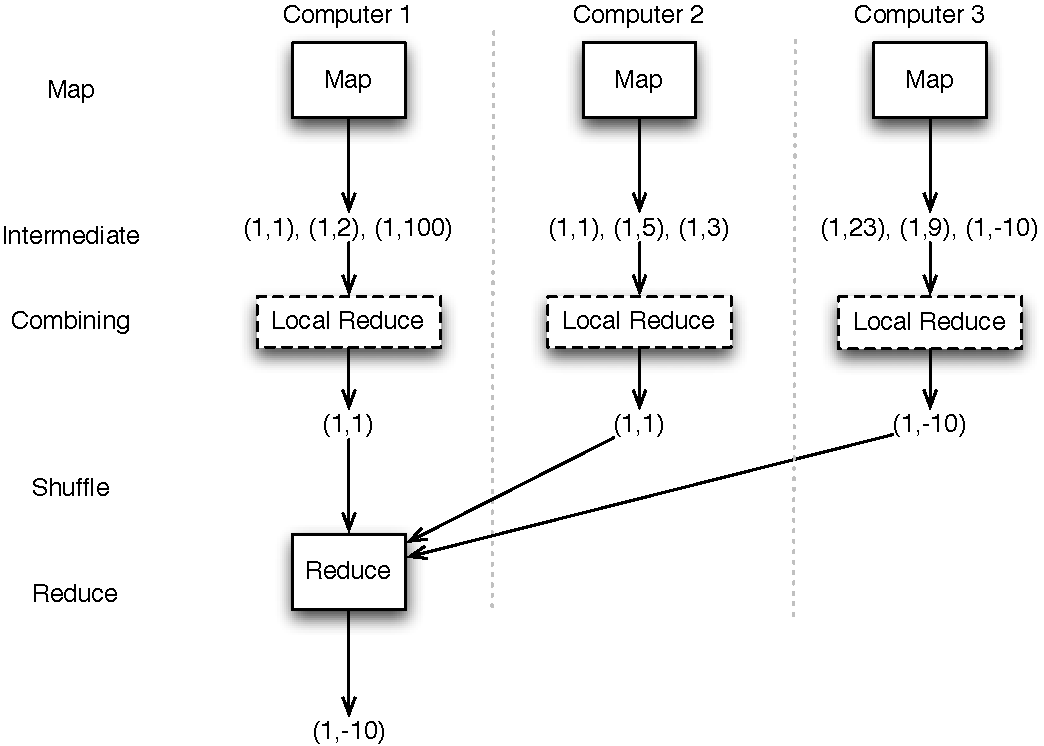
\includegraphics{combiner.pdf}}
\caption{A MapReduce job using a combiner (the minimum operator). We consider   intermediate values for a single key.}\end{figure}

The examples in this section outlined some algorithms that work with
MapReduce. Using RHIPE, there are ways to optimize the above code e.g. instead
of processing one line at a time use vector operations. Also, RHIPE calls the
code with R lists containing the input the keys and values. The streams in the
Reduce are replaced by lists of intermediate values and the R code is called
repeatedly with the list filled with new elements. This will be explained in the
Airline data example (see \emph{Airline Dataset})


\section{R and Hadoop Integrated Programming Environment}
\label{introduction:r-and-hadoop-integrated-programming-environment}
The R and Hadoop Integrated Programming Environment is R package to compute
across massive data sets, create subsets, apply routines to subsets, produce
displays on subsets across a cluster of computers using the Hadoop DFS and
Hadoop MapReduce framework. This is accomplished from within the R environment,
using standard R programming idioms. For efficiency reasons, the programming
style is slightly different from that outlined in the previous section.

The native language of Hadoop is Java. Java is not suitable for rapid
development such as is needed for a data analysis environment. \href{http://hadoop.apache.org/common/docs/current/streaming.html}{Hadoop Streaming}
bridges this gap. Users can write MapReduce programs in other languages
e.g. Python, Ruby, Perl which is then deployed over the cluster. Hadoop
Streaming then transfers the input data from Hadoop to the user program and vice
versa.

Data analysis from R does not involve the user writing code to be deployed from
the command line. The analyst has massive data sitting in the background, she
needs to create data, partition the data, compute summaries or displays. This
need to be evaluated from the R environment and the results returned to
R. Ideally not having to resort to the command line.

RHIPE is just that.
\begin{itemize}
\item {} 
RHIPE consist of several functions to interact with the HDFS e.g. save data
sets, read data created by RHIPE MapReduce, delete files.

\item {} 
Compose and launch MapReduce jobs from R using the command \code{rhmr} and
\code{rhex}. Monitor the status using \code{rhstatus} which returns an R
object. Stop jobs using \code{rhkill}

\item {} 
Compute \emph{side effect} files. The output of parallel computations may include
the creation of PDF files, R data sets, CVS files etc. These will be copied by
RHIPE to a central location on the HDFS removing the need for the user to copy
them from the compute nodes or setting up a network file system.

\item {} 
Data sets that are created by RHIPE can be read using other languages such as
Java, Perl, Python and C. The serialization format used by RHIPE (converting R
objects to binary data) uses Googles \href{http://code.google.com/p/protobuf/}{Protocol Buffers} which is very fast and creates compact
representations for R objects. Ideal for massive data sets.

\item {} 
Data sets created using RHIPE are \emph{key-value} pairs. A key is mapped to a
value. A MapReduce computations iterates over the key,value pairs in
parallel. If the output of a RHIPE job creates unique keys the output can be
treated as a external-memory associative dictionary. RHIPE can thus be used as
a medium scale (millions of keys) disk based dictionary, which is useful for
loading R objects into R.

\end{itemize}
\index{hbase}
\textbf{Future Work}
\begin{quote}

I plan on incorporating input and output bridges between RHIPE and
HBase.
\end{quote}

In summary, the objective of RHIPE is to let the user focus on thinking about
the data. The difficulties in distributing computations and storing data across
a cluster are automatically handled by RHIPE and Hadoop.


\chapter{Airline Dataset}
\label{airline:airline-dataset}\label{airline::doc}\index{airline data}
The Airline data set consists of flight arrival and departure details for all
commercial flights from 1987 to 2008. The approximately 120MM records (CSV format),  occupy
120GB space. The data set was used for the Visualization Poster Competition, JSM
2009. The winning entries can be found \href{http://stat-computing.org/dataexpo/2009/}{here} .
To quote the objectives
\begin{quote}

``The aim of the data expo is to provide a graphical summary of important
features of the data set. This is intentionally vague in order to allow
different entries to focus on different aspects of the data, but here are a
few ideas to get you started:
\begin{itemize}
\item {} 
When is the best time of day/day of week/time of year to fly to minimise delays?

\item {} 
Do older planes suffer more delays?

\item {} 
How does the number of people flying between different locations change over time?

\item {} 
How well does weather predict plane delays?

\item {} 
Can you detect cascading failures as delays in one airport create delays in
others? Are there critical links in the system?''

\end{itemize}
\end{quote}

In this chapter, I will demonstrate RHIPE code samples to create similar
graphics found in the winning entries \hyperref[airline:sas]{{[}SAS{]}} and \hyperref[airline:flusa]{{[}FLUSA{]}}


\section{Copying the Data to the HDFS (or a \emph{Distributed Downloader}!)}
\label{airline:copying-the-data-to-the-hdfs-or-a-distributed-downloader}\index{rhmr}\index{rhcounter}\index{rhstatus}\index{map.values}\index{map.keys}\index{rhex}\index{mapred.task.timeout}\index{rhstatus}\index{rhcounter}\indexiii{copying side effect files}{side effect files}{copyFiles}\phantomsection\label{airline:downloading-airline-data}
The Airline data can be found \href{http://stat-computing.org/dataexpo/2009/the-data.html}{at this site} .
In this example, we download the data sets for the individual years and save
them on the HDFS with the following code (with limited error checks)

\begin{Verbatim}[commandchars=\\\{\},numbers=left,firstnumber=1,stepnumber=1]
library\PYG{p}{(}Rhipe\PYG{p}{)}
map \PYG{o}{\textless{}-} expression\PYG{p}{(}\PYG{p}{\PYGZob{}}
  msys \PYG{o}{\textless{}-} \PYG{k+kr}{function}\PYG{p}{(}on\PYG{p}{)}\PYG{p}{\PYGZob{}}
    system\PYG{p}{(}sprintf\PYG{p}{(}\PYG{l+s}{"}\PYG{l+s}{wget  \%s --directory-prefix ./tmp 2\textgreater{} ./errors"}\PYG{p}{,}on\PYG{p}{)}\PYG{p}{)}
    \PYG{k+kr}{if}\PYG{p}{(}length\PYG{p}{(}grep\PYG{p}{(}\PYG{l+s}{"}\PYG{l+s}{(failed)\textbar{}(unable)"}\PYG{p}{,}readLines\PYG{p}{(}\PYG{l+s}{"}\PYG{l+s}{./errors"}\PYG{p}{)}\PYG{p}{)}\PYG{p}{)}\PYG{o}{\textgreater{}}\PYG{l+m}{0}\PYG{p}{)}\PYG{p}{\PYGZob{}}
      stop\PYG{p}{(}paste\PYG{p}{(}readLines\PYG{p}{(}\PYG{l+s}{"}\PYG{l+s}{./errors"}\PYG{p}{)}\PYG{p}{,}collapse\PYG{o}{=}\PYG{l+s}{"}\PYG{l+s}{\PYGZbs{}n"}\PYG{p}{)}\PYG{p}{)}
    \PYG{p}{\PYGZcb{}}\PYG{p}{\PYGZcb{}}

  lapply\PYG{p}{(}map.values\PYG{p}{,}\PYG{k+kr}{function}\PYG{p}{(}x\PYG{p}{)}\PYG{p}{\PYGZob{}}
    x\PYG{o}{=}\PYG{l+m}{1986}\PYG{o}{+}x
    on \PYG{o}{\textless{}-} sprintf\PYG{p}{(}\PYG{l+s}{"}\PYG{l+s}{http://stat-computing.org/dataexpo/2009/\%s.csv.bz2"}\PYG{p}{,}x\PYG{p}{)}
    fn \PYG{o}{\textless{}-} sprintf\PYG{p}{(}\PYG{l+s}{"}\PYG{l+s}{./tmp/\%s.csv.bz2"}\PYG{p}{,}x\PYG{p}{)}
    rhstatus\PYG{p}{(}sprintf\PYG{p}{(}\PYG{l+s}{"}\PYG{l+s}{Downloading \%s"}\PYG{p}{,} on\PYG{p}{)}\PYG{p}{)}
    msys\PYG{p}{(}on\PYG{p}{)}
    rhstatus\PYG{p}{(}sprintf\PYG{p}{(}\PYG{l+s}{"}\PYG{l+s}{Downloaded \%s"}\PYG{p}{,} on\PYG{p}{)}\PYG{p}{)}
    system\PYG{p}{(}sprintf\PYG{p}{(}\PYG{l+s}{'}\PYG{l+s}{bunzip2 \%s'}\PYG{p}{,}fn\PYG{p}{)}\PYG{p}{)}
    rhstatus\PYG{p}{(}sprintf\PYG{p}{(}\PYG{l+s}{"}\PYG{l+s}{Unzipped \%s"}\PYG{p}{,} on\PYG{p}{)}\PYG{p}{)}
    rhcounter\PYG{p}{(}\PYG{l+s}{"}\PYG{l+s}{FILES"}\PYG{p}{,}x\PYG{p}{,}\PYG{l+m}{1}\PYG{p}{)}
    rhcounter\PYG{p}{(}\PYG{l+s}{"}\PYG{l+s}{FILES"}\PYG{p}{,}\PYG{l+s}{"}\PYG{l+s}{\PYGZus{}ALL\PYGZus{}"}\PYG{p}{,}\PYG{l+m}{1}\PYG{p}{)}
  \PYG{p}{\PYGZcb{}}\PYG{p}{)}
\PYG{p}{\PYGZcb{}}\PYG{p}{)}
z \PYG{o}{\textless{}-} rhmr\PYG{p}{(}map\PYG{o}{=}map\PYG{p}{,}ofolder\PYG{o}{=}\PYG{l+s}{"}\PYG{l+s}{/airline/data"}\PYG{p}{,}inout\PYG{o}{=}c\PYG{p}{(}\PYG{l+s}{"}\PYG{l+s}{lapply"}\PYG{p}{)}\PYG{p}{,} N\PYG{o}{=}length\PYG{p}{(}\PYG{l+m}{1987}:\PYG{l+m}{2008}\PYG{p}{)}\PYG{p}{,}
          mapred\PYG{o}{=}list\PYG{p}{(}mapred.reduce.tasks\PYG{o}{=}\PYG{l+m}{0}\PYG{p}{,}mapred.task.timeout\PYG{o}{=}\PYG{l+m}{0}\PYG{p}{)}\PYG{p}{,}copyFiles\PYG{o}{=}\PYG{k+kc}{TRUE}\PYG{p}{)}
j \PYG{o}{\textless{}-} rhex\PYG{p}{(}z\PYG{p}{,}async\PYG{o}{=}\PYG{k+kc}{TRUE}\PYG{p}{)}
\end{Verbatim}

A lot is demonstrated in this code. RHIPE is loaded via the call in line 1. A
MapReduce job takes a set of input keys, in this case the numbers 1987
to 2008. It also takes a corresponding set of values. The parameter \code{inout} in
line 22 tells RHIPE how to convert the input the data to key, value pairs. If
the input file is a binary file but \code{inout} specifies \emph{text} as the input,
RHIPE will not throw an error but provide very unexpected key,value
pairs. \code{inout} in this case is \emph{lapply}, which treats the numbers 1 to \code{N}
(in line 22) as both keys and values.

These \emph{N} key,value pairs are partitioned into \emph{splits}. How they are
partitioned depends on the value of \code{inout{[}1{]}}. For text files
(\code{inout{[}1{]}='text'}), the data is split into roughly equi-length blocks of
e.g. 128MB each. A CSV text file will have approximately equal number of lines
per block (not necessarily). RHIPE will launch R across all the compute
nodes. Each node is responsible for processing a the key,value pairs in its
assigned splits.

This processing is performed in the \code{map} argument to \code{rhmr}. The \code{map}
argument is an R expression. Hadoop will read key,value pairs, send them to
RHIPE which in turn buffers them by storing them in a R list: \emph{map.values} and
\emph{map.keys} respectively. Once the buffer is full, RHIPE calls the \code{map}
expression. The default length of \emph{map.values} (and \emph{map.keys}) is 10,000 \footnote{
This can be changed by the user, see \emph{Options For RHIPE}.
}.

In our example, N is 22. The variables \emph{map.values} and \emph{map.keys} will be lists
of numbers 1 to 22 and strings ``1'' to ``22'' respectively. The entries need not be
in the order 1 to 22.

\code{rhmr} is a call that packages the MapReduce job which is sent to Hadoop. It
takes an input folder which can contain multiple files and subfolders. All the
files will be given as input. If a particular file cannot be understood by the
input format (e.g. a text file given to \code{inout{[}1{]}='sequence'}), RHIPE will throw an error.

The expression downloads the CSV file, unzips its, and stores in the folder
\emph{tmp} located in the current directory. No copying is performed. The current
directory is a temporary directory on the local filesystem of the compute node,
\textbf{not} on the HDFS. Upon successful completion of the split, the files
stored in \emph{tmp} (of the current directory) will be copied to the output folder
specified by \code{ofolder} in the call to \code{rhmr}. Files are copied \textbf{only if}
\code{copyFiles} is set to TRUE (in line 23).

Once a file has been downloaded, we inform Hadoop of our change in status, via
\code{rhastatus}. The figure \hyperref[airline:example-of-rhstatus]{\emph{Example of rhstatus}} displays the various status of each
of the 22 splits (also called Tasks)
\phantomsection\label{airline:example-of-rhstatus}\begin{figure}[htbp]
\centering

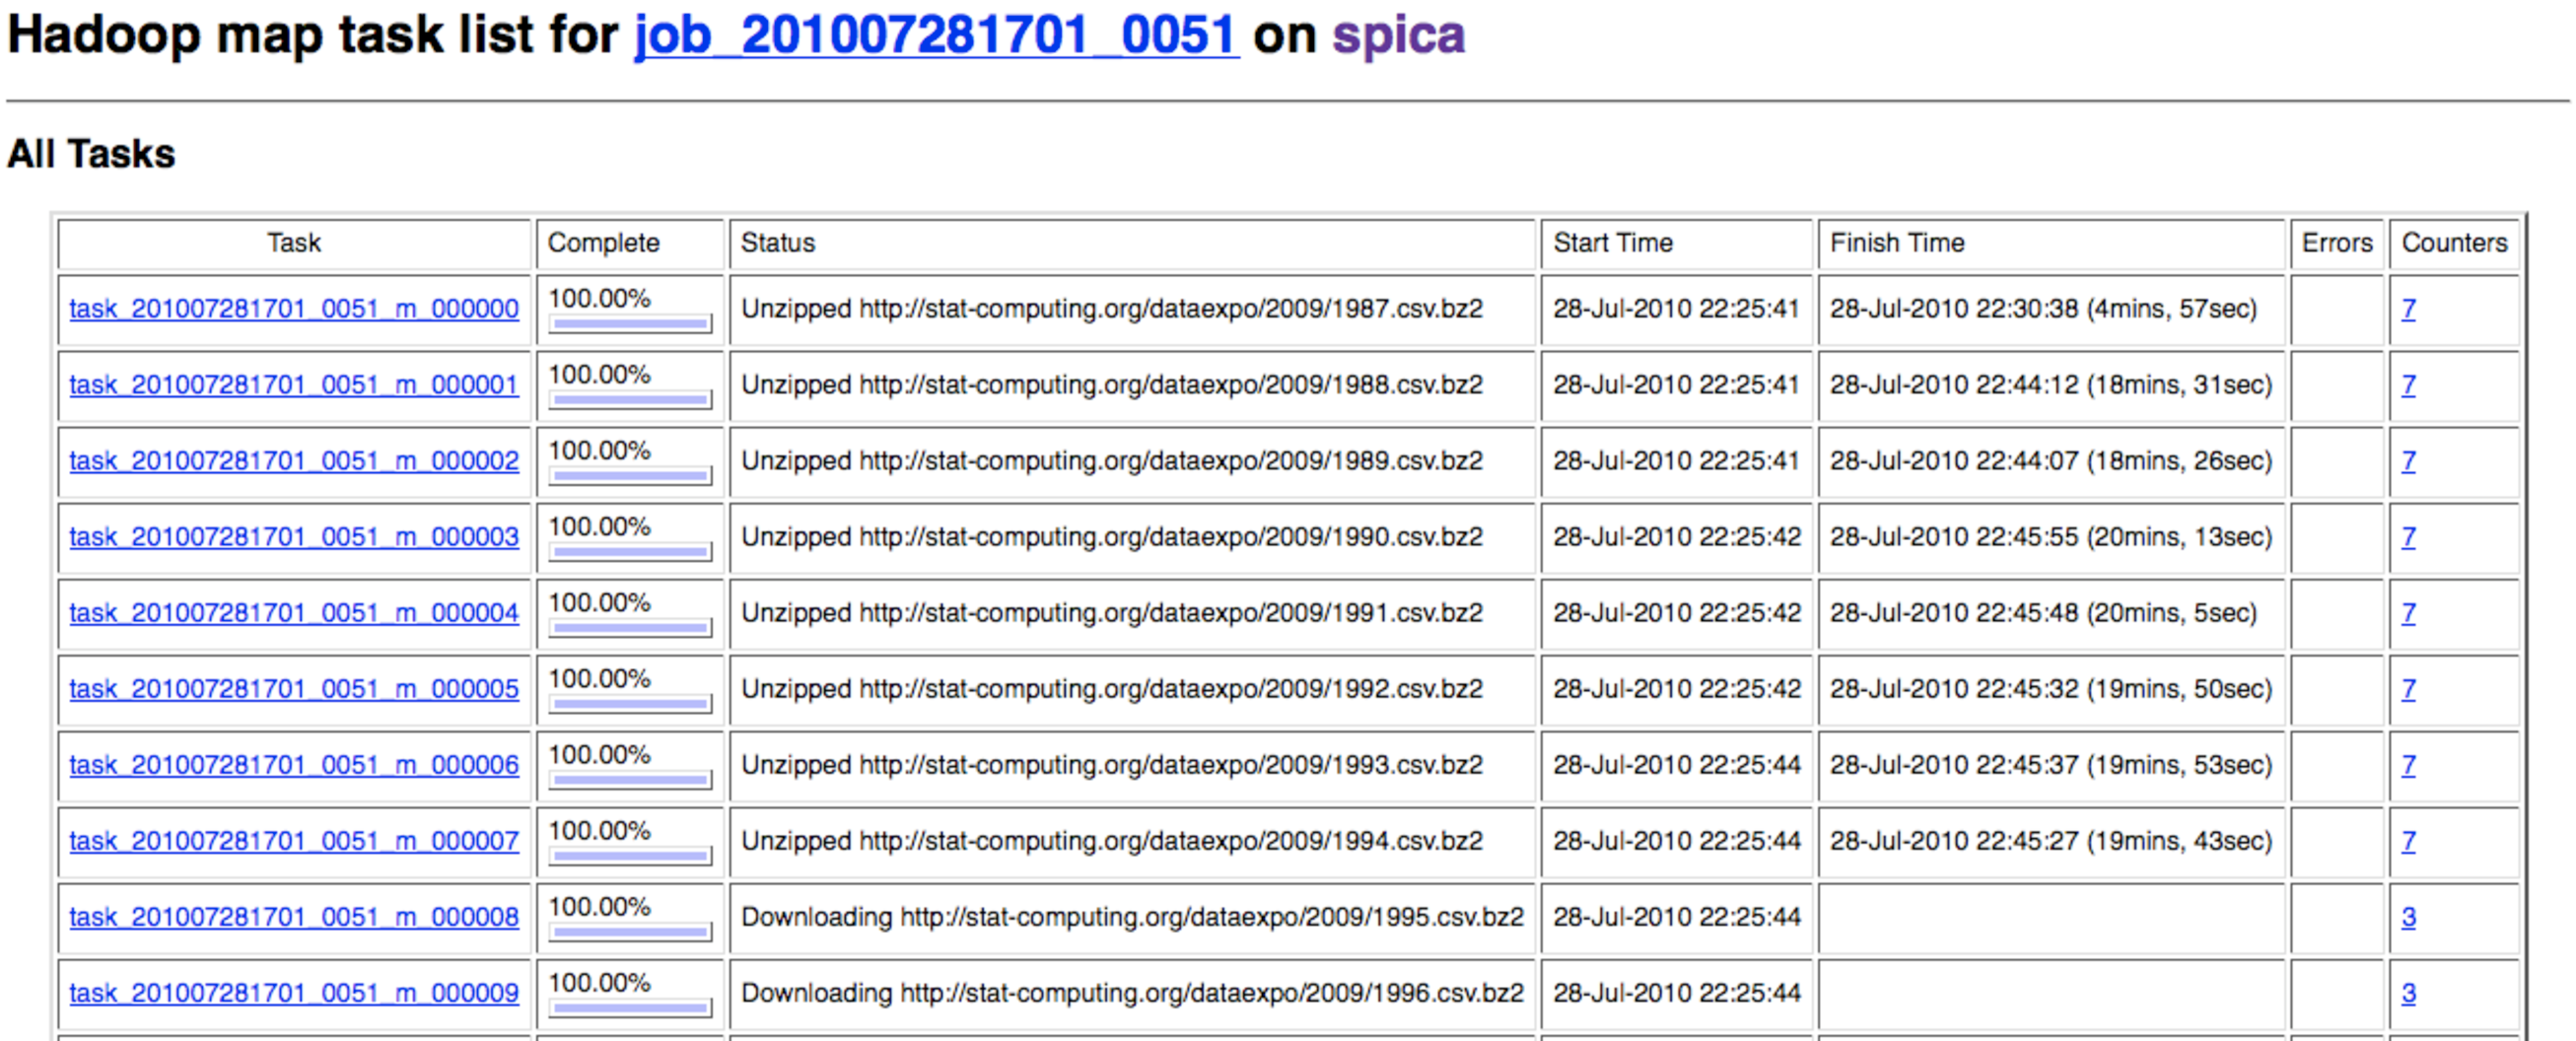
\includegraphics{rhstatus1.pdf}
\caption{Example of \code{rhstatus}}\end{figure}

Once a file has been downloaded, we increment a \textbf{distributed count}. Counts
belong to families, a single family contains many counters. The counter for
group \emph{G} and name \emph{N} is incremented via a call to \code{rhcounter}. We increment
a counter for each of the 22 files. Since each file is downloaded once, this is
essentially a flag to indicate successful download. A count of files downloaded
is tracked in \emph{Files/\_ALL\_} .

The operation of Hadoop is affected by many options, some of which can be found
in \emph{Options For RHIPE}. Hadoop will terminate splits (Tasks) after 10
minutes if they do not invoke \code{rhstatus} or return. Since each download takes
approximately 30 minutes (the minimum is 4 minutes, the maximum is 42 minutes,
the mean is 30 minutes), Hadoop will kill the tasks. We tell Hadoop to not
kill long running tasks by setting \emph{mapred.task.timeout} to 0.  We do not to
need to reduce our results so we set \emph{mapred.reduce.tasks} to 0. Output from the
map is written directly to the output folder on the HDFS. We do not have any
output. These options are passed in the \code{mapred} argument.

The call to \code{rhex} launches the job across Hadoop. We use the \code{async}
argument to return control of the R console to the user. We can monitor the
status in two ways
\index{rhstatus}\index{asynchronous execution}\begin{itemize}
\item {} 
Print the return value of \code{rhex}. The name of the job can be changed by giving a value to \code{jobname} in the
call to \code{rhmr}. The same information can be found at the Hadoop job tracker.

\end{itemize}

\begin{Verbatim}[commandchars=\\\{\},numbers=left,firstnumber=1,stepnumber=1]
\PYG{o}{\textgreater{}} j
RHIPE Job Token Information
\PYG{o}{-}\PYG{o}{-}\PYG{o}{-}\PYG{o}{-}\PYG{o}{-}\PYG{o}{-}\PYG{o}{-}\PYG{o}{-}\PYG{o}{-}\PYG{o}{-}\PYG{o}{-}\PYG{o}{-}\PYG{o}{-}\PYG{o}{-}\PYG{o}{-}\PYG{o}{-}\PYG{o}{-}\PYG{o}{-}\PYG{o}{-}\PYG{o}{-}\PYG{o}{-}\PYG{o}{-}\PYG{o}{-}\PYG{o}{-}\PYG{o}{-}\PYG{o}{-}
URL: http:\PYG{o}{/}\PYG{o}{/}spica:\PYG{l+m}{50030}\PYG{o}{/}jobdetails.jsp?jobid\PYG{o}{=}job\PYGZus{}201007281701\PYGZus{}0053
Name: \PYG{l+m}{2010}\PYG{o}{-}\PYG{l+m}{07}\PYG{o}{-}\PYG{l+m}{28} \PYG{l+m}{23}:\PYG{l+m}{33}:\PYG{l+m}{44}
ID: job\PYGZus{}201007281701\PYGZus{}0053
Submission Time: \PYG{l+m}{2010}\PYG{o}{-}\PYG{l+m}{07}\PYG{o}{-}\PYG{l+m}{28} \PYG{l+m}{23}:\PYG{l+m}{33}:\PYG{l+m}{45}
State: RUNNING
Duration\PYG{p}{(}sec\PYG{p}{)}: \PYG{l+m}{11.702}
Progess
       pct numtasks pending running complete failed
map      \PYG{l+m}{0}       \PYG{l+m}{22}       \PYG{l+m}{1}      \PYG{l+m}{21}        \PYG{l+m}{0}      \PYG{l+m}{0}
reduce   \PYG{l+m}{0}        \PYG{l+m}{0}       \PYG{l+m}{0}       \PYG{l+m}{0}        \PYG{l+m}{0}      \PYG{l+m}{0}

\PYG{o}{\textgreater{}} j
RHIPE Job Token Information
\PYG{o}{-}\PYG{o}{-}\PYG{o}{-}\PYG{o}{-}\PYG{o}{-}\PYG{o}{-}\PYG{o}{-}\PYG{o}{-}\PYG{o}{-}\PYG{o}{-}\PYG{o}{-}\PYG{o}{-}\PYG{o}{-}\PYG{o}{-}\PYG{o}{-}\PYG{o}{-}\PYG{o}{-}\PYG{o}{-}\PYG{o}{-}\PYG{o}{-}\PYG{o}{-}\PYG{o}{-}\PYG{o}{-}\PYG{o}{-}\PYG{o}{-}\PYG{o}{-}
URL: http:\PYG{o}{/}\PYG{o}{/}spica:\PYG{l+m}{50030}\PYG{o}{/}jobdetails.jsp?jobid\PYG{o}{=}job\PYGZus{}201007281701\PYGZus{}0053
Name: \PYG{l+m}{2010}\PYG{o}{-}\PYG{l+m}{07}\PYG{o}{-}\PYG{l+m}{28} \PYG{l+m}{23}:\PYG{l+m}{33}:\PYG{l+m}{44}
ID: job\PYGZus{}201007281701\PYGZus{}0053
Submission Time: \PYG{l+m}{2010}\PYG{o}{-}\PYG{l+m}{07}\PYG{o}{-}\PYG{l+m}{28} \PYG{l+m}{23}:\PYG{l+m}{33}:\PYG{l+m}{45}
State: RUNNING
Duration\PYG{p}{(}sec\PYG{p}{)}: \PYG{l+m}{56.417}
Progess
       pct numtasks pending running complete failed
map      \PYG{l+m}{1}       \PYG{l+m}{22}       \PYG{l+m}{0}      \PYG{l+m}{22}        \PYG{l+m}{0}      \PYG{l+m}{0}
reduce   \PYG{l+m}{0}        \PYG{l+m}{0}       \PYG{l+m}{0}       \PYG{l+m}{0}        \PYG{l+m}{0}      \PYG{l+m}{0}
\end{Verbatim}
\begin{itemize}
\item {} 
By calling \code{rhstatus}, giving it the value returned from \code{rhex} or the job
ID (e.g. \emph{job\_201007281701\_0053}).

\end{itemize}

\begin{Verbatim}[commandchars=\\\{\},numbers=left,firstnumber=1,stepnumber=1]
\PYG{o}{\textgreater{}} a \PYG{o}{\textless{}-} rhstatus\PYG{p}{(}j\PYG{p}{)} \PYG{c+c1}{\#\# or rhstatus("job\PYGZus{}201007281701\PYGZus{}0053")}
\PYG{o}{\textgreater{}} a\PYG{p}{\$}state
\PYG{p}{[}\PYG{l+m}{1}\PYG{p}{]} \PYG{l+s}{"}\PYG{l+s}{RUNNING"}
\PYG{o}{\textgreater{}} a\PYG{p}{\$}duration
\PYG{p}{[}\PYG{l+m}{1}\PYG{p}{]} \PYG{l+m}{902.481}
\PYG{o}{\textgreater{}} a\PYG{p}{\$}counters
\PYG{p}{\$}counters
\PYG{p}{\$}counters\PYG{p}{\$}\PYG{l+s+sb}{{}`Job Counters {}`}
Launched map tasks
                \PYG{l+m}{22}

\PYG{p}{\$}counters\PYG{p}{\$}FileSystemCounters
   FILE\PYGZus{}BYTES\PYGZus{}READ HDFS\PYGZus{}BYTES\PYGZus{}WRITTEN
         \PYG{l+m}{127162942}          \PYG{l+m}{127162942}

\PYG{p}{\$}counters\PYG{p}{\$}\PYG{l+s+sb}{{}`"FILES"{}`}
 \PYG{l+m}{1987.0} \PYG{l+s}{"}\PYG{l+s}{\PYGZus{}ALL\PYGZus{}"}
      \PYG{l+m}{1}       \PYG{l+m}{1}

\PYG{p}{\$}counters\PYG{p}{\$}\PYG{l+s+sb}{{}`Map-Reduce Framework{}`}
 Map input records    Spilled Records Map output records
                \PYG{l+m}{22}                  \PYG{l+m}{0}                  \PYG{l+m}{0}

\PYG{p}{\$}counters\PYG{p}{\$}job\PYGZus{}time
\PYG{p}{[}\PYG{l+m}{1}\PYG{p}{]} \PYG{l+m}{902.481}
\end{Verbatim}

This distributed download took 45 minutes to complete, 15 seconds more than the
longest running download (2007.csv.bz2). A sequential download would have taken
several hours.

\begin{notice}{note}{Note:}
It is important to note that the above code is mostly boiler plate. There is
almost no lines to handle distribution across a cluster or task restart in case of
transient node failure. The user of RHIPE need only consider how to frame her
argument in the concepts of MapReduce.
\end{notice}


\section{Converting to R Objects}
\label{airline:converting-to-r-objects}
The data needs to be converted to R objects. Since we will be doing repeated
analyses on the data, it is better to spend time converting them to R objects
making subsequent computations faster, rather than tokenizing strings and
converting to R objects for every analysis.

A sample of the text file

\begin{Verbatim}[commandchars=\\\{\}]
\PYG{l+m}{1987}\PYG{p}{,}\PYG{l+m}{10}\PYG{p}{,}\PYG{l+m}{23}\PYG{p}{,}\PYG{l+m}{5}\PYG{p}{,}\PYG{l+m}{1841}\PYG{p}{,}\PYG{l+m}{1750}\PYG{p}{,}\PYG{l+m}{2105}\PYG{p}{,}\PYG{l+m}{2005}\PYG{p}{,}PS\PYG{p}{,}\PYG{l+m}{1905}\PYG{p}{,}\PYG{k+kc}{NA}\PYG{p}{,}\PYG{l+m}{144}\PYG{p}{,}\PYG{l+m}{135}\PYG{p}{,}\PYG{k+kc}{NA}\PYG{p}{,}\PYG{l+m}{60}\PYG{p}{,}\PYG{l+m}{51}\PYG{p}{,}LAX\PYG{p}{,}SEA\PYG{p}{,}\PYG{l+m}{954}\PYG{p}{,}\PYG{k+kc}{NA}\PYG{p}{,}\PYG{k+kc}{NA}\PYG{p}{,}\PYG{l+m}{0}\PYG{p}{,}\PYG{k+kc}{NA}\PYG{p}{,}\PYG{l+m}{0}\PYG{p}{,}\PYG{l+m}{.}\PYG{l+m}{.}\PYG{l+m}{.}
\PYG{l+m}{1987}\PYG{p}{,}\PYG{l+m}{10}\PYG{p}{,}\PYG{l+m}{24}\PYG{p}{,}\PYG{l+m}{6}\PYG{p}{,}\PYG{l+m}{1752}\PYG{p}{,}\PYG{l+m}{1750}\PYG{p}{,}\PYG{l+m}{2010}\PYG{p}{,}\PYG{l+m}{2005}\PYG{p}{,}PS\PYG{p}{,}\PYG{l+m}{1905}\PYG{p}{,}\PYG{k+kc}{NA}\PYG{p}{,}\PYG{l+m}{138}\PYG{p}{,}\PYG{l+m}{135}\PYG{p}{,}\PYG{k+kc}{NA}\PYG{p}{,}\PYG{l+m}{5}\PYG{p}{,}\PYG{l+m}{2}\PYG{p}{,}LAX\PYG{p}{,}SEA\PYG{p}{,}\PYG{l+m}{954}\PYG{p}{,}\PYG{k+kc}{NA}\PYG{p}{,}\PYG{k+kc}{NA}\PYG{p}{,}\PYG{l+m}{0}\PYG{p}{,}\PYG{k+kc}{NA}\PYG{p}{,}\PYG{l+m}{0}\PYG{p}{,}\PYG{l+m}{.}\PYG{l+m}{.}\PYG{l+m}{.}
\PYG{l+m}{.}\PYG{l+m}{.}\PYG{l+m}{.}
\PYG{l+m}{.}\PYG{l+m}{.}\PYG{l+m}{.}
\end{Verbatim}

The meaning of the columns can be found \href{http://stat-computing.org/dataexpo/2009/the-data.html}{here} .
Rather than store the entire 120MM rows as one big data frame, it is efficient
to store it as rectangular blocks of \emph{R} rows and \emph{M} columns. We will not store
all the above columns only the following:
\begin{itemize}
\item {} 
Dates: day of week, date, month and year (1,2,3, and 4)

\item {} 
Arrival and departure times: actual and scheduled (5,6,7 and 8)

\item {} 
Flight time: actual and scheduled (12 and 13)

\item {} 
Origin and Destination: airport code, latitude and longitude (17 and 18)

\item {} 
Distance (19)

\item {} 
Carrier Name (9)

\end{itemize}

Since latitude and longitude are not present in the data sets, we will compute
them later as required. Carrier names are located in a different R data set
which will be used to do perform carrier code to carrier name translation.

We will store the data set as blocks of 5000 $\times$ 5 rows and columns. These will
be the values. Every value must be mapped to a key. In this example, the keys
(indices) to these blocks will not have any meaning but will be unique. The key
is the first scheduled departure time.
\index{sequencefile}
The format of the data is a \emph{Sequence File}, which can store binary
representations of R objects.
\index{rhmr}\index{map.keys}\index{map.values}\index{reduce.key}\index{reduce.values}
\begin{Verbatim}[commandchars=\\\{\},numbers=left,firstnumber=1,stepnumber=1]
setup \PYG{o}{\textless{}-} expression\PYG{p}{(}\PYG{p}{\PYGZob{}}
  convertHHMM \PYG{o}{\textless{}-} \PYG{k+kr}{function}\PYG{p}{(}s\PYG{p}{)}\PYG{p}{\PYGZob{}}
    t\PYG{p}{(}sapply\PYG{p}{(}s\PYG{p}{,}\PYG{k+kr}{function}\PYG{p}{(}r\PYG{p}{)}\PYG{p}{\PYGZob{}}
      l\PYG{o}{=}nchar\PYG{p}{(}r\PYG{p}{)}
      \PYG{k+kr}{if}\PYG{p}{(}l\PYG{o}{==}\PYG{l+m}{4}\PYG{p}{)} c\PYG{p}{(}substr\PYG{p}{(}r\PYG{p}{,}\PYG{l+m}{1}\PYG{p}{,}\PYG{l+m}{2}\PYG{p}{)}\PYG{p}{,}substr\PYG{p}{(}r\PYG{p}{,}\PYG{l+m}{3}\PYG{p}{,}\PYG{l+m}{4}\PYG{p}{)}\PYG{p}{)}
      \PYG{k+kr}{else} \PYG{k+kr}{if}\PYG{p}{(}l\PYG{o}{==}\PYG{l+m}{3}\PYG{p}{)} c\PYG{p}{(}substr\PYG{p}{(}r\PYG{p}{,}\PYG{l+m}{1}\PYG{p}{,}\PYG{l+m}{1}\PYG{p}{)}\PYG{p}{,}substr\PYG{p}{(}r\PYG{p}{,}\PYG{l+m}{2}\PYG{p}{,}\PYG{l+m}{3}\PYG{p}{)}\PYG{p}{)}
      \PYG{k+kr}{else} c\PYG{p}{(}\PYG{l+s}{'}\PYG{l+s}{0'}\PYG{p}{,}\PYG{l+s}{'}\PYG{l+s}{0'}\PYG{p}{)}
    \PYG{p}{\PYGZcb{}}\PYG{p}{)}
  \PYG{p}{)}\PYG{p}{\PYGZcb{}}
\PYG{p}{\PYGZcb{}}\PYG{p}{)}
map \PYG{o}{\textless{}-} expression\PYG{p}{(}\PYG{p}{\PYGZob{}}
  y \PYG{o}{\textless{}-} do.call\PYG{p}{(}\PYG{l+s}{"}\PYG{l+s}{rbind"}\PYG{p}{,}lapply\PYG{p}{(}map.values\PYG{p}{,}\PYG{k+kr}{function}\PYG{p}{(}r\PYG{p}{)}\PYG{p}{\PYGZob{}}
    \PYG{k+kr}{if}\PYG{p}{(}substr\PYG{p}{(}r\PYG{p}{,}\PYG{l+m}{1}\PYG{p}{,}\PYG{l+m}{4}\PYG{p}{)}\PYG{o}{!=}\PYG{l+s}{'}\PYG{l+s}{Year'}\PYG{p}{)} strsplit\PYG{p}{(}r\PYG{p}{,}\PYG{l+s}{"}\PYG{l+s}{,"}\PYG{p}{)}\PYG{p}{[}\PYG{p}{[}\PYG{l+m}{1}\PYG{p}{]}\PYG{p}{]}
  \PYG{p}{\PYGZcb{}}\PYG{p}{)}\PYG{p}{)}
  mu \PYG{o}{\textless{}-} rep\PYG{p}{(}\PYG{l+m}{1}\PYG{p}{,}nrow\PYG{p}{(}y\PYG{p}{)}\PYG{p}{)}\PYG{p}{;}yr \PYG{o}{\textless{}-} y\PYG{p}{[}\PYG{p}{,}\PYG{l+m}{1}\PYG{p}{]}\PYG{p}{;} mn\PYG{o}{=}y\PYG{p}{[}\PYG{p}{,}\PYG{l+m}{2}\PYG{p}{]}\PYG{p}{;}dy\PYG{o}{=}y\PYG{p}{[}\PYG{p}{,}\PYG{l+m}{3}\PYG{p}{]}
  hr \PYG{o}{\textless{}-} convertHHMM\PYG{p}{(}y\PYG{p}{[}\PYG{p}{,}\PYG{l+m}{5}\PYG{p}{]}\PYG{p}{)}
  depart \PYG{o}{\textless{}-} ISOdatetime\PYG{p}{(}year\PYG{o}{=}yr\PYG{p}{,}month\PYG{o}{=}mn\PYG{p}{,}day\PYG{o}{=}dy\PYG{p}{,}hour\PYG{o}{=}hr\PYG{p}{[}\PYG{p}{,}\PYG{l+m}{1}\PYG{p}{]}\PYG{p}{,}min\PYG{o}{=}hr\PYG{p}{[}\PYG{p}{,}\PYG{l+m}{2}\PYG{p}{]}\PYG{p}{,}sec\PYG{o}{=}mu\PYG{p}{)}
  hr \PYG{o}{\textless{}-} convertHHMM\PYG{p}{(}y\PYG{p}{[}\PYG{p}{,}\PYG{l+m}{6}\PYG{p}{]}\PYG{p}{)}
  sdepart \PYG{o}{\textless{}-} ISOdatetime\PYG{p}{(}year\PYG{o}{=}yr\PYG{p}{,}month\PYG{o}{=}mn\PYG{p}{,}day\PYG{o}{=}dy\PYG{p}{,}hour\PYG{o}{=}hr\PYG{p}{[}\PYG{p}{,}\PYG{l+m}{1}\PYG{p}{]}\PYG{p}{,}min\PYG{o}{=}hr\PYG{p}{[}\PYG{p}{,}\PYG{l+m}{2}\PYG{p}{]}\PYG{p}{,}sec\PYG{o}{=}mu\PYG{p}{)}
  hr \PYG{o}{\textless{}-} convertHHMM\PYG{p}{(}y\PYG{p}{[}\PYG{p}{,}\PYG{l+m}{7}\PYG{p}{]}\PYG{p}{)}
  arrive \PYG{o}{\textless{}-} ISOdatetime\PYG{p}{(}year\PYG{o}{=}yr\PYG{p}{,}month\PYG{o}{=}mn\PYG{p}{,}day\PYG{o}{=}dy\PYG{p}{,}hour\PYG{o}{=}hr\PYG{p}{[}\PYG{p}{,}\PYG{l+m}{1}\PYG{p}{]}\PYG{p}{,}min\PYG{o}{=}hr\PYG{p}{[}\PYG{p}{,}\PYG{l+m}{2}\PYG{p}{]}\PYG{p}{,}sec\PYG{o}{=}mu\PYG{p}{)}
  hr \PYG{o}{\textless{}-} convertHHMM\PYG{p}{(}y\PYG{p}{[}\PYG{p}{,}\PYG{l+m}{8}\PYG{p}{]}\PYG{p}{)}
  sarrive \PYG{o}{\textless{}-} ISOdatetime\PYG{p}{(}year\PYG{o}{=}yr\PYG{p}{,}month\PYG{o}{=}mn\PYG{p}{,}day\PYG{o}{=}dy\PYG{p}{,}hour\PYG{o}{=}hr\PYG{p}{[}\PYG{p}{,}\PYG{l+m}{1}\PYG{p}{]}\PYG{p}{,}min\PYG{o}{=}hr\PYG{p}{[}\PYG{p}{,}\PYG{l+m}{2}\PYG{p}{]}\PYG{p}{,}sec\PYG{o}{=}mu\PYG{p}{)}
  d \PYG{o}{\textless{}-} data.frame\PYG{p}{(}depart\PYG{o}{=} depart\PYG{p}{,}sdepart \PYG{o}{=} sdepart
                \PYG{p}{,}arrive \PYG{o}{=} arrive\PYG{p}{,}sarrive \PYG{o}{=}sarrive
                \PYG{p}{,}carrier \PYG{o}{=} y\PYG{p}{[}\PYG{p}{,}\PYG{l+m}{9}\PYG{p}{]}\PYG{p}{,}origin \PYG{o}{=} y\PYG{p}{[}\PYG{p}{,}\PYG{l+m}{17}\PYG{p}{]}
                \PYG{p}{,}dest\PYG{o}{=}y\PYG{p}{[}\PYG{p}{,}\PYG{l+m}{18}\PYG{p}{]}\PYG{p}{,}dist \PYG{o}{=} y\PYG{p}{[}\PYG{p}{,}\PYG{l+m}{19}\PYG{p}{]}\PYG{p}{,} year\PYG{o}{=}yr\PYG{p}{,} month\PYG{o}{-}mn\PYG{p}{,} day\PYG{o}{=}dy
                \PYG{p}{,}cancelled\PYG{o}{=}y\PYG{p}{[}\PYG{p}{,}\PYG{l+m}{22}\PYG{p}{]}\PYG{p}{,} stringsAsFactors\PYG{o}{=}\PYG{k+kc}{FALSE}\PYG{p}{)}
  d \PYG{o}{\textless{}-} d\PYG{p}{[}order\PYG{p}{(}d\PYG{p}{\$}sdepart\PYG{p}{)}\PYG{p}{,}\PYG{p}{]}
  rhcollect\PYG{p}{(}d\PYG{p}{[}c\PYG{p}{(}\PYG{l+m}{1}\PYG{p}{,}nrow\PYG{p}{(}d\PYG{p}{)}\PYG{p}{)}\PYG{p}{,}\PYG{l+s}{"}\PYG{l+s}{sdepart"}\PYG{p}{]}\PYG{p}{,}d\PYG{p}{)}
\PYG{p}{\PYGZcb{}}\PYG{p}{)}
reduce \PYG{o}{\textless{}-} expression\PYG{p}{(}
    reduce \PYG{o}{=} \PYG{p}{\PYGZob{}}
      lapply\PYG{p}{(}reduce.values\PYG{p}{,}\PYG{k+kr}{function}\PYG{p}{(}i\PYG{p}{)}
             rhcollect\PYG{p}{(}reduce.key\PYG{p}{,}i\PYG{p}{)}\PYG{p}{)}\PYG{p}{\PYGZcb{}}
    \PYG{p}{)}
mapred \PYG{o}{\textless{}-} list\PYG{p}{(}rhipe\PYGZus{}map\PYGZus{}buff\PYGZus{}size\PYG{o}{=}\PYG{l+m}{5000}\PYG{p}{)}
z \PYG{o}{\textless{}-} rhmr\PYG{p}{(}map\PYG{o}{=}map\PYG{p}{,}reduce\PYG{o}{=}reduce\PYG{p}{,}setup\PYG{o}{=}setup\PYG{p}{,}inout\PYG{o}{=}c\PYG{p}{(}\PYG{l+s}{"}\PYG{l+s}{text"}\PYG{p}{,}\PYG{l+s}{"}\PYG{l+s}{sequence"}\PYG{p}{)}
          \PYG{p}{,}ifolder\PYG{o}{=}\PYG{l+s}{"}\PYG{l+s}{/airline/data/"}\PYG{p}{,}ofolder\PYG{o}{=}\PYG{l+s}{"}\PYG{l+s}{/airline/blocks"}\PYG{p}{,}mapred\PYG{o}{=}mapred\PYG{p}{,}orderby\PYG{o}{=}\PYG{l+s}{"}\PYG{l+s}{numeric"}\PYG{p}{)}
rhex\PYG{p}{(}z\PYG{p}{)}
\end{Verbatim}

The \code{setup} expression is loaded into the R session \emph{once} for every
split. Remember a split can consist of many \emph{map.values} that need to be
processed. For text files as input, a split is 128MB or whatever your Hadoop
block size is. Lines 12-14, iterate over the lines and tokenizing them. The
first line in each downloaded file is the column year which must be ignored (see
line 13). The lines of text are aggregated using \code{rbind} and time related
columns converted to \emph{datetime} objects. The data frame is sorted by scheduled
departure and saved to disk indexed by the range of scheduled departures in the
data frame. The size of the value (data frame) is important. RHIPE will can
write any sized object but cannot read key,values that are more than 256MB. A
data frame of 5000 rows and 8 columns fits very well into 256MB. This is passed
to Hadoop in line 37.

Running R across massive data can be illuminating. Without the calls to
\code{ISOdatetime}, it is \textbf{much} faster to complete.
\indexii{key ordering}{ordering of keys}\index{orderby}
\textbf{Sorted keys} A reduce is not needed in this example. The text data is blocked
into data frames and written to disk. With 128MB block sizes and each block a
split, each split being mapped by one R session, there 96 files each
containing several data frames.  The reduce expression writes each incoming
intermediate value (a data frame) to disk. This is called an \emph{identity reducer}
which can be used for

1. For map file indexing. The intermediate keys are sorted. In the identity
reduce, these keys are written to disk in sorted order. If the output format
(\code{inout{[}2{]}}) is \emph{map}, the output can be used as an external memory hash
table. Given a key, RHIPE can use Hadoop to very quickly discover the location
of the key in the sorted (by key) output data and return the associated value. Thus even when no reduce logic
is required the user can provide the identity reduce to create a queryable Map
File from the map output.

2. Intermediate keys are sorted. But they can be sorted in different ways. RHIPE's
default is \emph{byte ordering} i.e the keys are serialized to bytes and sorted
byte wise. However, byte ordering is very different from semantic
ordering. Thus keys e.g. 10,-1,20 which might be byte ordered are certainly not
numerically ordered. RHIPE can numerically order keys so that in the reduce
expression the user is guaranteed to receive the keys in sorted numeric
order. In the above code, we request this feature in line 38. Numeric sorting
is as follows: keys A and B are ordered if $A<B$ and of unit length or
or $A[i]<B[i], 1\le i \le min(length(A),length(B))$ \footnote{
A similar ordering exists for character vectors (\code{NA} not.. allowed). Specify by setting \code{orderby="character"} in the call to \code{rhmr}
}.
For keys $1,(2,1),(1,1),5,(1,3,4),(2,1),4,(4,9)$ the ordering is $1,(1,1),(1,3,4),(2,1),(2,1),4,(4,9),5$
Using this ordering, all the values in a given file will be ordered by the
range of the scheduled departures.  Using this custom sorter can be slower than
the default byte ordering. Bear in mind, the keys in a \emph{part} file will be ordered but keys in one \emph{part} file need not be less than those in another \emph{part} file.
\phantomsection\label{airline:tuple-sorting}
To achieve ordering of keys set \emph{orderby} in the call to \code{rhmr} to one of
\emph{bytes} (default), \emph{integer}, \emph{numeric} (for doubles) or \emph{character}
(alphabetical sorting) in the \code{mapred} argument to \code{rhmr}. If the output
format is \emph{sequence}, you also need to provide a reducer which can be an
identity reducer. Note, if your keys are discrete, it is best to use \emph{integer} ordering. Values of NA can throw of ordering
and will send \emph{all} key,values to one reducer causing a severe imbalance.

\begin{Verbatim}[commandchars=\\\{\}]
reduce \PYG{o}{=} expression\PYG{p}{(}\PYG{p}{\PYGZob{}}
  reduce\PYG{o}{=}\PYG{p}{\PYGZob{}} lapply\PYG{p}{(}reduce.values\PYG{p}{,}\PYG{k+kr}{function}\PYG{p}{(}r\PYG{p}{)} rhcollect\PYG{p}{(}reduce.key\PYG{p}{,}r\PYG{p}{)}\PYG{p}{)} \PYG{p}{\PYGZcb{}}
\PYG{p}{\PYGZcb{}}\PYG{p}{)}
\end{Verbatim}

3. To decrease the number of files. In this case decreasing the number of files is
hardly needed, but it can be useful if one has more thousands of splits.

In situations (1) and (3), the user does not have to provide the R reduce
expression and can leave this parameter empty. In situation (2), you need to
provide the above code. Also, (2) is incompatible with Map File outputs (i.e
\code{inout{[}2{]}} set to \emph{map}). Case (2) is mostly useful for time series algorithms
in the reduce section e.g. keys of the form $(identifier,i)`$ where
\emph{identifier} is an object and \emph{i} ranges from \emph{1} to $n_{identifier}$. For
each key, the value is sorted time series data. The reducer will receive the
values for the keys $(identifier,i)`$ in the order of \emph{i} for a given
\emph{identifier}. This also assumes the user has partitioned the data on
\emph{identifier} (see the \code{part} parameter of \code{rhmr}: for this to work, all the
keys  $(identifier,i)`$ with the same \emph{identifier} need to be sent to the
same reducer). For an example see \hyperref[airline:streaming-data]{\emph{Streaming Data?}}.

A sample data frame (last 4 columns removed):

\begin{Verbatim}[commandchars=\\\{\}]
                 depart              sarrive      carrier origin dest dist cancelled
\PYG{l+m}{2880} \PYG{l+m}{1988}\PYG{o}{-}\PYG{l+m}{05}\PYG{o}{-}\PYG{l+m}{01} \PYG{l+m}{01}:\PYG{l+m}{02}:\PYG{l+m}{01} \PYG{l+m}{.}\PYG{l+m}{.}\PYG{l+m}{.} \PYG{l+m}{1988}\PYG{o}{-}\PYG{l+m}{05}\PYG{o}{-}\PYG{l+m}{01} \PYG{l+m}{01}:\PYG{l+m}{59}:\PYG{l+m}{01}      DL    SLC  SEA  \PYG{l+m}{689}         \PYG{l+m}{0}
\PYG{l+m}{3770} \PYG{l+m}{1988}\PYG{o}{-}\PYG{l+m}{05}\PYG{o}{-}\PYG{l+m}{01} \PYG{l+m}{01}:\PYG{l+m}{10}:\PYG{l+m}{01} \PYG{l+m}{.}\PYG{l+m}{.}\PYG{l+m}{.} \PYG{l+m}{1988}\PYG{o}{-}\PYG{l+m}{05}\PYG{o}{-}\PYG{l+m}{01} \PYG{l+m}{02}:\PYG{l+m}{13}:\PYG{l+m}{01}      DL    JAX  FLL  \PYG{l+m}{318}         \PYG{l+m}{0}
\PYG{l+m}{2137} \PYG{l+m}{1988}\PYG{o}{-}\PYG{l+m}{05}\PYG{o}{-}\PYG{l+m}{01} \PYG{l+m}{01}:\PYG{l+m}{10}:\PYG{l+m}{01} \PYG{l+m}{.}\PYG{l+m}{.}\PYG{l+m}{.} \PYG{l+m}{1988}\PYG{o}{-}\PYG{l+m}{05}\PYG{o}{-}\PYG{l+m}{01} \PYG{l+m}{01}:\PYG{l+m}{59}:\PYG{l+m}{01}      DL    TPA  PBI  \PYG{l+m}{174}         \PYG{l+m}{0}
\end{Verbatim}


\section{Demonstration of using Hadoop as a Queryable Database}
\label{airline:demonstration-of-using-hadoop-as-a-queryable-database}\index{rhgetkey}\index{map files}\index{rhipe\_map\_buff\_size}\index{combiner}
\emph{Sightly artificial}: store all Southwest Airlines information indexed by
year,month,and day. Each (year, month, day) triplet will have all flight entries
that left on that day. Using the above data set as the source, the Southwest
lines are selected and sent to the reducer with the (year, month,day) key. All
flights with the same (year, month) will belong to the same file. Given a (year,
month,day) triplet, we can use the Map File output format to access the
associated flight information in seconds rather than subsetting using MapReduce.

\begin{Verbatim}[commandchars=\\\{\},numbers=left,firstnumber=1,stepnumber=1]
map \PYG{o}{\textless{}-} expression\PYG{p}{(}\PYG{p}{\PYGZob{}}
  h \PYG{o}{\textless{}-} do.call\PYG{p}{(}\PYG{l+s}{"}\PYG{l+s}{rbind"}\PYG{p}{,}map.values\PYG{p}{)}
  d \PYG{o}{\textless{}-} h\PYG{p}{[}h\PYG{p}{\$}carrier\PYG{o}{==}\PYG{l+s}{'}\PYG{l+s}{WN'}\PYG{p}{,}\PYG{p}{,}drop\PYG{o}{=}\PYG{k+kc}{FALSE}\PYG{p}{]}
  \PYG{k+kr}{if}\PYG{p}{(}nrow\PYG{p}{(}d\PYG{p}{)}\PYG{o}{\textgreater{}}\PYG{l+m}{0}\PYG{p}{)}\PYG{p}{\PYGZob{}}
    e \PYG{o}{\textless{}-} split\PYG{p}{(}d\PYG{p}{,}list\PYG{p}{(}d\PYG{p}{\$}year\PYG{p}{,}d\PYG{p}{\$}month\PYG{p}{,}d\PYG{p}{\$}mday\PYG{p}{)}\PYG{p}{)}
    lapply\PYG{p}{(}e\PYG{p}{,}\PYG{k+kr}{function}\PYG{p}{(}r\PYG{p}{)}\PYG{p}{\PYGZob{}}
      k \PYG{o}{\textless{}-} as.vector\PYG{p}{(}unlist\PYG{p}{(}r\PYG{p}{[}\PYG{l+m}{1}\PYG{p}{,}c\PYG{p}{(}\PYG{l+s}{"}\PYG{l+s}{year"}\PYG{p}{,}\PYG{l+s}{"}\PYG{l+s}{month"}\PYG{p}{,}\PYG{l+s}{"}\PYG{l+s}{mday"}\PYG{p}{)}\PYG{p}{]}\PYG{p}{)}\PYG{p}{)}  \PYG{c+c1}{\#\# remove attributes}
      rhcollect\PYG{p}{(}k\PYG{p}{,} r\PYG{p}{)}
    \PYG{p}{\PYGZcb{}}\PYG{p}{)}
  \PYG{p}{\PYGZcb{}}
\PYG{p}{\PYGZcb{}}\PYG{p}{)}
reduce \PYG{o}{\textless{}-} expression\PYG{p}{(}
    pre \PYG{o}{=} \PYG{p}{\PYGZob{}} collec \PYG{o}{\textless{}-} \PYG{k+kc}{NULL} \PYG{p}{\PYGZcb{}}\PYG{p}{,}
    reduce \PYG{o}{=} \PYG{p}{\PYGZob{}}
      collec \PYG{o}{\textless{}-} rbind\PYG{p}{(}collec\PYG{p}{,} do.call\PYG{p}{(}\PYG{l+s}{"}\PYG{l+s}{rbind"}\PYG{p}{,}reduce.values\PYG{p}{)}\PYG{p}{)}
      collec \PYG{o}{\textless{}-} collec\PYG{p}{[}order\PYG{p}{(}collec\PYG{p}{\$}depart\PYG{p}{)}\PYG{p}{,}\PYG{p}{]}
    \PYG{p}{\PYGZcb{}}\PYG{p}{,}
    post \PYG{o}{=} \PYG{p}{\PYGZob{}}
      rhcollect\PYG{p}{(}k\PYG{p}{,} collec\PYG{p}{)}
    \PYG{p}{\PYGZcb{}}
    \PYG{p}{)}
z \PYG{o}{\textless{}-} rhmr\PYG{p}{(}map\PYG{o}{=}map\PYG{p}{,}reduce\PYG{o}{=}reduce\PYG{p}{,}combiner\PYG{o}{=}\PYG{k+kc}{TRUE}\PYG{p}{,}inout\PYG{o}{=}c\PYG{p}{(}\PYG{l+s}{"}\PYG{l+s}{sequence"}\PYG{p}{,}\PYG{l+s}{"}\PYG{l+s}{map"}\PYG{p}{)}
          \PYG{p}{,}ifolder\PYG{o}{=}\PYG{l+s}{"}\PYG{l+s}{/airline/blocks/"}\PYG{p}{,}ofolder\PYG{o}{=}\PYG{l+s}{"}\PYG{l+s}{/airline/southwest"}
          \PYG{p}{,}mapred\PYG{o}{=}list\PYG{p}{(}rhipe\PYGZus{}map\PYGZus{}buff\PYGZus{}size\PYG{o}{=}\PYG{l+m}{10}\PYG{p}{)}\PYG{p}{)}
rhex\PYG{p}{(}z\PYG{p}{)}
\end{Verbatim}

Attributes are removed in line 8, for otherwise we have to retrieve a data frame
with a data frame with column names and row names instead of a more convenient
numeric vector.  The map expression combines the individual data frames. Each
data frame has 5000 rows, hence \emph{rhipe\_map\_buff\_size} is set to 10 for a
combined data frame of 50000 rows in line 32. This is crucial. The default value
for \emph{rhipe\_map\_buff\_size} is 10,000. Binding 10,000 data frames of 5000 rows
each creates a data frame of 50MN rows - too unwieldy to compute with in R (for
many types of operations). Data frames for Southwest Airlines (carried code=WN)
are created and emitted with the call to \code{rhcollect} in line 15. These are
combined in the reduce since data frames for the same (year, month,day) triplet
can be emitted from different map expressions. Since this is associative and
commutative we use a combiner. The output format (\code{inout{[}{[}2{]}{]}}) is \emph{map}, so
we can access the flights for any triplet with a call to \code{rhgetkey} which
returns a list of key,value lists.

\begin{Verbatim}[commandchars=\\\{\},numbers=left,firstnumber=1,stepnumber=1]
\PYG{o}{\textgreater{}} a \PYG{o}{\textless{}-} rhgetkey\PYG{p}{(}list\PYG{p}{(}c\PYG{p}{(}\PYG{l+m}{88}\PYG{p}{,}\PYG{l+m}{2}\PYG{p}{,}\PYG{l+m}{17}\PYG{p}{)}\PYG{p}{)}\PYG{p}{,}\PYG{l+s}{"}\PYG{l+s}{/airline/southwest"}\PYG{p}{)}
\PYG{o}{\textgreater{}} a\PYG{p}{[}\PYG{p}{[}\PYG{l+m}{1}\PYG{p}{]}\PYG{p}{]}\PYG{p}{[}\PYG{p}{[}\PYG{l+m}{1}\PYG{p}{]}\PYG{p}{]}
\PYG{p}{[}\PYG{l+m}{1}\PYG{p}{]} \PYG{l+m}{93}  \PYG{l+m}{0}  \PYG{l+m}{1}
\PYG{o}{\textgreater{}} head\PYG{p}{(}a\PYG{p}{[}\PYG{p}{[}\PYG{l+m}{1}\PYG{p}{]}\PYG{p}{]}\PYG{p}{[}\PYG{p}{[}\PYG{l+m}{2}\PYG{p}{]}\PYG{p}{]}\PYG{p}{[}\PYG{p}{,}\PYG{l+m}{1}:\PYG{l+m}{9}\PYG{p}{]}\PYG{p}{)}
                    depart                 sarrive carrier origin dest dist cancelled
\PYG{l+m}{23648}  \PYG{l+m}{1993}\PYG{o}{-}\PYG{l+m}{01}\PYG{o}{-}\PYG{l+m}{01} \PYG{l+m}{00}:\PYG{l+m}{00}:\PYG{l+m}{01} \PYG{l+m}{.}\PYG{l+m}{.}\PYG{l+m}{.} \PYG{l+m}{1993}\PYG{o}{-}\PYG{l+m}{01}\PYG{o}{-}\PYG{l+m}{01} \PYG{l+m}{13}:\PYG{l+m}{35}:\PYG{l+m}{01}      WN    RNO  LAS  \PYG{l+m}{345}         \PYG{l+m}{1}
\PYG{l+m}{20714}  \PYG{l+m}{1993}\PYG{o}{-}\PYG{l+m}{01}\PYG{o}{-}\PYG{l+m}{01} \PYG{l+m}{07}:\PYG{l+m}{20}:\PYG{l+m}{01} \PYG{l+m}{.}\PYG{l+m}{.}\PYG{l+m}{.} \PYG{l+m}{1993}\PYG{o}{-}\PYG{l+m}{01}\PYG{o}{-}\PYG{l+m}{01} \PYG{l+m}{08}:\PYG{l+m}{40}:\PYG{l+m}{01}      WN    SFO  SAN  \PYG{l+m}{447}         \PYG{l+m}{0}
\PYG{l+m}{37642}  \PYG{l+m}{1993}\PYG{o}{-}\PYG{l+m}{01}\PYG{o}{-}\PYG{l+m}{01} \PYG{l+m}{07}:\PYG{l+m}{25}:\PYG{l+m}{01} \PYG{l+m}{.}\PYG{l+m}{.}\PYG{l+m}{.} \PYG{l+m}{1993}\PYG{o}{-}\PYG{l+m}{01}\PYG{o}{-}\PYG{l+m}{01} \PYG{l+m}{10}:\PYG{l+m}{15}:\PYG{l+m}{01}      WN    OAK  PHX  \PYG{l+m}{646}         \PYG{l+m}{0}
\PYG{l+m}{316110} \PYG{l+m}{1993}\PYG{o}{-}\PYG{l+m}{01}\PYG{o}{-}\PYG{l+m}{01} \PYG{l+m}{07}:\PYG{l+m}{30}:\PYG{l+m}{01} \PYG{l+m}{.}\PYG{l+m}{.}\PYG{l+m}{.} \PYG{l+m}{1993}\PYG{o}{-}\PYG{l+m}{01}\PYG{o}{-}\PYG{l+m}{01} \PYG{l+m}{08}:\PYG{l+m}{30}:\PYG{l+m}{01}      WN    OAK  BUR  \PYG{l+m}{325}         \PYG{l+m}{0}
\end{Verbatim}


\section{Analyses}
\label{airline:analyses}
We compute some summaries and displays to understand the data.


\subsection{Top 20 cities by total volume of flights.}
\label{airline:top-20-cities-by-total-volume-of-flights}
What are the busiest cities by total flight traffic. JFK will feature, but what
are the others? For each airport code compute the number of inbound, outbound
and all flights.
\index{rhmr}\index{rhex}\index{rhread}\index{rhex}
\begin{Verbatim}[commandchars=\\\{\},numbers=left,firstnumber=1,stepnumber=1]
map \PYG{o}{\textless{}-} expression\PYG{p}{(}\PYG{p}{\PYGZob{}}
  a \PYG{o}{\textless{}-} do.call\PYG{p}{(}\PYG{l+s}{"}\PYG{l+s}{rbind"}\PYG{p}{,}map.values\PYG{p}{)}
  inbound \PYG{o}{\textless{}-} table\PYG{p}{(}a\PYG{p}{[}\PYG{p}{,}\PYG{l+s}{'}\PYG{l+s}{origin'}\PYG{p}{]}\PYG{p}{)}
  outbound \PYG{o}{\textless{}-} table\PYG{p}{(}a\PYG{p}{[}\PYG{p}{,}\PYG{l+s}{'}\PYG{l+s}{dest'}\PYG{p}{]}\PYG{p}{)}
  total \PYG{o}{\textless{}-} table\PYG{p}{(}unlist\PYG{p}{(}c\PYG{p}{(}a\PYG{p}{[}\PYG{p}{,}\PYG{l+s}{'}\PYG{l+s}{origin'}\PYG{p}{]}\PYG{p}{,}a\PYG{p}{[}\PYG{l+s}{'}\PYG{l+s}{dest'}\PYG{p}{]}\PYG{p}{)}\PYG{p}{)}\PYG{p}{)}
  \PYG{k+kr}{for}\PYG{p}{(}n in names\PYG{p}{(}total\PYG{p}{)}\PYG{p}{)}\PYG{p}{\PYGZob{}}
    inb \PYG{o}{\textless{}-} \PYG{k+kr}{if}\PYG{p}{(}is.na\PYG{p}{(}inbound\PYG{p}{[}n\PYG{p}{]}\PYG{p}{)}\PYG{p}{)} \PYG{l+m}{0} \PYG{k+kr}{else} inbound\PYG{p}{[}n\PYG{p}{]}
    ob \PYG{o}{\textless{}-} \PYG{k+kr}{if}\PYG{p}{(}is.na\PYG{p}{(}outbound\PYG{p}{[}n\PYG{p}{]}\PYG{p}{)}\PYG{p}{)} \PYG{l+m}{0} \PYG{k+kr}{else} outbound\PYG{p}{[}n\PYG{p}{]}
    rhcollect\PYG{p}{(}n\PYG{p}{,} c\PYG{p}{(}inb\PYG{p}{,}ob\PYG{p}{,} total\PYG{p}{[}n\PYG{p}{]}\PYG{p}{)}\PYG{p}{)}
  \PYG{p}{\PYGZcb{}}
\PYG{p}{\PYGZcb{}}\PYG{p}{)}
reduce \PYG{o}{\textless{}-} expression\PYG{p}{(}
    pre\PYG{o}{=}\PYG{p}{\PYGZob{}}sums \PYG{o}{\textless{}-} c\PYG{p}{(}\PYG{l+m}{0}\PYG{p}{,}\PYG{l+m}{0}\PYG{p}{,}\PYG{l+m}{0}\PYG{p}{)}\PYG{p}{\PYGZcb{}}\PYG{p}{,}
    reduce \PYG{o}{=} \PYG{p}{\PYGZob{}}
      sums \PYG{o}{\textless{}-} sums\PYG{o}{+}apply\PYG{p}{(}do.call\PYG{p}{(}\PYG{l+s}{"}\PYG{l+s}{rbind"}\PYG{p}{,}reduce.values\PYG{p}{)}\PYG{p}{,}\PYG{l+m}{2}\PYG{p}{,}sum\PYG{p}{)}
    \PYG{p}{\PYGZcb{}}\PYG{p}{,}
    post \PYG{o}{=} \PYG{p}{\PYGZob{}}
      rhcollect\PYG{p}{(}reduce.key\PYG{p}{,} sums\PYG{p}{)}
    \PYG{p}{\PYGZcb{}}
    \PYG{p}{)}
mapred\PYG{p}{\$}rhipe\PYGZus{}map\PYGZus{}buff\PYGZus{}size \PYG{o}{\textless{}-} \PYG{l+m}{15}
z \PYG{o}{\textless{}-} rhmr\PYG{p}{(}map\PYG{o}{=}map\PYG{p}{,}reduce\PYG{o}{=}reduce\PYG{p}{,}combiner\PYG{o}{=}\PYG{k+kc}{TRUE}\PYG{p}{,}inout\PYG{o}{=}c\PYG{p}{(}\PYG{l+s}{"}\PYG{l+s}{sequence"}\PYG{p}{,}\PYG{l+s}{"}\PYG{l+s}{sequence"}\PYG{p}{)}
          \PYG{p}{,}ifolder\PYG{o}{=}\PYG{l+s}{"}\PYG{l+s}{/airline/blocks/"}\PYG{p}{,}ofolder\PYG{o}{=}\PYG{l+s}{"}\PYG{l+s}{/airline/volume"}
          \PYG{p}{,}mapred\PYG{o}{=}mapred\PYG{p}{)}
rhex\PYG{p}{(}z\PYG{p}{,}async\PYG{o}{=}\PYG{k+kc}{TRUE}\PYG{p}{)}
\end{Verbatim}

The code is straightforward. I increased the value of \emph{rhipe\_map\_buff\_size}
since we are doing summaries of columns. The figure \hyperref[airline:time-to-complete-vs-rhipe-map-buff-size]{\emph{Log of time to complete vs log of rhipe\_map\_buff\_size.}} plots the time of completion vs the mean of three
trials for different values of \emph{rhipe\_map\_buff\_size}. The trials set
\emph{rhipe\_map\_buff\_size} to 5,10,15,20,25 and 125. All experiments (like the rest
in the manual) were performed on a 72 core cluster across 8 servers with RAM
varying from 16 to 64 GB.
\phantomsection\label{airline:time-to-complete-vs-rhipe-map-buff-size}\begin{figure}[htbp]
\centering

\scalebox{0.500000}{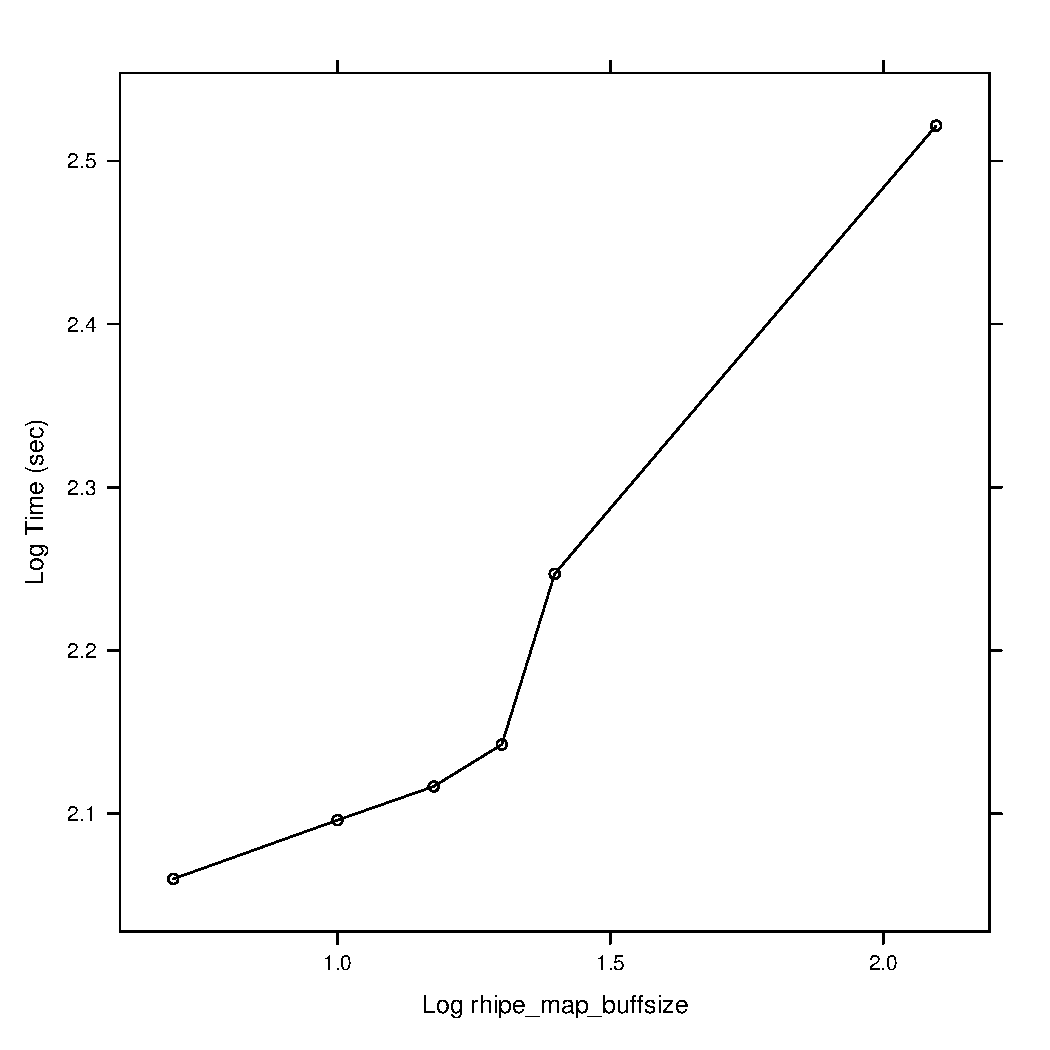
\includegraphics{rhipemapbuff.pdf}}
\caption{Log of time to complete vs log of \emph{rhipe\_map\_buff\_size}.}\end{figure}

Read the data into R and display them using the \code{lattice} library.
\index{rhread}
\begin{Verbatim}[commandchars=\\\{\},numbers=left,firstnumber=1,stepnumber=1]
counts \PYG{o}{\textless{}-} rhread\PYG{p}{(}\PYG{l+s}{"}\PYG{l+s}{/airline/volume"}\PYG{p}{)}
aircode \PYG{o}{\textless{}-} unlist\PYG{p}{(}lapply\PYG{p}{(}counts\PYG{p}{,} \PYG{l+s}{"}\PYG{l+s}{[["}\PYG{p}{,}\PYG{l+m}{1}\PYG{p}{)}\PYG{p}{)}
count \PYG{o}{\textless{}-} do.call\PYG{p}{(}\PYG{l+s}{"}\PYG{l+s}{rbind"}\PYG{p}{,}lapply\PYG{p}{(}counts\PYG{p}{,}\PYG{l+s}{"}\PYG{l+s}{[["}\PYG{p}{,}\PYG{l+m}{2}\PYG{p}{)}\PYG{p}{)}
results \PYG{o}{\textless{}-} data.frame\PYG{p}{(}aircode\PYG{o}{=}aircode\PYG{p}{,}
                      inb\PYG{o}{=}count\PYG{p}{[}\PYG{p}{,}\PYG{l+m}{1}\PYG{p}{]}\PYG{p}{,}oub\PYG{o}{=}count\PYG{p}{[}\PYG{p}{,}\PYG{l+m}{2}\PYG{p}{]}\PYG{p}{,}all\PYG{o}{=}count\PYG{p}{[}\PYG{p}{,}\PYG{l+m}{3}\PYG{p}{]}
                      \PYG{p}{,}stringsAsFactors\PYG{o}{=}\PYG{k+kc}{FALSE}\PYG{p}{)}
results \PYG{o}{\textless{}-} results\PYG{p}{[}order\PYG{p}{(}results\PYG{p}{\$}all\PYG{p}{,}decreasing\PYG{o}{=}\PYG{k+kc}{TRUE}\PYG{p}{)}\PYG{p}{,}\PYG{p}{]}
results\PYG{p}{\$}airport \PYG{o}{\textless{}-} sapply\PYG{p}{(}results\PYG{p}{\$}aircode\PYG{p}{,}\PYG{k+kr}{function}\PYG{p}{(}r\PYG{p}{)}\PYG{p}{\PYGZob{}}
nam \PYG{o}{\textless{}-} ap\PYG{p}{[}ap\PYG{p}{\$}iata\PYG{o}{==}r\PYG{p}{,}\PYG{l+s}{'}\PYG{l+s}{airport'}\PYG{p}{]}
\PYG{k+kr}{if}\PYG{p}{(}length\PYG{p}{(}nam\PYG{p}{)}\PYG{o}{==}\PYG{l+m}{0}\PYG{p}{)} r \PYG{k+kr}{else} nam
\PYG{p}{\PYGZcb{}}\PYG{p}{)}
library\PYG{p}{(}lattice\PYG{p}{)}
r \PYG{o}{\textless{}-} results\PYG{p}{[}\PYG{l+m}{1}:\PYG{l+m}{20}\PYG{p}{,}\PYG{p}{]}
af \PYG{o}{\textless{}-} reorder\PYG{p}{(}r\PYG{p}{\$}airport\PYG{p}{,}r\PYG{p}{\$}all\PYG{p}{)}
dotplot\PYG{p}{(}af\textasciitilde{}log\PYG{p}{(}r\PYG{p}{[}\PYG{p}{,}\PYG{l+s}{'}\PYG{l+s}{all'}\PYG{p}{]}\PYG{p}{,}\PYG{l+m}{10}\PYG{p}{)}\PYG{p}{,}xlab\PYG{o}{=}\PYG{l+s}{'}\PYG{l+s}{Log\PYGZus{}10 Total Volume'}\PYG{p}{,}ylab\PYG{o}{=}\PYG{l+s}{'}\PYG{l+s}{Airport'}\PYG{p}{,}col\PYG{o}{=}\PYG{l+s}{'}\PYG{l+s}{black'}\PYG{p}{)}
\end{Verbatim}

There are 352 locations (airports) of which the top 20 serve 50\% of the volume
(see \hyperref[airline:figvolume]{\emph{Top 20 airports by volume of all flights.}})
\phantomsection\label{airline:figvolume}\begin{figure}[htbp]
\centering

\scalebox{0.700000}{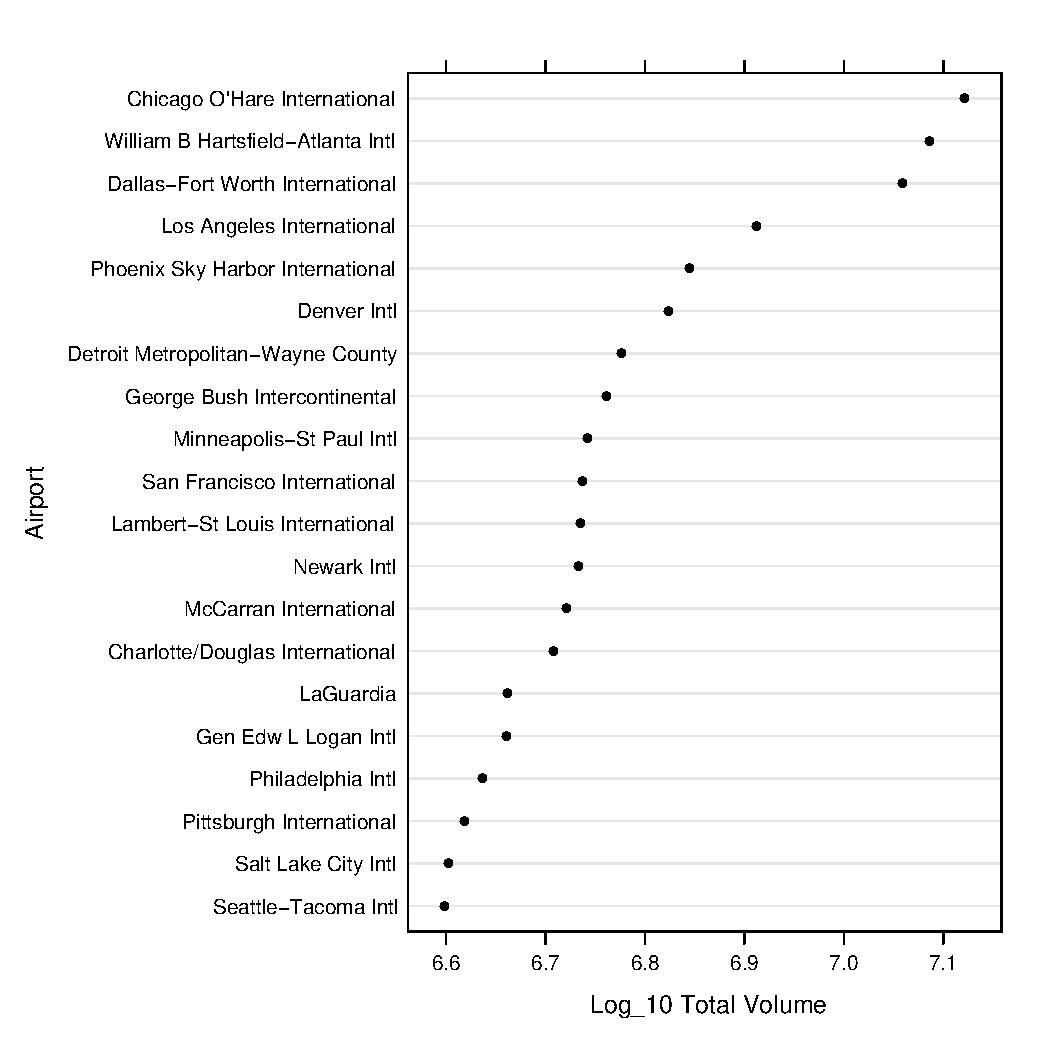
\includegraphics{volume.pdf}}
\caption{Top 20 airports by volume of all flights.}\end{figure}


\subsection{Carrier Popularity}
\label{airline:carrier-popularity}
Some carriers come and go, others demonstrate regular growth. In the following
display, the log base 10 volume (total flights) over years are displayed by
carrier. The carriers are ranked by their median volume (over the 10 year
span).

As mentioned before, RHIPE is mostly boilerplate. Notice the similarities
between this and previous examples (on a side note, to do this for 12GB of data
takes 1 minute and 32 seconds across 72 cores and all the examples, except the
download and conversion to R data frames, in the manual are less than 10 minutes)

\begin{Verbatim}[commandchars=\\\{\},numbers=left,firstnumber=1,stepnumber=1]
\PYG{c+c1}{\#\# To create summaries}
map \PYG{o}{\textless{}-} expression\PYG{p}{(}\PYG{p}{\PYGZob{}}
  a \PYG{o}{\textless{}-} do.call\PYG{p}{(}\PYG{l+s}{"}\PYG{l+s}{rbind"}\PYG{p}{,}map.values\PYG{p}{)}
  total \PYG{o}{\textless{}-} table\PYG{p}{(}years\PYG{o}{=}a\PYG{p}{[}\PYG{p}{,}\PYG{l+s}{'}\PYG{l+s}{year'}\PYG{p}{]}\PYG{p}{,}a\PYG{p}{[}\PYG{p}{,}\PYG{l+s}{'}\PYG{l+s}{carrier'}\PYG{p}{]}\PYG{p}{)}
  ac \PYG{o}{\textless{}-} rownames\PYG{p}{(}total\PYG{p}{)}
  ys \PYG{o}{\textless{}-} colnames\PYG{p}{(}total\PYG{p}{)}
  \PYG{k+kr}{for}\PYG{p}{(}yer in ac\PYG{p}{)}\PYG{p}{\PYGZob{}}
    \PYG{k+kr}{for}\PYG{p}{(}ca in ys\PYG{p}{)}\PYG{p}{\PYGZob{}}
      \PYG{k+kr}{if}\PYG{p}{(}total\PYG{p}{[}yer\PYG{p}{,}ca\PYG{p}{]}\PYG{o}{\textgreater{}}\PYG{l+m}{0}\PYG{p}{)} rhcollect\PYG{p}{(}c\PYG{p}{(}yer\PYG{p}{,}ca\PYG{p}{)}\PYG{p}{,} total\PYG{p}{[}yer\PYG{p}{,}ca\PYG{p}{]}\PYG{p}{)}
    \PYG{p}{\PYGZcb{}}
  \PYG{p}{\PYGZcb{}}
\PYG{p}{\PYGZcb{}}\PYG{p}{)}
reduce \PYG{o}{\textless{}-} expression\PYG{p}{(}
    pre\PYG{o}{=}\PYG{p}{\PYGZob{}}sums \PYG{o}{\textless{}-} \PYG{l+m}{0}\PYG{p}{\PYGZcb{}}\PYG{p}{,}
    reduce \PYG{o}{=} \PYG{p}{\PYGZob{}}sums \PYG{o}{\textless{}-} sums\PYG{o}{+}sum\PYG{p}{(}do.call\PYG{p}{(}\PYG{l+s}{"}\PYG{l+s}{rbind"}\PYG{p}{,}reduce.values\PYG{p}{)}\PYG{p}{)}\PYG{p}{\PYGZcb{}}\PYG{p}{,}
    post \PYG{o}{=} \PYG{p}{\PYGZob{}} rhcollect\PYG{p}{(}reduce.key\PYG{p}{,} sums\PYG{p}{)} \PYG{p}{\PYGZcb{}}
    \PYG{p}{)}

mapred \PYG{o}{\textless{}-} list\PYG{p}{(}\PYG{p}{)}
mapred\PYG{p}{\$}rhipe\PYGZus{}map\PYGZus{}buff\PYGZus{}size \PYG{o}{\textless{}-} \PYG{l+m}{5}
z \PYG{o}{\textless{}-} rhmr\PYG{p}{(}map\PYG{o}{=}map\PYG{p}{,}reduce\PYG{o}{=}reduce\PYG{p}{,}combiner\PYG{o}{=}\PYG{k+kc}{TRUE}\PYG{p}{,}inout\PYG{o}{=}c\PYG{p}{(}\PYG{l+s}{"}\PYG{l+s}{sequence"}\PYG{p}{,}\PYG{l+s}{"}\PYG{l+s}{sequence"}\PYG{p}{)}
          \PYG{p}{,}ifolder\PYG{o}{=}\PYG{l+s}{"}\PYG{l+s}{/airline/blocks/"}\PYG{p}{,}ofolder\PYG{o}{=}\PYG{l+s}{"}\PYG{l+s}{/airline/carrier.pop"}
          \PYG{p}{,}mapred\PYG{o}{=}mapred\PYG{p}{)}
z\PYG{o}{=}rhex\PYG{p}{(}z\PYG{p}{)}
\end{Verbatim}

This is the RHIPE code to create summaries. We need to extract the data from
Hadoop and create a display

\begin{Verbatim}[commandchars=\\\{\},numbers=left,firstnumber=1,stepnumber=1]
a \PYG{o}{\textless{}-} rhread\PYG{p}{(}\PYG{l+s}{"}\PYG{l+s}{/airline/carrier.pop"}\PYG{p}{)}
head\PYG{p}{(}a\PYG{p}{)}
\PYG{p}{[}\PYG{p}{[}\PYG{l+m}{1}\PYG{p}{]}\PYG{p}{]}
\PYG{p}{[}\PYG{p}{[}\PYG{l+m}{1}\PYG{p}{]}\PYG{p}{]}\PYG{p}{[}\PYG{p}{[}\PYG{l+m}{1}\PYG{p}{]}\PYG{p}{]}
\PYG{p}{[}\PYG{l+m}{1}\PYG{p}{]} \PYG{l+s}{"}\PYG{l+s}{90"} \PYG{l+s}{"}\PYG{l+s}{AA"}

\PYG{p}{[}\PYG{p}{[}\PYG{l+m}{1}\PYG{p}{]}\PYG{p}{]}\PYG{p}{[}\PYG{p}{[}\PYG{l+m}{2}\PYG{p}{]}\PYG{p}{]}
\PYG{p}{[}\PYG{l+m}{1}\PYG{p}{]} \PYG{l+m}{711825}


\PYG{p}{[}\PYG{p}{[}\PYG{l+m}{2}\PYG{p}{]}\PYG{p}{]}
\PYG{p}{[}\PYG{p}{[}\PYG{l+m}{2}\PYG{p}{]}\PYG{p}{]}\PYG{p}{[}\PYG{p}{[}\PYG{l+m}{1}\PYG{p}{]}\PYG{p}{]}
\PYG{p}{[}\PYG{l+m}{1}\PYG{p}{]} \PYG{l+s}{"}\PYG{l+s}{90"} \PYG{l+s}{"}\PYG{l+s}{AS"}

yr \PYG{o}{\textless{}-} as.numeric\PYG{p}{(}unlist\PYG{p}{(}lapply\PYG{p}{(}lapply\PYG{p}{(}a\PYG{p}{,}\PYG{l+s}{"}\PYG{l+s}{[["}\PYG{p}{,}\PYG{l+m}{1}\PYG{p}{)}\PYG{p}{,}\PYG{l+s}{"}\PYG{l+s}{[["}\PYG{p}{,}\PYG{l+m}{1}\PYG{p}{)}\PYG{p}{)}\PYG{p}{)}
carrier \PYG{o}{\textless{}-} unlist\PYG{p}{(}lapply\PYG{p}{(}lapply\PYG{p}{(}a\PYG{p}{,}\PYG{l+s}{"}\PYG{l+s}{[["}\PYG{p}{,}\PYG{l+m}{1}\PYG{p}{)}\PYG{p}{,}\PYG{l+s}{"}\PYG{l+s}{[["}\PYG{p}{,}\PYG{l+m}{2}\PYG{p}{)}\PYG{p}{)}
count \PYG{o}{\textless{}-} unlist\PYG{p}{(}lapply\PYG{p}{(}a\PYG{p}{,}\PYG{l+s}{"}\PYG{l+s}{[["}\PYG{p}{,}\PYG{l+m}{2}\PYG{p}{)}\PYG{p}{)}
results \PYG{o}{\textless{}-} data.frame\PYG{p}{(}yr\PYG{o}{=}yr\PYG{p}{,}carcode\PYG{o}{=}carrier\PYG{p}{,}count\PYG{o}{=}count\PYG{p}{,}stringsAsFactors\PYG{o}{=}\PYG{k+kc}{FALSE}\PYG{p}{)}
results \PYG{o}{\textless{}-} results\PYG{p}{[}order\PYG{p}{(}results\PYG{p}{\$}yr\PYG{p}{,}results\PYG{p}{\$}count\PYG{p}{,}decreasing\PYG{o}{=}\PYG{k+kc}{TRUE}\PYG{p}{)}\PYG{p}{,}\PYG{p}{]}
carrier \PYG{o}{\textless{}-} read.table\PYG{p}{(}\PYG{l+s}{"}\PYG{l+s}{\textasciitilde{}/tmp/carriers.csv"}\PYG{p}{,}sep\PYG{o}{=}\PYG{l+s}{"}\PYG{l+s}{,"}\PYG{p}{,}header\PYG{o}{=}\PYG{k+kc}{TRUE}\PYG{p}{,}
                      stringsAsFactors\PYG{o}{=}\PYG{k+kc}{FALSE}\PYG{p}{,}na.strings\PYG{o}{=}\PYG{l+s}{"}\PYG{l+s}{XYZB"}\PYG{p}{)}
results\PYG{p}{\$}carrier \PYG{o}{\textless{}-} sapply\PYG{p}{(}results\PYG{p}{\$}carcode\PYG{p}{,}\PYG{k+kr}{function}\PYG{p}{(}r\PYG{p}{)}\PYG{p}{\PYGZob{}}
  cd \PYG{o}{\textless{}-} carrier\PYG{p}{[}carrier\PYG{p}{\$}Code\PYG{o}{==}r\PYG{p}{,}\PYG{l+s}{'}\PYG{l+s}{Description'}\PYG{p}{]}
  \PYG{k+kr}{if}\PYG{p}{(}is.na\PYG{p}{(}cd\PYG{p}{)}\PYG{p}{)} r \PYG{k+kr}{else} cd
\PYG{p}{\PYGZcb{}}\PYG{p}{)}
results\PYG{p}{\$}yr \PYG{o}{\textless{}-} results\PYG{p}{\$}yr\PYG{o}{+}\PYG{l+m}{1900}
carr \PYG{o}{\textless{}-} reorder\PYG{p}{(}results\PYG{p}{\$}carrier\PYG{p}{,}results\PYG{p}{\$}count\PYG{p}{,} median\PYG{p}{)}
xyplot\PYG{p}{(}log\PYG{p}{(}count\PYG{p}{,}\PYG{l+m}{10}\PYG{p}{)}\textasciitilde{}yr\PYG{o}{\textbar{}}carr\PYG{p}{,} data\PYG{o}{=}results\PYG{p}{,}xlab\PYG{o}{=}\PYG{l+s}{"}\PYG{l+s}{Years"}\PYG{p}{,} ylab\PYG{o}{=}\PYG{l+s}{"}\PYG{l+s}{Log10 count"}\PYG{p}{,}col\PYG{o}{=}\PYG{l+s}{'}\PYG{l+s}{black'}
        \PYG{p}{,}scales\PYG{o}{=}list\PYG{p}{(}scale\PYG{o}{=}\PYG{l+s}{'}\PYG{l+s}{free'}\PYG{p}{,}tck\PYG{o}{=}\PYG{l+m}{0.5}\PYG{p}{,}cex\PYG{o}{=}\PYG{l+m}{0.7}\PYG{p}{)}\PYG{p}{,}layout\PYG{o}{=}c\PYG{p}{(}\PYG{l+m}{2}\PYG{p}{,}\PYG{l+m}{8}\PYG{p}{)}\PYG{p}{,}type\PYG{o}{=}\PYG{l+s}{'}\PYG{l+s}{l'}
       \PYG{p}{,}par.strip.text \PYG{o}{=} list\PYG{p}{(}lines \PYG{o}{=} \PYG{l+m}{0.8}\PYG{p}{,}cex\PYG{o}{=}\PYG{l+m}{0.7}\PYG{p}{)}\PYG{p}{,}cex\PYG{o}{=}\PYG{l+m}{0.5}\PYG{p}{,}
       panel\PYG{o}{=}\PYG{k+kr}{function}\PYG{p}{(}\PYG{l+m}{.}\PYG{l+m}{.}\PYG{l+m}{.}\PYG{p}{)}\PYG{p}{\PYGZob{}}
         panel.grid\PYG{p}{(}h\PYG{o}{=}\PYG{l+m}{-1}\PYG{p}{,}v\PYG{o}{=}\PYG{l+m}{-1}\PYG{p}{)}
         panel.xyplot\PYG{p}{(}\PYG{l+m}{.}\PYG{l+m}{.}\PYG{l+m}{.}\PYG{p}{)}
       \PYG{p}{\PYGZcb{}}\PYG{p}{)}
\end{Verbatim}

The graph is displayed above.


\subsection{Proportion of Flights Delayed}
\label{airline:proportion-of-flights-delayed}
Does this proportion increase with time? Consider the display with proportion of
flights delayed in a day across the years. Each year a panel. 22 panels. A
flight is delayed if the delay is greater than 15 minutes.

It is clear that proportion increases in the holidays (the ends of the
panels). The code for this comes after the figures.
\begin{figure}[htbp]
\centering

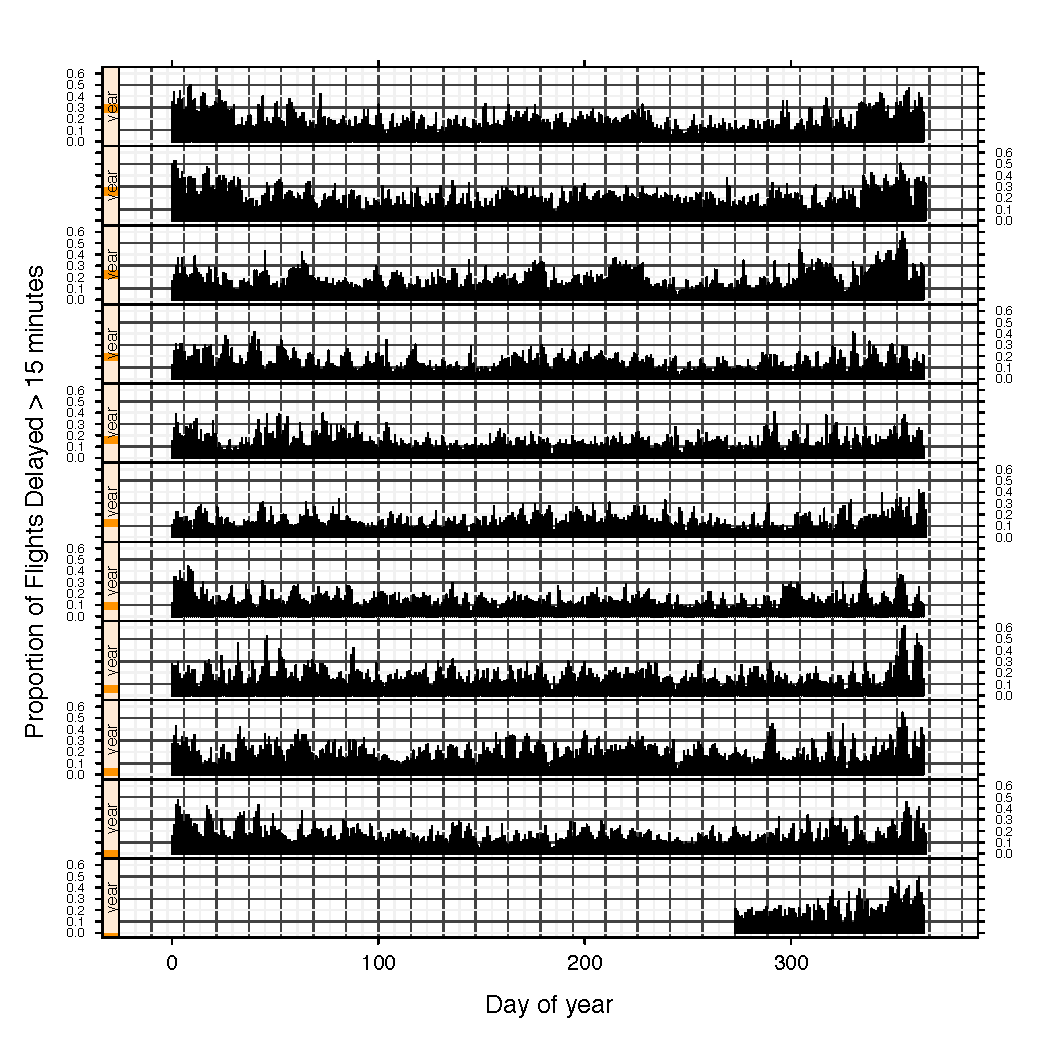
\includegraphics{propdelayed_1.pdf}
\caption{Proportion of flights delayed}\end{figure}
\begin{figure}[htbp]
\centering

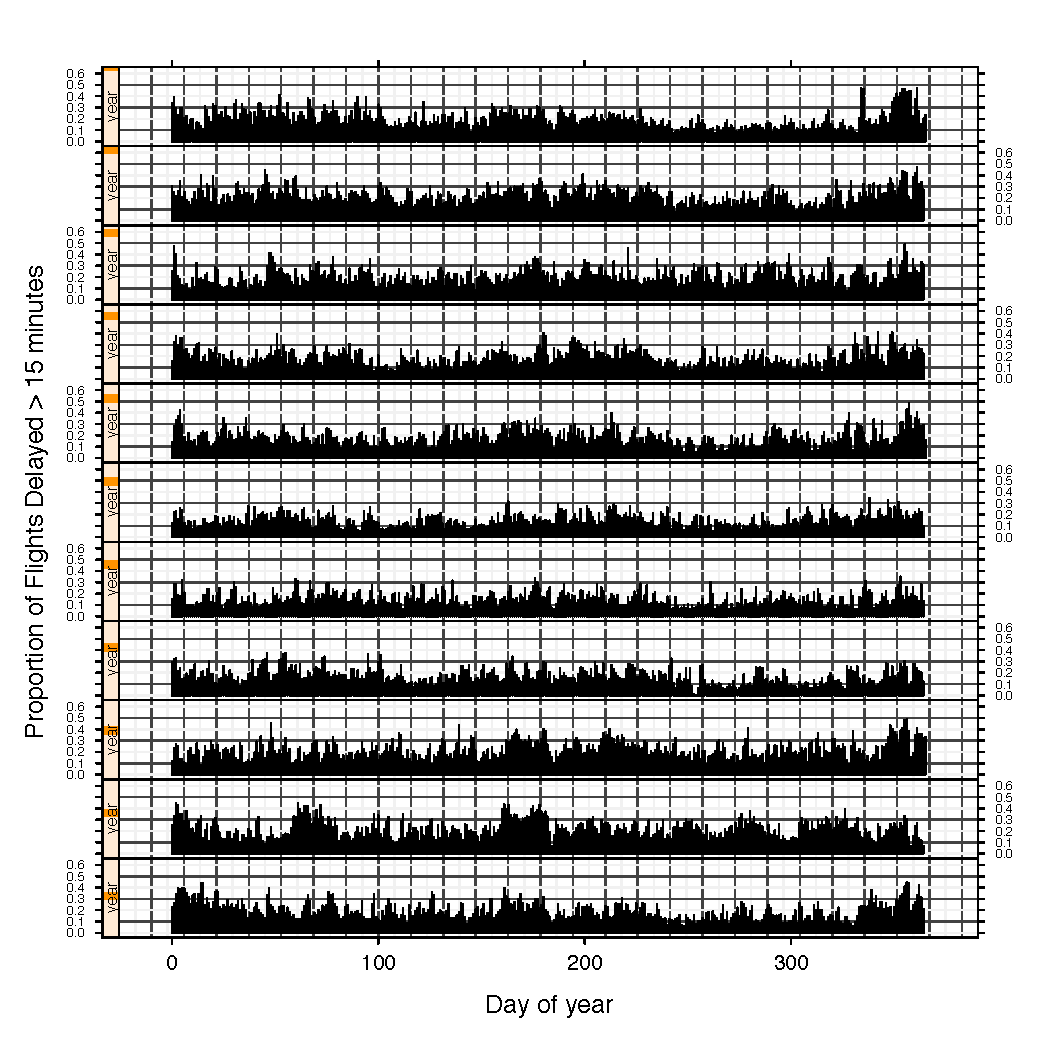
\includegraphics{propdelayed_2.pdf}
\caption{Proportion of flights delayed (cont'd)}\end{figure}

\begin{Verbatim}[commandchars=\\\{\},numbers=left,firstnumber=1,stepnumber=1]
map \PYG{o}{\textless{}-} expression\PYG{p}{(}\PYG{p}{\PYGZob{}}
  a \PYG{o}{\textless{}-} do.call\PYG{p}{(}\PYG{l+s}{"}\PYG{l+s}{rbind"}\PYG{p}{,}map.values\PYG{p}{)}
  a\PYG{p}{\$}delay.sec \PYG{o}{\textless{}-} as.vector\PYG{p}{(}a\PYG{p}{[}\PYG{p}{,}\PYG{l+s}{'}\PYG{l+s}{arrive'}\PYG{p}{]}\PYG{p}{)}\PYG{o}{-}as.vector\PYG{p}{(}a\PYG{p}{[}\PYG{p}{,}\PYG{l+s}{'}\PYG{l+s}{sarrive'}\PYG{p}{]}\PYG{p}{)}
  a \PYG{o}{\textless{}-} a\PYG{p}{[}!is.na\PYG{p}{(}a\PYG{p}{\$}delay.sec\PYG{p}{)}\PYG{p}{,}\PYG{p}{]}
  a\PYG{p}{\$}isdelayed \PYG{o}{\textless{}-} sapply\PYG{p}{(}a\PYG{p}{\$}delay.sec\PYG{p}{,}\PYG{k+kr}{function}\PYG{p}{(}r\PYG{p}{)} \PYG{k+kr}{if}\PYG{p}{(}r\PYG{o}{\textgreater{}=}\PYG{l+m}{900}\PYG{p}{)} \PYG{k+kc}{TRUE} \PYG{k+kr}{else} \PYG{k+kc}{FALSE}\PYG{p}{)}
  e \PYG{o}{\textless{}-} split\PYG{p}{(}a\PYG{p}{,}list\PYG{p}{(}a\PYG{p}{\$}year\PYG{p}{,}a\PYG{p}{\$}yday\PYG{p}{)}\PYG{p}{)}
  lapply\PYG{p}{(}e\PYG{p}{,}\PYG{k+kr}{function}\PYG{p}{(}r\PYG{p}{)}\PYG{p}{\PYGZob{}}
    n \PYG{o}{\textless{}-} nrow\PYG{p}{(}r\PYG{p}{)}\PYG{p}{;} numdelayed \PYG{o}{\textless{}-} sum\PYG{p}{(}r\PYG{p}{\$}isdelayed\PYG{p}{)}
    rhcollect\PYG{p}{(}as.vector\PYG{p}{(}unlist\PYG{p}{(}c\PYG{p}{(}r\PYG{p}{[}\PYG{l+m}{1}\PYG{p}{,}c\PYG{p}{(}\PYG{l+s}{"}\PYG{l+s}{year"}\PYG{p}{,}\PYG{l+s}{"}\PYG{l+s}{yday"}\PYG{p}{)}\PYG{p}{]}\PYG{p}{)}\PYG{p}{)}\PYG{p}{)}\PYG{p}{,} c\PYG{p}{(}n\PYG{p}{,} numdelayed\PYG{p}{)}\PYG{p}{)}
  \PYG{p}{\PYGZcb{}}\PYG{p}{)}
\PYG{p}{\PYGZcb{}}\PYG{p}{)}
reduce \PYG{o}{\textless{}-} expression\PYG{p}{(}
    pre\PYG{o}{=}\PYG{p}{\PYGZob{}}sums \PYG{o}{\textless{}-} c\PYG{p}{(}\PYG{l+m}{0}\PYG{p}{,}\PYG{l+m}{0}\PYG{p}{)}\PYG{p}{\PYGZcb{}}\PYG{p}{,}
    reduce \PYG{o}{=} \PYG{p}{\PYGZob{}}sums \PYG{o}{\textless{}-} sums\PYG{o}{+}apply\PYG{p}{(}do.call\PYG{p}{(}\PYG{l+s}{"}\PYG{l+s}{rbind"}\PYG{p}{,}reduce.values\PYG{p}{)}\PYG{p}{,}\PYG{l+m}{2}\PYG{p}{,}sum\PYG{p}{)}\PYG{p}{\PYGZcb{}}\PYG{p}{,}
    post \PYG{o}{=} \PYG{p}{\PYGZob{}} rhcollect\PYG{p}{(}reduce.key\PYG{p}{,} sums\PYG{p}{)} \PYG{p}{\PYGZcb{}}
    \PYG{p}{)}

mapred \PYG{o}{\textless{}-} list\PYG{p}{(}\PYG{p}{)}
mapred\PYG{p}{\$}rhipe\PYGZus{}map\PYGZus{}buff\PYGZus{}size \PYG{o}{\textless{}-} \PYG{l+m}{5}
z \PYG{o}{\textless{}-} rhmr\PYG{p}{(}map\PYG{o}{=}map\PYG{p}{,}reduce\PYG{o}{=}reduce\PYG{p}{,}combiner\PYG{o}{=}\PYG{k+kc}{TRUE}\PYG{p}{,}inout\PYG{o}{=}c\PYG{p}{(}\PYG{l+s}{"}\PYG{l+s}{sequence"}\PYG{p}{,}\PYG{l+s}{"}\PYG{l+s}{sequence"}\PYG{p}{)}
          \PYG{p}{,}ifolder\PYG{o}{=}\PYG{l+s}{"}\PYG{l+s}{/airline/blocks/"}\PYG{p}{,}ofolder\PYG{o}{=}\PYG{l+s}{"}\PYG{l+s}{/airline/delaybyyear"}
          \PYG{p}{,}mapred\PYG{o}{=}mapred\PYG{p}{)}
z\PYG{o}{=}rhex\PYG{p}{(}z\PYG{p}{)}

b \PYG{o}{\textless{}-} rhread\PYG{p}{(}\PYG{l+s}{"}\PYG{l+s}{/airline/delaybyyear"}\PYG{p}{)}
y1 \PYG{o}{\textless{}-} do.call\PYG{p}{(}\PYG{l+s}{"}\PYG{l+s}{rbind"}\PYG{p}{,}lapply\PYG{p}{(}b\PYG{p}{,}\PYG{l+s}{"}\PYG{l+s}{[["}\PYG{p}{,}\PYG{l+m}{1}\PYG{p}{)}\PYG{p}{)}
y2 \PYG{o}{\textless{}-} do.call\PYG{p}{(}\PYG{l+s}{"}\PYG{l+s}{rbind"}\PYG{p}{,}lapply\PYG{p}{(}b\PYG{p}{,}\PYG{l+s}{"}\PYG{l+s}{[["}\PYG{p}{,}\PYG{l+m}{2}\PYG{p}{)}\PYG{p}{)}
results \PYG{o}{\textless{}-} data.frame\PYG{p}{(}year\PYG{o}{=}\PYG{l+m}{1900}\PYG{o}{+}y1\PYG{p}{[}\PYG{p}{,}\PYG{l+m}{1}\PYG{p}{]}\PYG{p}{,}yday\PYG{o}{=}y1\PYG{p}{[}\PYG{p}{,}\PYG{l+m}{2}\PYG{p}{]}\PYG{p}{,}
                      nflight\PYG{o}{=}y2\PYG{p}{[}\PYG{p}{,}\PYG{l+m}{1}\PYG{p}{]}\PYG{p}{,}ndelay\PYG{o}{=}y2\PYG{p}{[}\PYG{p}{,}\PYG{l+m}{2}\PYG{p}{]}\PYG{p}{)}
results\PYG{p}{\$}prop \PYG{o}{\textless{}-} results\PYG{p}{\$}ndelay\PYG{o}{/}results\PYG{p}{\$}nflight
results \PYG{o}{\textless{}-} results\PYG{p}{[}order\PYG{p}{(}results\PYG{p}{\$}year\PYG{p}{,}results\PYG{p}{\$}yday\PYG{p}{)}\PYG{p}{,}\PYG{p}{]}
\end{Verbatim}

\hyperref[airline:stl-decomposition]{\emph{STL decomposition of proportion of flights delayed}} is
the STL decomposition of \emph{p} (the proportion of flights delayed). The \emph{seasonal}
panel clearly demonstrates the holiday effect of delays. They don't seem to be
increasing with time (see \emph{trend} panel).

\begin{Verbatim}[commandchars=\\\{\},numbers=left,firstnumber=1,stepnumber=1]
prop \PYG{o}{\textless{}-} results\PYG{p}{[}\PYG{p}{,}\PYG{l+s}{'}\PYG{l+s}{prop'}\PYG{p}{]}
prop \PYG{o}{\textless{}-} prop\PYG{p}{[}!is.na\PYG{p}{(}prop\PYG{p}{)}\PYG{p}{]}
tprop \PYG{o}{\textless{}-} ts\PYG{p}{(}log\PYG{p}{(}prop\PYG{o}{/}\PYG{p}{(}\PYG{l+m}{1}\PYG{o}{-}prop\PYG{p}{)}\PYG{p}{)}\PYG{p}{,}start\PYG{o}{=}c\PYG{p}{(}\PYG{l+m}{1987}\PYG{p}{,}\PYG{l+m}{273}\PYG{p}{)}\PYG{p}{,}frequency\PYG{o}{=}\PYG{l+m}{365}\PYG{p}{)}
pdf\PYG{p}{(}\PYG{l+s}{"}\PYG{l+s}{\textasciitilde{}/tmp/propdelayedxyplot.pdf"}\PYG{p}{)}
plot\PYG{p}{(}stl\PYG{p}{(}tprop\PYG{p}{,}s.window\PYG{o}{=}\PYG{l+s}{"}\PYG{l+s}{periodic"}\PYG{p}{)}\PYG{p}{)}
dev.off\PYG{p}{(}\PYG{p}{)}
\end{Verbatim}
\phantomsection\label{airline:stl-decomposition}\begin{figure}[htbp]
\centering

\scalebox{0.700000}{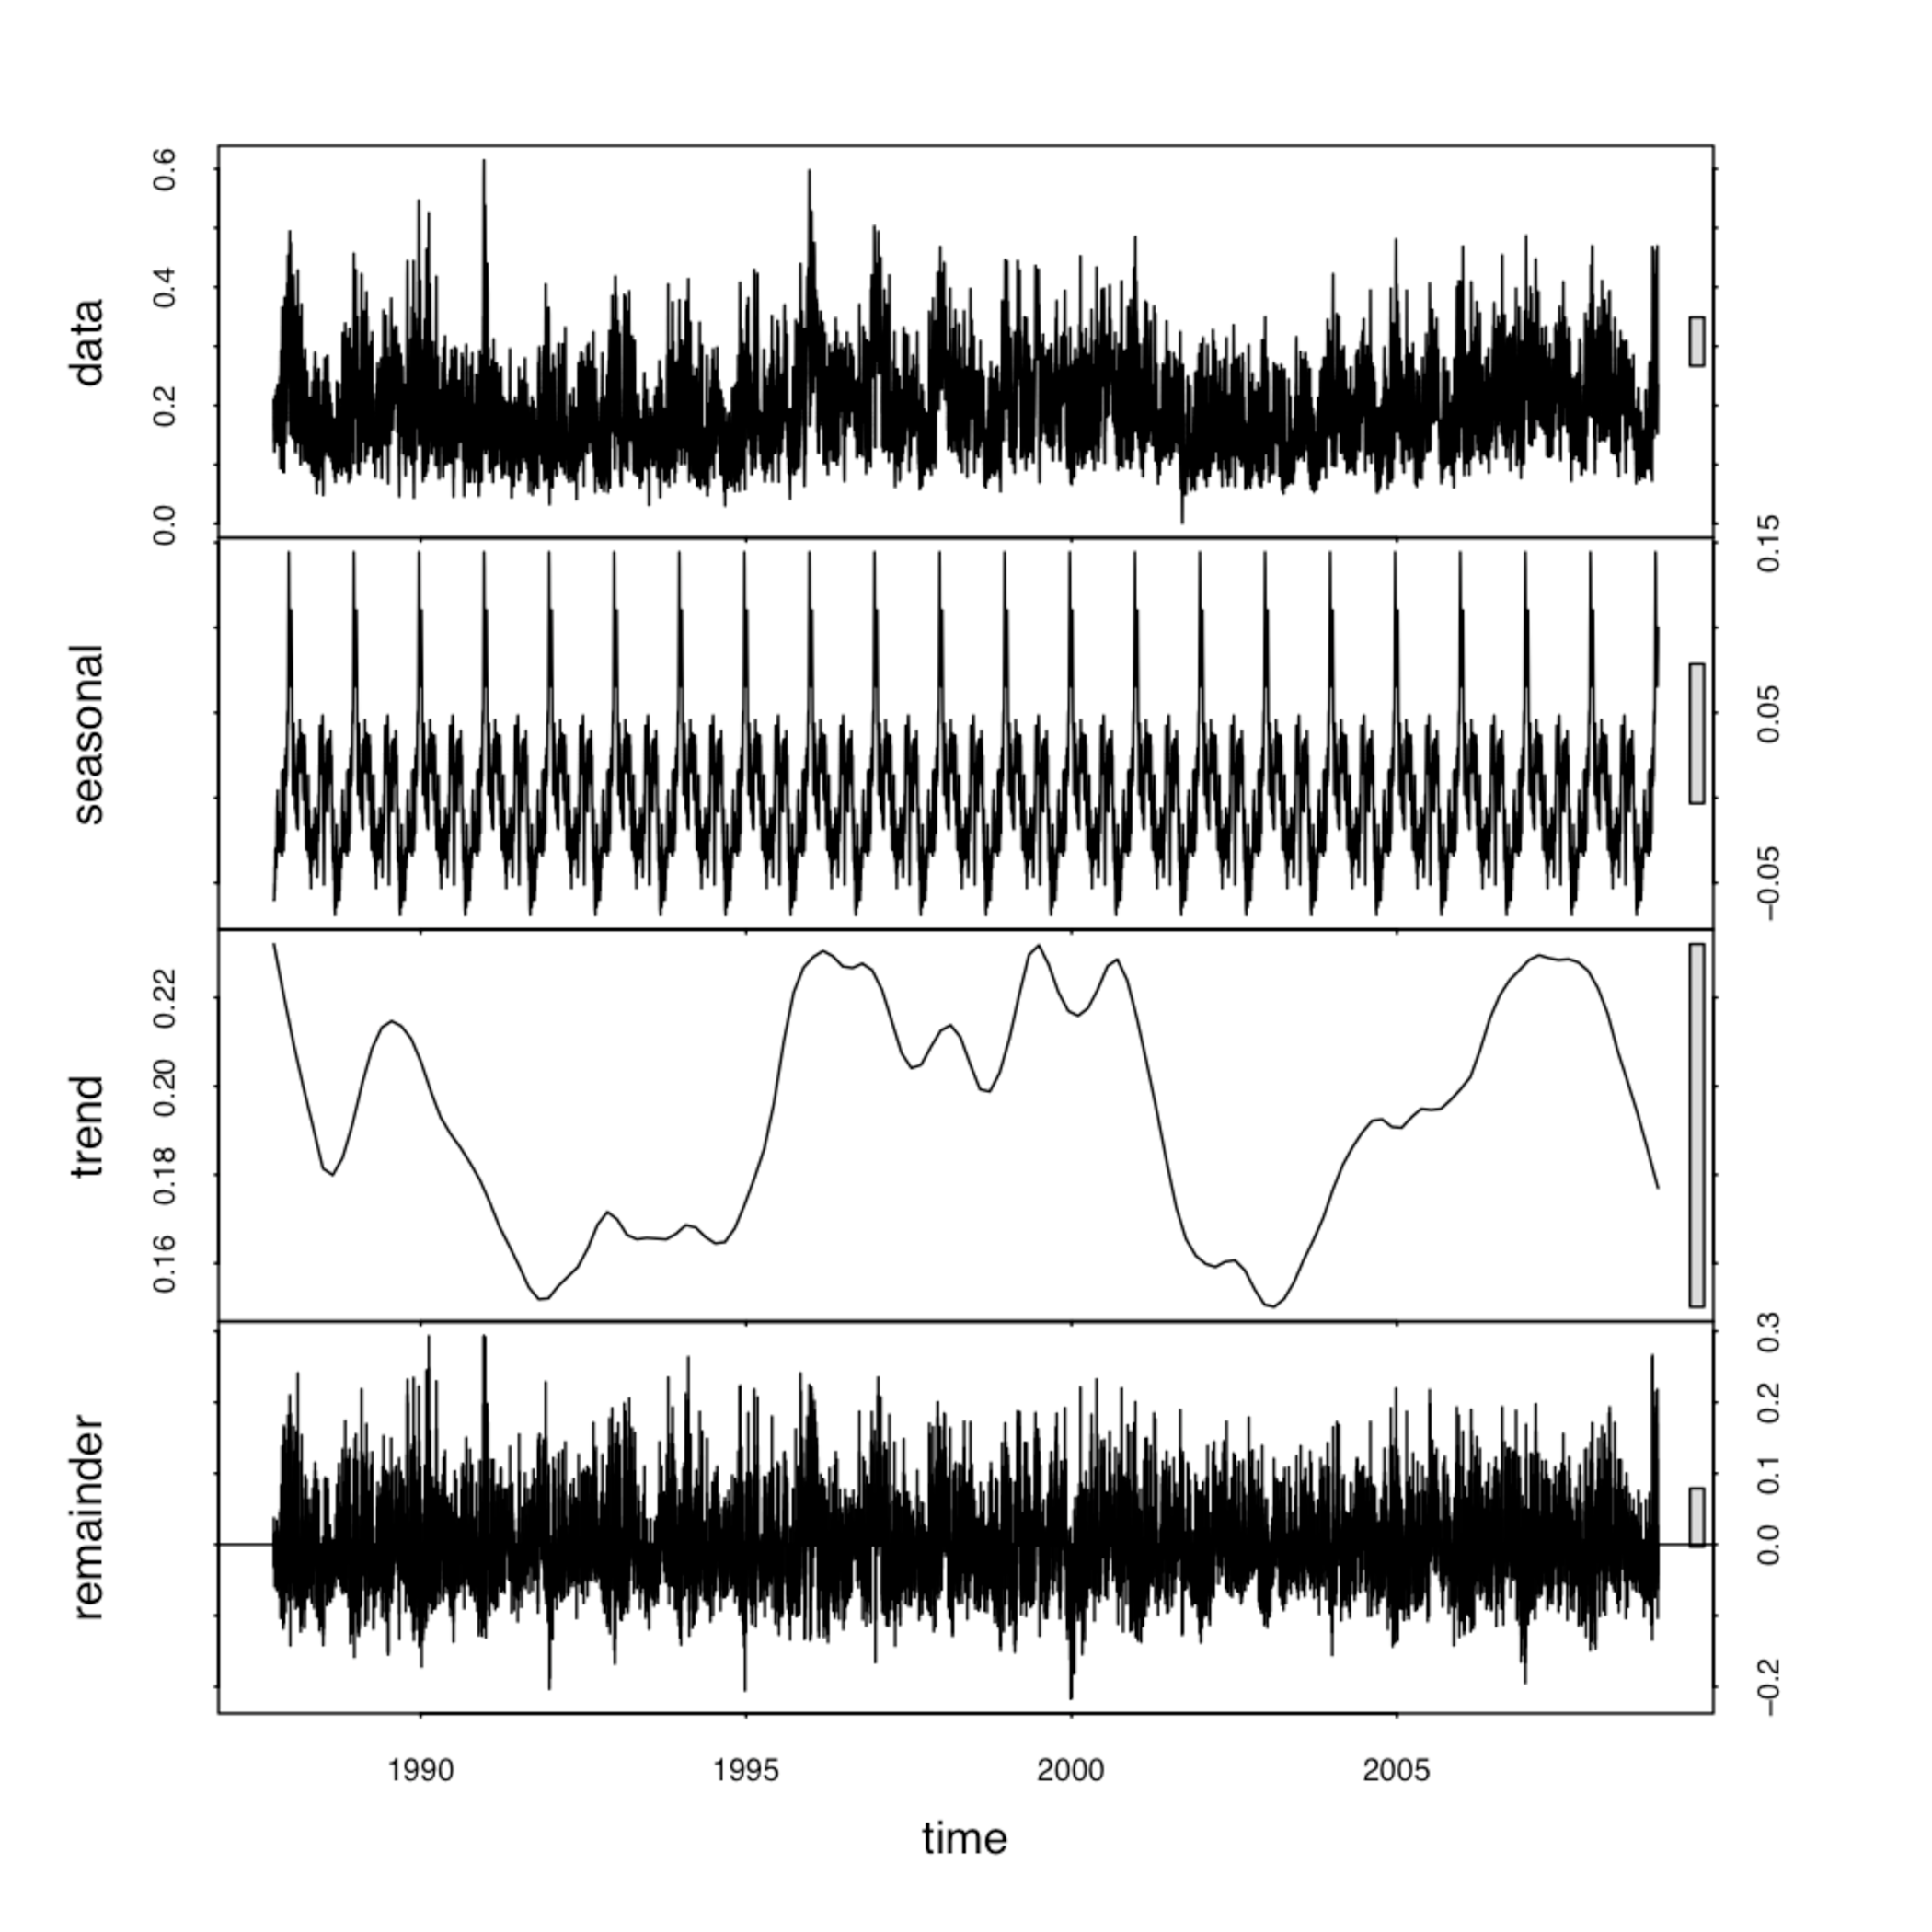
\includegraphics{propdelayedxyplot-fromtiff.pdf}}
\caption{STL decomposition of proportion of flights delayed}\end{figure}

There is similar seasonality for weekly behavior. The figure \hyperref[airline:delay-by-day-of-week]{\emph{Proportion of flights delayed by day of week.}} displays proportion of
flights delayed by day of week. The code for this identical to the previous one
except we split on \code{a\$wday} and the key is \code{r{[}1,c("wday"){]}}. It appears
Thursdays and Fridays can be quite trying.
\phantomsection\label{airline:delay-by-day-of-week}\begin{figure}[htbp]
\centering

\scalebox{0.700000}{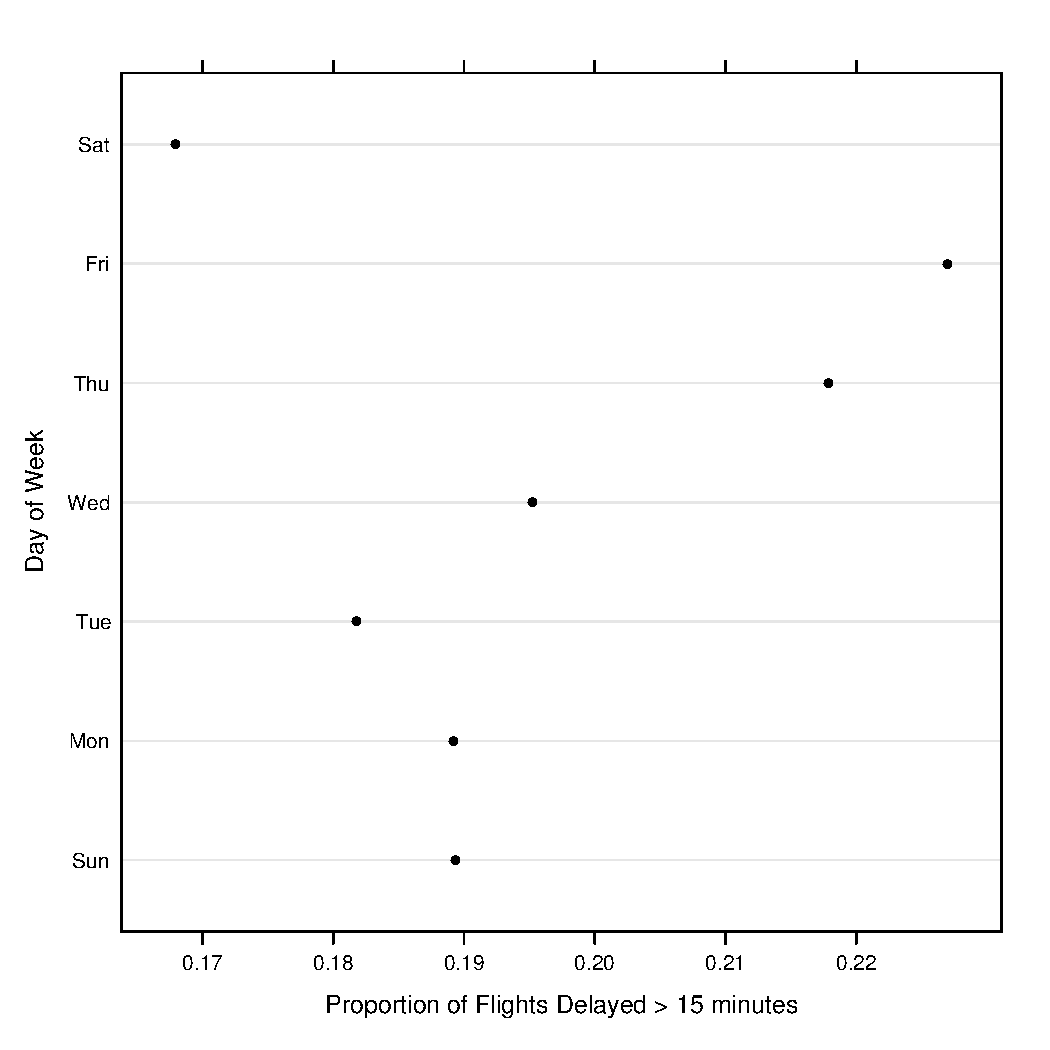
\includegraphics{propdelayeddow.pdf}}
\caption{Proportion of flights delayed by day of week.}\end{figure}

Does the delay proportion change with hour? It appears it does (see \hyperref[airline:delay-by-hour]{\emph{Proportion of flights delayed by hour of day}}). The hours are scheduled
departure times. \emph{Why are so many flights leaving in the wee hours (12-3) delayed?}
\phantomsection\label{airline:delay-by-hour}\begin{figure}[htbp]
\centering

\scalebox{0.700000}{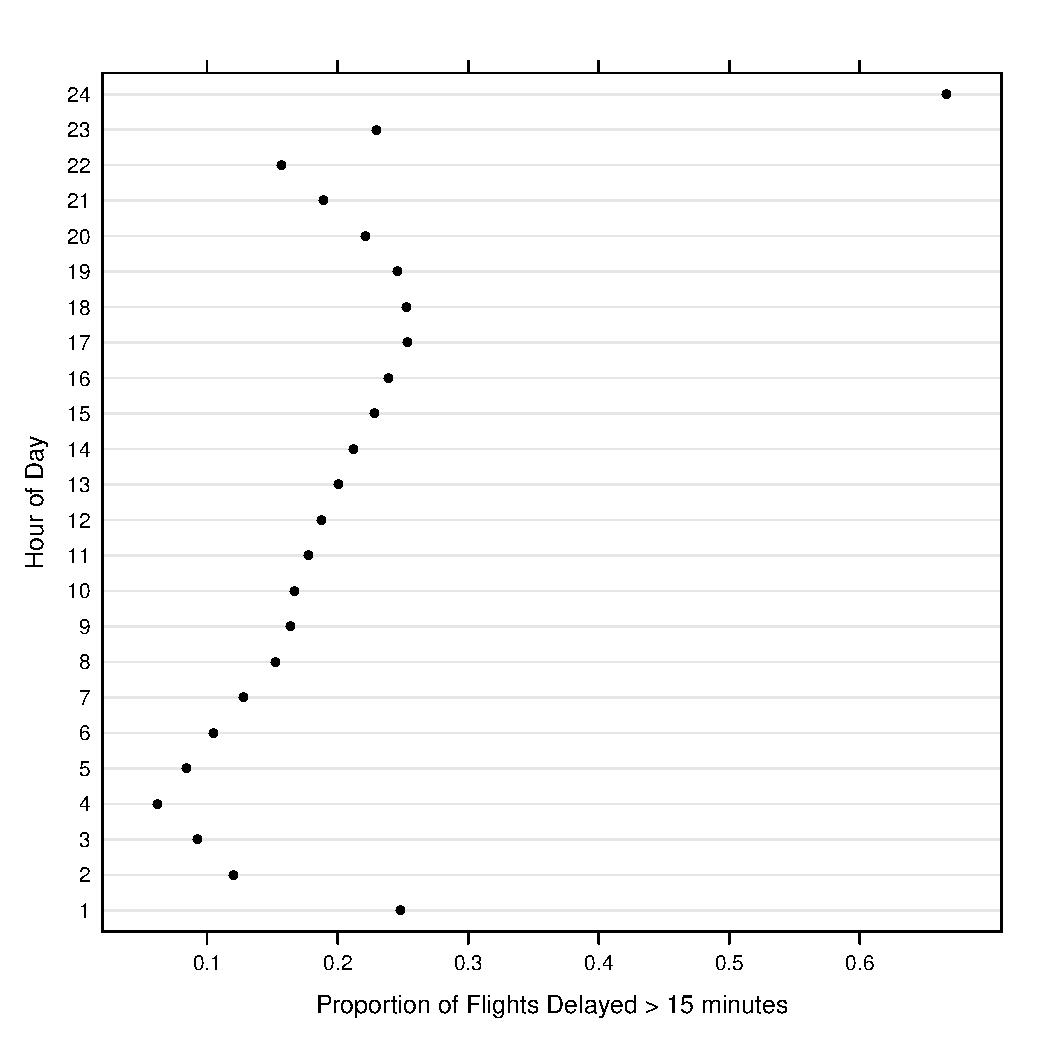
\includegraphics{propdelaybyhour.pdf}}
\caption{Proportion of flights delayed by hour of day}\end{figure}

The code to create \hyperref[airline:delay-by-hour]{\emph{Proportion of flights delayed by hour of day}} is

\begin{Verbatim}[commandchars=\\\{\},numbers=left,firstnumber=1,stepnumber=1]
map \PYG{o}{\textless{}-} expression\PYG{p}{(}\PYG{p}{\PYGZob{}}
  a \PYG{o}{\textless{}-} do.call\PYG{p}{(}\PYG{l+s}{"}\PYG{l+s}{rbind"}\PYG{p}{,}map.values\PYG{p}{)}
  a\PYG{p}{\$}delay.sec \PYG{o}{\textless{}-} as.vector\PYG{p}{(}a\PYG{p}{[}\PYG{p}{,}\PYG{l+s}{'}\PYG{l+s}{arrive'}\PYG{p}{]}\PYG{p}{)}\PYG{o}{-}as.vector\PYG{p}{(}a\PYG{p}{[}\PYG{p}{,}\PYG{l+s}{'}\PYG{l+s}{sarrive'}\PYG{p}{]}\PYG{p}{)}
  a \PYG{o}{\textless{}-} a\PYG{p}{[}!is.na\PYG{p}{(}a\PYG{p}{\$}delay.sec\PYG{p}{)}\PYG{p}{,}\PYG{p}{]}
  a\PYG{p}{\$}isdelayed \PYG{o}{\textless{}-} sapply\PYG{p}{(}a\PYG{p}{\$}delay.sec\PYG{p}{,}\PYG{k+kr}{function}\PYG{p}{(}r\PYG{p}{)} \PYG{k+kr}{if}\PYG{p}{(}r\PYG{o}{\textgreater{}=}\PYG{l+m}{900}\PYG{p}{)} \PYG{k+kc}{TRUE} \PYG{k+kr}{else} \PYG{k+kc}{FALSE}\PYG{p}{)}
  a\PYG{p}{\$}hrs \PYG{o}{\textless{}-} as.numeric\PYG{p}{(}format\PYG{p}{(}a\PYG{p}{[}\PYG{p}{,}\PYG{l+s}{'}\PYG{l+s}{sdepart'}\PYG{p}{]}\PYG{p}{,}\PYG{l+s}{"}\PYG{l+s}{\%H"}\PYG{p}{)}\PYG{p}{)}
  e \PYG{o}{\textless{}-} split\PYG{p}{(}a\PYG{p}{,}a\PYG{p}{\$}hrs\PYG{p}{)}
  lapply\PYG{p}{(}e\PYG{p}{,}\PYG{k+kr}{function}\PYG{p}{(}r\PYG{p}{)}\PYG{p}{\PYGZob{}}
    n \PYG{o}{\textless{}-} nrow\PYG{p}{(}r\PYG{p}{)}\PYG{p}{;} numdelayed \PYG{o}{\textless{}-} sum\PYG{p}{(}r\PYG{p}{\$}isdelayed\PYG{p}{)}
    rhcollect\PYG{p}{(}as.vector\PYG{p}{(}unlist\PYG{p}{(}c\PYG{p}{(}r\PYG{p}{[}\PYG{l+m}{1}\PYG{p}{,}c\PYG{p}{(}\PYG{l+s}{"}\PYG{l+s}{hrs"}\PYG{p}{)}\PYG{p}{]}\PYG{p}{)}\PYG{p}{)}\PYG{p}{)}\PYG{p}{,} c\PYG{p}{(}n\PYG{p}{,} numdelayed\PYG{p}{)}\PYG{p}{)}
  \PYG{p}{\PYGZcb{}}\PYG{p}{)}
\PYG{p}{\PYGZcb{}}\PYG{p}{)}
reduce \PYG{o}{\textless{}-} expression\PYG{p}{(}
    pre\PYG{o}{=}\PYG{p}{\PYGZob{}}sums \PYG{o}{\textless{}-} c\PYG{p}{(}\PYG{l+m}{0}\PYG{p}{,}\PYG{l+m}{0}\PYG{p}{)}\PYG{p}{\PYGZcb{}}\PYG{p}{,}
    reduce \PYG{o}{=} \PYG{p}{\PYGZob{}}sums \PYG{o}{\textless{}-} sums\PYG{o}{+}apply\PYG{p}{(}do.call\PYG{p}{(}\PYG{l+s}{"}\PYG{l+s}{rbind"}\PYG{p}{,}reduce.values\PYG{p}{)}\PYG{p}{,}\PYG{l+m}{2}\PYG{p}{,}sum\PYG{p}{)}\PYG{p}{\PYGZcb{}}\PYG{p}{,}
    post \PYG{o}{=} \PYG{p}{\PYGZob{}} rhcollect\PYG{p}{(}reduce.key\PYG{p}{,} sums\PYG{p}{)} \PYG{p}{\PYGZcb{}}
    \PYG{p}{)}


mapred \PYG{o}{\textless{}-} list\PYG{p}{(}\PYG{p}{)}
mapred\PYG{p}{\$}rhipe\PYGZus{}map\PYGZus{}buff\PYGZus{}size \PYG{o}{\textless{}-} \PYG{l+m}{5}
z \PYG{o}{\textless{}-} rhmr\PYG{p}{(}map\PYG{o}{=}map\PYG{p}{,}reduce\PYG{o}{=}reduce\PYG{p}{,}combiner\PYG{o}{=}\PYG{k+kc}{TRUE}\PYG{p}{,}inout\PYG{o}{=}c\PYG{p}{(}\PYG{l+s}{"}\PYG{l+s}{sequence"}\PYG{p}{,}\PYG{l+s}{"}\PYG{l+s}{sequence"}\PYG{p}{)}
          \PYG{p}{,}ifolder\PYG{o}{=}\PYG{l+s}{"}\PYG{l+s}{/airline/blocks/"}\PYG{p}{,}ofolder\PYG{o}{=}\PYG{l+s}{"}\PYG{l+s}{/airline/delaybyhours"}
          \PYG{p}{,}mapred\PYG{o}{=}mapred\PYG{p}{)}
z\PYG{o}{=}rhex\PYG{p}{(}z\PYG{p}{)}
\end{Verbatim}


\subsection{Distribution of Delays}
\label{airline:distribution-of-delays}
Summaries are not enough and for any sort of modeling we need to look at the
distribution of the data. So onto the quantiles of the delays. We will look at
delays greater than 15 minutes. To compute \emph{approximate} quantiles for the data,
we simply discretize the delay and compute a frequency count for the unique
values of delay. This is equivalent to binning the data. Given this frequency
table we can compute the quantiles.

The distribution of the delay in minutes does not change significantly over
months.
\index{quantiles}\phantomsection\label{airline:delay-quantiles-by-month}
\begin{Verbatim}[commandchars=\\\{\},numbers=left,firstnumber=1,stepnumber=1]
map \PYG{o}{\textless{}-} expression\PYG{p}{(}\PYG{p}{\PYGZob{}}
  a \PYG{o}{\textless{}-} do.call\PYG{p}{(}\PYG{l+s}{"}\PYG{l+s}{rbind"}\PYG{p}{,}map.values\PYG{p}{)}
  a\PYG{p}{\$}delay.sec \PYG{o}{\textless{}-} as.vector\PYG{p}{(}a\PYG{p}{[}\PYG{p}{,}\PYG{l+s}{'}\PYG{l+s}{arrive'}\PYG{p}{]}\PYG{p}{)}\PYG{o}{-}as.vector\PYG{p}{(}a\PYG{p}{[}\PYG{p}{,}\PYG{l+s}{'}\PYG{l+s}{sarrive'}\PYG{p}{]}\PYG{p}{)}
  a \PYG{o}{\textless{}-} a\PYG{p}{[}!is.na\PYG{p}{(}a\PYG{p}{\$}delay.sec\PYG{p}{)}\PYG{p}{,}\PYG{p}{]}
  a\PYG{p}{\$}isdelayed \PYG{o}{\textless{}-} sapply\PYG{p}{(}a\PYG{p}{\$}delay.sec\PYG{p}{,}\PYG{k+kr}{function}\PYG{p}{(}r\PYG{p}{)} \PYG{k+kr}{if}\PYG{p}{(}r\PYG{o}{\textgreater{}=}\PYG{l+m}{900}\PYG{p}{)} \PYG{k+kc}{TRUE} \PYG{k+kr}{else} \PYG{k+kc}{FALSE}\PYG{p}{)}
  a \PYG{o}{\textless{}-} a\PYG{p}{[}a\PYG{p}{\$}isdelayed\PYG{o}{==}\PYG{k+kc}{TRUE}\PYG{p}{,}\PYG{p}{]} \PYG{c+c1}{\#\# only look at delays greater than 15 minutes}
  apply\PYG{p}{(}a\PYG{p}{[}\PYG{p}{,}c\PYG{p}{(}\PYG{l+s}{'}\PYG{l+s}{month'}\PYG{p}{,}\PYG{l+s}{'}\PYG{l+s}{delay.sec'}\PYG{p}{)}\PYG{p}{]}\PYG{p}{,}\PYG{l+m}{1}\PYG{p}{,}\PYG{k+kr}{function}\PYG{p}{(}r\PYG{p}{)}\PYG{p}{\PYGZob{}}
        k \PYG{o}{\textless{}-} as.vector\PYG{p}{(}unlist\PYG{p}{(}r\PYG{p}{)}\PYG{p}{)}
        \PYG{k+kr}{if}\PYG{p}{(}!is.na\PYG{p}{(}k\PYG{p}{[}\PYG{l+m}{1}\PYG{p}{]}\PYG{p}{)}\PYG{p}{)} rhcollect\PYG{p}{(}k\PYG{p}{,}\PYG{l+m}{1}\PYG{p}{)} \PYG{c+c1}{\# ignore cases where month is missing}
      \PYG{p}{\PYGZcb{}}\PYG{p}{)}
\PYG{p}{\PYGZcb{}}\PYG{p}{)}
reduce \PYG{o}{\textless{}-} expression\PYG{p}{(}
    pre\PYG{o}{=}\PYG{p}{\PYGZob{}}sums \PYG{o}{\textless{}-} \PYG{l+m}{0}\PYG{p}{\PYGZcb{}} \PYG{p}{,}
    reduce \PYG{o}{=} \PYG{p}{\PYGZob{}}sums \PYG{o}{\textless{}-} sums\PYG{o}{+}sum\PYG{p}{(}unlist\PYG{p}{(}reduce.values\PYG{p}{)}\PYG{p}{)}\PYG{p}{\PYGZcb{}}\PYG{p}{,}
    post \PYG{o}{=} \PYG{p}{\PYGZob{}} rhcollect\PYG{p}{(}reduce.key\PYG{p}{,} sums\PYG{p}{)} \PYG{p}{\PYGZcb{}}
    \PYG{p}{)}
mapred \PYG{o}{\textless{}-} list\PYG{p}{(}\PYG{p}{)}
mapred\PYG{p}{\$}rhipe\PYGZus{}map\PYGZus{}buff\PYGZus{}size \PYG{o}{\textless{}-} \PYG{l+m}{5}
z \PYG{o}{\textless{}-} rhmr\PYG{p}{(}map\PYG{o}{=}map\PYG{p}{,}reduce\PYG{o}{=}reduce\PYG{p}{,}combiner\PYG{o}{=}\PYG{k+kc}{TRUE}\PYG{p}{,}inout\PYG{o}{=}c\PYG{p}{(}\PYG{l+s}{"}\PYG{l+s}{sequence"}\PYG{p}{,}\PYG{l+s}{"}\PYG{l+s}{sequence"}\PYG{p}{)}
          \PYG{p}{,}ifolder\PYG{o}{=}\PYG{l+s}{"}\PYG{l+s}{/airline/blocks/"}\PYG{p}{,}ofolder\PYG{o}{=}\PYG{l+s}{"}\PYG{l+s}{/airline/quantiledelay"}
          \PYG{p}{,}mapred\PYG{o}{=}mapred\PYG{p}{)}
z\PYG{o}{=}rhex\PYG{p}{(}z\PYG{p}{)}
b \PYG{o}{\textless{}-} rhread\PYG{p}{(}\PYG{l+s}{"}\PYG{l+s}{/airline/quantiledelay"}\PYG{p}{)}
y1 \PYG{o}{\textless{}-} do.call\PYG{p}{(}\PYG{l+s}{"}\PYG{l+s}{rbind"}\PYG{p}{,}lapply\PYG{p}{(}b\PYG{p}{,}\PYG{l+s}{"}\PYG{l+s}{[["}\PYG{p}{,}\PYG{l+m}{1}\PYG{p}{)}\PYG{p}{)}
count \PYG{o}{\textless{}-} do.call\PYG{p}{(}\PYG{l+s}{"}\PYG{l+s}{rbind"}\PYG{p}{,}lapply\PYG{p}{(}b\PYG{p}{,}\PYG{l+s}{"}\PYG{l+s}{[["}\PYG{p}{,}\PYG{l+m}{2}\PYG{p}{)}\PYG{p}{)}
results \PYG{o}{\textless{}-} data.frame\PYG{p}{(}month \PYG{o}{=} y1\PYG{p}{[}\PYG{p}{,}\PYG{l+m}{1}\PYG{p}{]}\PYG{p}{,} n\PYG{o}{=}y1\PYG{p}{[}\PYG{p}{,}\PYG{l+m}{2}\PYG{p}{]}\PYG{p}{,} count\PYG{o}{=}count\PYG{p}{)}
results \PYG{o}{\textless{}-} results\PYG{p}{[}order\PYG{p}{(}results\PYG{p}{\$}month\PYG{p}{,} results\PYG{p}{\$}n\PYG{p}{)}\PYG{p}{,}\PYG{p}{]}
results.2 \PYG{o}{\textless{}-} split\PYG{p}{(}results\PYG{p}{,} results\PYG{p}{\$}month\PYG{p}{)}

discrete.quantile\PYG{o}{\textless{}-}\PYG{k+kr}{function}\PYG{p}{(}x\PYG{p}{,}n\PYG{p}{,}prob\PYG{o}{=}seq\PYG{p}{(}\PYG{l+m}{0}\PYG{p}{,}\PYG{l+m}{1}\PYG{p}{,}\PYG{l+m}{0.25}\PYG{p}{)}\PYG{p}{,}type\PYG{o}{=}\PYG{l+m}{7}\PYG{p}{)}\PYG{p}{\PYGZob{}}
  sum.n\PYG{o}{\textless{}-}sum\PYG{p}{(}n\PYG{p}{)}
  cum.n\PYG{o}{\textless{}-}cumsum\PYG{p}{(}n\PYG{p}{)}
  np\PYG{o}{\textless{}-}\PYG{k+kr}{if}\PYG{p}{(}type\PYG{o}{==}\PYG{l+m}{7}\PYG{p}{)} \PYG{p}{(}sum.n\PYG{o}{-}\PYG{l+m}{1}\PYG{p}{)}\PYG{o}{*}prob\PYG{o}{+}\PYG{l+m}{1} \PYG{k+kr}{else} sum.n\PYG{o}{*}prob\PYG{o}{+}\PYG{l+m}{0.5}
  np.fl\PYG{o}{\textless{}-}floor\PYG{p}{(}np\PYG{p}{)}
  j1\PYG{o}{\textless{}-}pmax\PYG{p}{(}np.fl\PYG{p}{,}\PYG{l+m}{1}\PYG{p}{)}
  j2\PYG{o}{\textless{}-}pmin\PYG{p}{(}np.fl\PYG{o}{+}\PYG{l+m}{1}\PYG{p}{,}sum.n\PYG{p}{)}
  gamma\PYG{o}{\textless{}-}np\PYG{o}{-}np.fl
  id1\PYG{o}{\textless{}-}unlist\PYG{p}{(}lapply\PYG{p}{(}j1\PYG{p}{,}\PYG{k+kr}{function}\PYG{p}{(}r\PYG{p}{)} seq\PYGZus{}along\PYG{p}{(}cum.n\PYG{p}{)}\PYG{p}{[}r\PYG{o}{\textless{}=}cum.n\PYG{p}{]}\PYG{p}{[}\PYG{l+m}{1}\PYG{p}{]}\PYG{p}{)}\PYG{p}{)}
  id2\PYG{o}{\textless{}-}unlist\PYG{p}{(}lapply\PYG{p}{(}j2\PYG{p}{,}\PYG{k+kr}{function}\PYG{p}{(}r\PYG{p}{)} seq\PYGZus{}along\PYG{p}{(}cum.n\PYG{p}{)}\PYG{p}{[}r\PYG{o}{\textless{}=}cum.n\PYG{p}{]}\PYG{p}{[}\PYG{l+m}{1}\PYG{p}{]}\PYG{p}{)}\PYG{p}{)}
  x1\PYG{o}{\textless{}-}x\PYG{p}{[}id1\PYG{p}{]}
  x2\PYG{o}{\textless{}-}x\PYG{p}{[}id2\PYG{p}{]}
  qntl\PYG{o}{\textless{}-}\PYG{p}{(}\PYG{l+m}{1}\PYG{o}{-}gamma\PYG{p}{)}\PYG{o}{*}x1\PYG{o}{+}gamma\PYG{o}{*}x2
  qntl
\PYG{p}{\PYGZcb{}}

DEL \PYG{o}{\textless{}-} \PYG{l+m}{0.05}
results.3 \PYG{o}{\textless{}-} lapply\PYG{p}{(}seq\PYGZus{}along\PYG{p}{(}results.2\PYG{p}{)}\PYG{p}{,}\PYG{k+kr}{function}\PYG{p}{(}i\PYG{p}{)}\PYG{p}{\PYGZob{}}
  r \PYG{o}{\textless{}-} results.2\PYG{p}{[}\PYG{p}{[}i\PYG{p}{]}\PYG{p}{]}
  a \PYG{o}{\textless{}-} discrete.quantile\PYG{p}{(}r\PYG{p}{[}\PYG{p}{,}\PYG{l+m}{2}\PYG{p}{]}\PYG{p}{,}r\PYG{p}{[}\PYG{p}{,}\PYG{l+m}{3}\PYG{p}{]}\PYG{p}{,}prob\PYG{o}{=}seq\PYG{p}{(}\PYG{l+m}{0}\PYG{p}{,}\PYG{l+m}{1}\PYG{p}{,}DEL\PYG{p}{)}\PYG{p}{)}\PYG{o}{/}\PYG{l+m}{60}
  data.frame\PYG{p}{(}month\PYG{o}{=}as.numeric\PYG{p}{(}rep\PYG{p}{(}names\PYG{p}{(}results.2\PYG{p}{)}\PYG{p}{[}\PYG{p}{[}i\PYG{p}{]}\PYG{p}{]}\PYG{p}{,}length\PYG{p}{(}a\PYG{p}{)}\PYG{p}{)}\PYG{p}{)}\PYG{p}{,}prop\PYG{o}{=}seq\PYG{p}{(}\PYG{l+m}{0}\PYG{p}{,}\PYG{l+m}{1}\PYG{p}{,}DEL\PYG{p}{)}\PYG{p}{,}qt\PYG{o}{=}a\PYG{p}{)}
\PYG{p}{\PYGZcb{}}\PYG{p}{)}
results.3 \PYG{o}{\textless{}-} do.call\PYG{p}{(}\PYG{l+s}{"}\PYG{l+s}{rbind"}\PYG{p}{,}results.3\PYG{p}{)}
results.3\PYG{p}{\$}month \PYG{o}{\textless{}-} factor\PYG{p}{(}results.3\PYG{p}{\$}month\PYG{p}{,}
                          label\PYG{o}{=}c\PYG{p}{(}\PYG{l+s}{"}\PYG{l+s}{Jan"}\PYG{p}{,}\PYG{l+s}{"}\PYG{l+s}{Feb"}\PYG{p}{,}\PYG{l+s}{"}\PYG{l+s}{March"}\PYG{p}{,}\PYG{l+s}{"}\PYG{l+s}{Apr"}\PYG{p}{,}\PYG{l+s}{"}\PYG{l+s}{May"}\PYG{p}{,}\PYG{l+s}{"}\PYG{l+s}{June"}\PYG{p}{,}
                            \PYG{l+s}{"}\PYG{l+s}{July"}\PYG{p}{,}\PYG{l+s}{"}\PYG{l+s}{August"}\PYG{p}{,}\PYG{l+s}{"}\PYG{l+s}{September"}\PYG{p}{,}\PYG{l+s}{"}\PYG{l+s}{October"}\PYG{p}{,}\PYG{l+s}{"}\PYG{l+s}{November"}\PYG{p}{,}\PYG{l+s}{"}\PYG{l+s}{December"}\PYG{p}{)}\PYG{p}{)}
xyplot\PYG{p}{(}log\PYG{p}{(}qt\PYG{p}{,}\PYG{l+m}{2}\PYG{p}{)}\textasciitilde{}prop\PYG{o}{\textbar{}}month\PYG{p}{,} data\PYG{o}{=}results.3\PYG{p}{,}cex\PYG{o}{=}\PYG{l+m}{0.4}\PYG{p}{,}col\PYG{o}{=}\PYG{l+s}{'}\PYG{l+s}{black'}\PYG{p}{,}
       scales\PYG{o}{=}list\PYG{p}{(}x\PYG{o}{=}list\PYG{p}{(}tick.number\PYG{o}{=}\PYG{l+m}{10}\PYG{p}{)}\PYG{p}{,}y\PYG{o}{=}list\PYG{p}{(}tick.number\PYG{o}{=}\PYG{l+m}{10}\PYG{p}{)}\PYG{p}{)}\PYG{p}{,}
       layout\PYG{o}{=}c\PYG{p}{(}\PYG{l+m}{4}\PYG{p}{,}\PYG{l+m}{3}\PYG{p}{)}\PYG{p}{,}type\PYG{o}{=}\PYG{l+s}{'}\PYG{l+s}{l'}\PYG{p}{,}
       xlab\PYG{o}{=}\PYG{l+s}{"}\PYG{l+s}{Proportion"}\PYG{p}{,}ylab\PYG{o}{=}\PYG{l+s}{"}\PYG{l+s}{log\PYGZus{}2 delay (minutes)"}\PYG{p}{,}panel\PYG{o}{=}\PYG{k+kr}{function}\PYG{p}{(}x\PYG{p}{,}y\PYG{p}{,}\PYG{l+m}{.}\PYG{l+m}{.}\PYG{l+m}{.}\PYG{p}{)}\PYG{p}{\PYGZob{}}
         panel.grid\PYG{p}{(}h\PYG{o}{=}\PYG{l+m}{-1}\PYG{p}{,}v\PYG{o}{=}\PYG{l+m}{-1}\PYG{p}{)}\PYG{p}{;}panel.xyplot\PYG{p}{(}x\PYG{p}{,}y\PYG{p}{,}\PYG{l+m}{.}\PYG{l+m}{.}\PYG{l+m}{.}\PYG{p}{)}
       \PYG{p}{\PYGZcb{}}
\PYG{p}{)}
\end{Verbatim}
\begin{figure}[htbp]
\centering

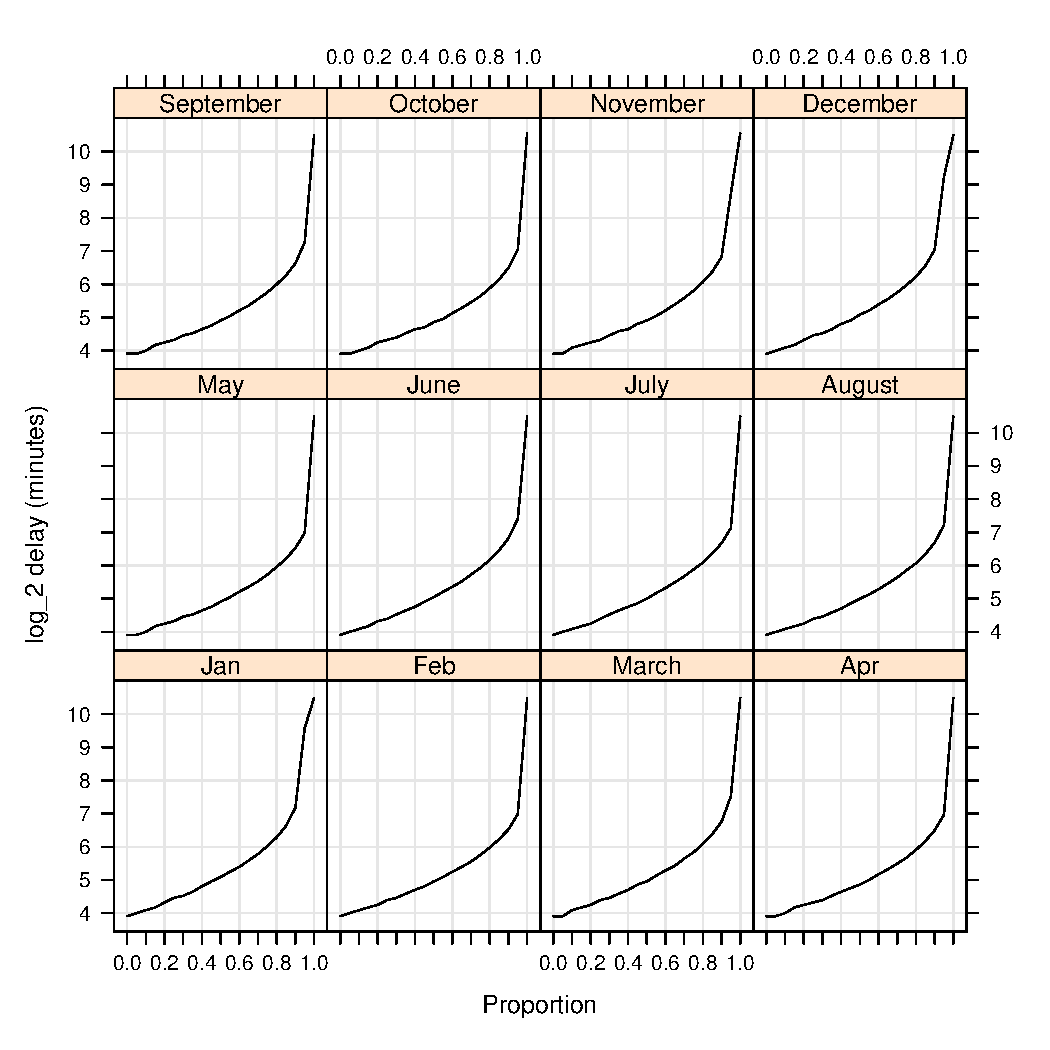
\includegraphics{quantiles_by_month.pdf}
\caption{Quantile of minute delay (for delay \textgreater{} 15 minutes) across months}\end{figure}

We can display the distribution by hour of day. The code is almost nearly the
same. Differences are in line 8, where the \code{hrs} is used as the conditioning.
But the results are more interesting. The delay amounts increase in the wee
hours (look at panel 23,24,1,2 and 3)

\begin{Verbatim}[commandchars=\\\{\},numbers=left,firstnumber=1,stepnumber=1]
map \PYG{o}{\textless{}-} expression\PYG{p}{(}\PYG{p}{\PYGZob{}}
  a \PYG{o}{\textless{}-} do.call\PYG{p}{(}\PYG{l+s}{"}\PYG{l+s}{rbind"}\PYG{p}{,}map.values\PYG{p}{)}
  a\PYG{p}{\$}delay.sec \PYG{o}{\textless{}-} as.vector\PYG{p}{(}a\PYG{p}{[}\PYG{p}{,}\PYG{l+s}{'}\PYG{l+s}{arrive'}\PYG{p}{]}\PYG{p}{)}\PYG{o}{-}as.vector\PYG{p}{(}a\PYG{p}{[}\PYG{p}{,}\PYG{l+s}{'}\PYG{l+s}{sarrive'}\PYG{p}{]}\PYG{p}{)}
  a \PYG{o}{\textless{}-} a\PYG{p}{[}!is.na\PYG{p}{(}a\PYG{p}{\$}delay.sec\PYG{p}{)}\PYG{p}{,}\PYG{p}{]}
  a\PYG{p}{\$}isdelayed \PYG{o}{\textless{}-} sapply\PYG{p}{(}a\PYG{p}{\$}delay.sec\PYG{p}{,}\PYG{k+kr}{function}\PYG{p}{(}r\PYG{p}{)} \PYG{k+kr}{if}\PYG{p}{(}r\PYG{o}{\textgreater{}=}\PYG{l+m}{900}\PYG{p}{)} \PYG{k+kc}{TRUE} \PYG{k+kr}{else} \PYG{k+kc}{FALSE}\PYG{p}{)}
  a \PYG{o}{\textless{}-} a\PYG{p}{[}a\PYG{p}{\$}isdelayed\PYG{o}{==}\PYG{k+kc}{TRUE}\PYG{p}{,}\PYG{p}{]} \PYG{c+c1}{\#\# only look at delays greater than 15 minutes}
  a\PYG{p}{\$}hrs \PYG{o}{\textless{}-} as.numeric\PYG{p}{(}format\PYG{p}{(}a\PYG{p}{[}\PYG{p}{,}\PYG{l+s}{'}\PYG{l+s}{sdepart'}\PYG{p}{]}\PYG{p}{,}\PYG{l+s}{"}\PYG{l+s}{\%H"}\PYG{p}{)}\PYG{p}{)}
  apply\PYG{p}{(}a\PYG{p}{[}\PYG{p}{,}c\PYG{p}{(}\PYG{l+s}{'}\PYG{l+s}{hrs'}\PYG{p}{,}\PYG{l+s}{'}\PYG{l+s}{delay.sec'}\PYG{p}{)}\PYG{p}{]}\PYG{p}{,}\PYG{l+m}{1}\PYG{p}{,}\PYG{k+kr}{function}\PYG{p}{(}r\PYG{p}{)}\PYG{p}{\PYGZob{}}
        k \PYG{o}{\textless{}-} as.vector\PYG{p}{(}unlist\PYG{p}{(}r\PYG{p}{)}\PYG{p}{)}
        \PYG{k+kr}{if}\PYG{p}{(}!is.na\PYG{p}{(}k\PYG{p}{[}\PYG{l+m}{1}\PYG{p}{]}\PYG{p}{)}\PYG{p}{)} rhcollect\PYG{p}{(}k\PYG{p}{,}\PYG{l+m}{1}\PYG{p}{)}
      \PYG{p}{\PYGZcb{}}\PYG{p}{)}
\PYG{p}{\PYGZcb{}}\PYG{p}{)}
reduce \PYG{o}{\textless{}-} expression\PYG{p}{(}
    pre\PYG{o}{=}\PYG{p}{\PYGZob{}}sums \PYG{o}{\textless{}-} \PYG{l+m}{0}\PYG{p}{\PYGZcb{}} \PYG{p}{,}
    reduce \PYG{o}{=} \PYG{p}{\PYGZob{}}sums \PYG{o}{\textless{}-} sums\PYG{o}{+}sum\PYG{p}{(}unlist\PYG{p}{(}reduce.values\PYG{p}{)}\PYG{p}{)}\PYG{p}{\PYGZcb{}}\PYG{p}{,}
    post \PYG{o}{=} \PYG{p}{\PYGZob{}} rhcollect\PYG{p}{(}reduce.key\PYG{p}{,} sums\PYG{p}{)} \PYG{p}{\PYGZcb{}}
    \PYG{p}{)}

mapred \PYG{o}{\textless{}-} list\PYG{p}{(}\PYG{p}{)}
mapred\PYG{p}{\$}rhipe\PYGZus{}map\PYGZus{}buff\PYGZus{}size \PYG{o}{\textless{}-} \PYG{l+m}{5}
z \PYG{o}{\textless{}-} rhmr\PYG{p}{(}map\PYG{o}{=}map\PYG{p}{,}reduce\PYG{o}{=}reduce\PYG{p}{,}combiner\PYG{o}{=}\PYG{k+kc}{TRUE}\PYG{p}{,}inout\PYG{o}{=}c\PYG{p}{(}\PYG{l+s}{"}\PYG{l+s}{sequence"}\PYG{p}{,}\PYG{l+s}{"}\PYG{l+s}{sequence"}\PYG{p}{)}
          \PYG{p}{,}ifolder\PYG{o}{=}\PYG{l+s}{"}\PYG{l+s}{/airline/blocks/"}\PYG{p}{,}ofolder\PYG{o}{=}\PYG{l+s}{"}\PYG{l+s}{/airline/quantiledelaybyhour"}
          \PYG{p}{,}mapred\PYG{o}{=}mapred\PYG{p}{)}
z\PYG{o}{=}rhex\PYG{p}{(}z\PYG{p}{)}
\end{Verbatim}
\begin{figure}[htbp]
\centering

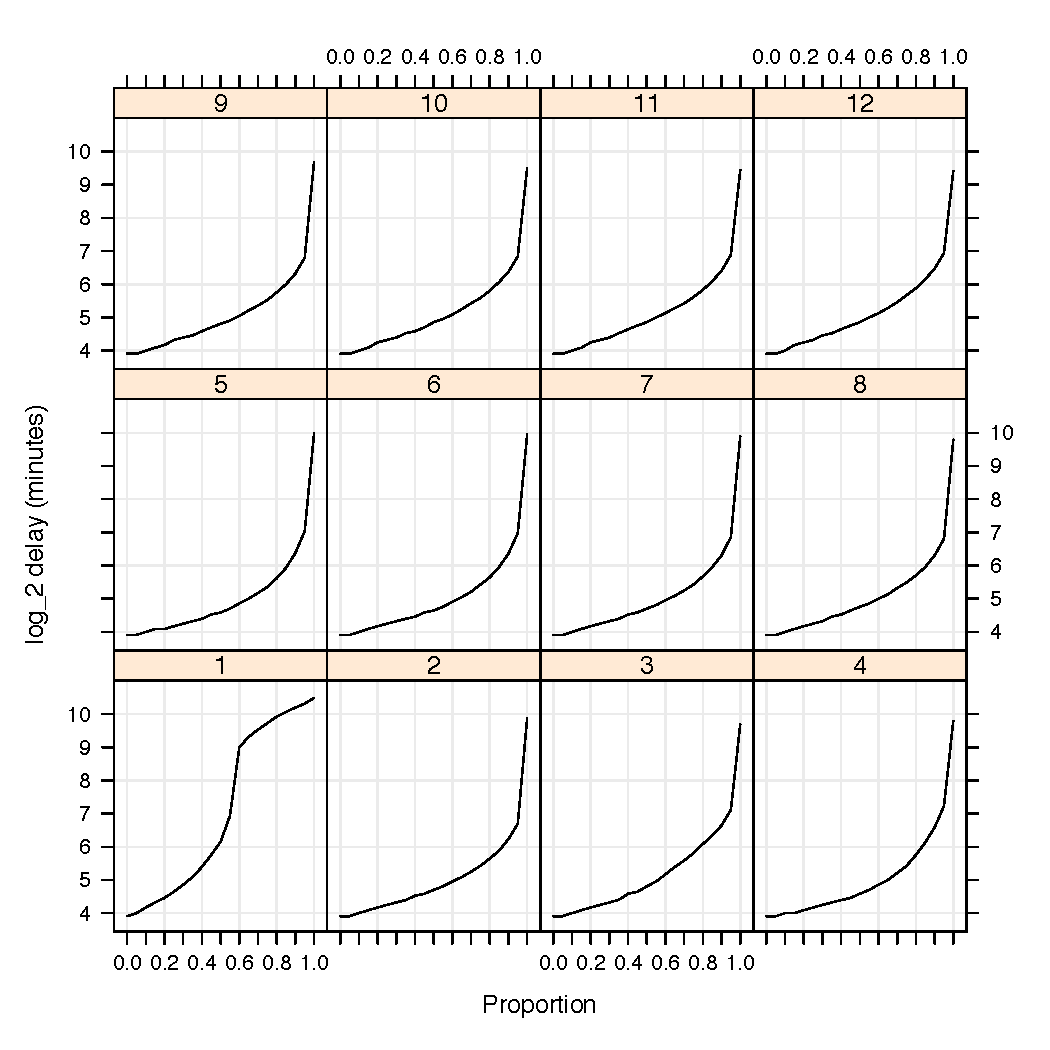
\includegraphics{quantiles_by_hr_1.pdf}
\caption{Quantile of minute delay (for delay \textgreater{} 15 minutes) by hour of day}\end{figure}
\begin{figure}[htbp]
\centering

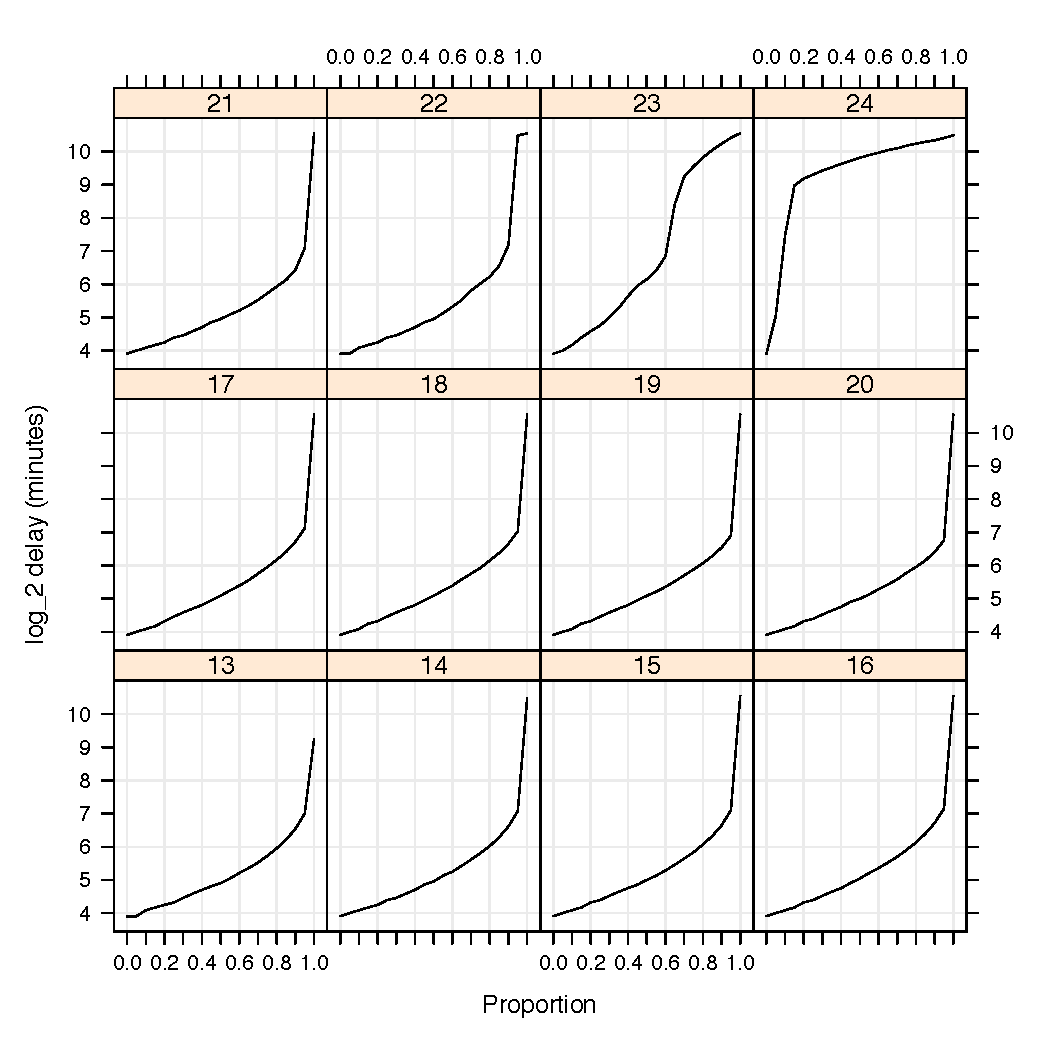
\includegraphics{quantiles_by_hr_2.pdf}
\caption{Quantile of minute delay (for delay \textgreater{} 15 minutes) by hour of day (cont'd)}\end{figure}

The distribution of delay times by airports. This could be analyzed for several
airports, but we take the top 3 in terms of volumes. In this display, the
quantiles of log\_2 of the delay times (in minutes) for inbound and outbound for
4 different airports is plotted. The airports are in order of median delay time.
Of note, the median delay time for Chicago (ORD) and San Francisco (SFO) is greater flying in than out
(approximately an hour). For both Chicago and Dallas Fort Worth (DFW), the 75th
percentile of inbound delays is greater than that for outbound. \hyperref[airline:quantilebyairport]{\emph{Quantile of minute delay for inbound and outbound for 4 different
airports. Dotted red lines are 25\%,50\% and 75\% uniform proportions.}} displays these differences.

\begin{Verbatim}[commandchars=\\\{\},numbers=left,firstnumber=1,stepnumber=1]
 map \PYG{o}{\textless{}-} expression\PYG{p}{(}\PYG{p}{\PYGZob{}}
   cc \PYG{o}{\textless{}-} c\PYG{p}{(}\PYG{l+s}{"}\PYG{l+s}{ORD"}\PYG{p}{,}\PYG{l+s}{"}\PYG{l+s}{SEA"}\PYG{p}{,}\PYG{l+s}{"}\PYG{l+s}{DFW"}\PYG{p}{,}\PYG{l+s}{"}\PYG{l+s}{SFO"}\PYG{p}{)}
   a \PYG{o}{\textless{}-} do.call\PYG{p}{(}\PYG{l+s}{"}\PYG{l+s}{rbind"}\PYG{p}{,}map.values\PYG{p}{)}
   a \PYG{o}{\textless{}-} a\PYG{p}{[}a\PYG{p}{\$}origin \PYG{o}{\%in\%} cc\PYG{o}{\textbar{}} a\PYG{p}{\$}dest \PYG{o}{\%in\%} cc\PYG{p}{,}\PYG{p}{]}
   \PYG{k+kr}{if}\PYG{p}{(}nrow\PYG{p}{(}a\PYG{p}{)}\PYG{o}{\textgreater{}}\PYG{l+m}{0}\PYG{p}{)}\PYG{p}{\PYGZob{}}
     a\PYG{p}{\$}delay.sec \PYG{o}{\textless{}-} as.vector\PYG{p}{(}a\PYG{p}{[}\PYG{p}{,}\PYG{l+s}{'}\PYG{l+s}{arrive'}\PYG{p}{]}\PYG{p}{)}\PYG{o}{-}as.vector\PYG{p}{(}a\PYG{p}{[}\PYG{p}{,}\PYG{l+s}{'}\PYG{l+s}{sarrive'}\PYG{p}{]}\PYG{p}{)}
     a \PYG{o}{\textless{}-} a\PYG{p}{[}!is.na\PYG{p}{(}a\PYG{p}{\$}delay.sec\PYG{p}{)}\PYG{p}{,}\PYG{p}{]}
     a\PYG{p}{\$}isdelayed \PYG{o}{\textless{}-} sapply\PYG{p}{(}a\PYG{p}{\$}delay.sec\PYG{p}{,}\PYG{k+kr}{function}\PYG{p}{(}r\PYG{p}{)} \PYG{k+kr}{if}\PYG{p}{(}r\PYG{o}{\textgreater{}=}\PYG{l+m}{900}\PYG{p}{)} \PYG{k+kc}{TRUE} \PYG{k+kr}{else} \PYG{k+kc}{FALSE}\PYG{p}{)}
     a \PYG{o}{\textless{}-} a\PYG{p}{[}a\PYG{p}{\$}isdelayed\PYG{o}{==}\PYG{k+kc}{TRUE}\PYG{p}{,}\PYG{p}{]}
     \PYG{k+kr}{for}\PYG{p}{(}i in \PYG{l+m}{1}:nrow\PYG{p}{(}a\PYG{p}{)}\PYG{p}{)}\PYG{p}{\PYGZob{}}
       dl \PYG{o}{\textless{}-} a\PYG{p}{[}i\PYG{p}{,}\PYG{l+s}{'}\PYG{l+s}{delay.sec'}\PYG{p}{]}
       \PYG{k+kr}{if}\PYG{p}{(}a\PYG{p}{[}i\PYG{p}{,}\PYG{l+s}{'}\PYG{l+s}{origin'}\PYG{p}{]} \PYG{o}{\%in\%} cc\PYG{p}{)} rhcollect\PYG{p}{(}data.frame\PYG{p}{(}dir\PYG{o}{=}\PYG{l+s}{"}\PYG{l+s}{outbound"}\PYG{p}{,}ap\PYG{o}{=}a\PYG{p}{[}i\PYG{p}{,}\PYG{l+s}{"}\PYG{l+s}{origin"}\PYG{p}{]}
                                                      \PYG{p}{,}delay\PYG{o}{=}dl\PYG{p}{,}stringsAsFactors\PYG{o}{=}\PYG{k+kc}{FALSE}\PYG{p}{)}\PYG{p}{,}\PYG{l+m}{1}\PYG{p}{)}
       \PYG{k+kr}{if}\PYG{p}{(}a\PYG{p}{[}i\PYG{p}{,}\PYG{l+s}{'}\PYG{l+s}{dest'}\PYG{p}{]} \PYG{o}{\%in\%} cc\PYG{p}{)} rhcollect\PYG{p}{(}data.frame\PYG{p}{(}dir\PYG{o}{=}\PYG{l+s}{"}\PYG{l+s}{inbound"}\PYG{p}{,}ap\PYG{o}{=}a\PYG{p}{[}i\PYG{p}{,}\PYG{l+s}{"}\PYG{l+s}{dest"}\PYG{p}{]}
                                               \PYG{p}{,}delay\PYG{o}{=}dl\PYG{p}{,}stringsAsFactors\PYG{o}{=}\PYG{k+kc}{FALSE}\PYG{p}{)}\PYG{p}{,}\PYG{l+m}{1}\PYG{p}{)}
     \PYG{p}{\PYGZcb{}}
   \PYG{p}{\PYGZcb{}}
 \PYG{p}{\PYGZcb{}}\PYG{p}{)}
reduce \PYG{o}{\textless{}-} expression\PYG{p}{(}
     pre\PYG{o}{=}\PYG{p}{\PYGZob{}}sums \PYG{o}{\textless{}-} \PYG{l+m}{0}\PYG{p}{\PYGZcb{}} \PYG{p}{,}
     reduce \PYG{o}{=} \PYG{p}{\PYGZob{}}sums \PYG{o}{\textless{}-} sums\PYG{o}{+}sum\PYG{p}{(}unlist\PYG{p}{(}reduce.values\PYG{p}{)}\PYG{p}{)}\PYG{p}{\PYGZcb{}}\PYG{p}{,}
     post \PYG{o}{=} \PYG{p}{\PYGZob{}} rhcollect\PYG{p}{(}reduce.key\PYG{p}{,} sums\PYG{p}{)} \PYG{p}{\PYGZcb{}}
     \PYG{p}{)}
 mapred \PYG{o}{\textless{}-} list\PYG{p}{(}\PYG{p}{)}
 mapred\PYG{p}{\$}rhipe\PYGZus{}map\PYGZus{}buff\PYGZus{}size \PYG{o}{\textless{}-} \PYG{l+m}{5}
 z \PYG{o}{\textless{}-} rhmr\PYG{p}{(}map\PYG{o}{=}map\PYG{p}{,}reduce\PYG{o}{=}reduce\PYG{p}{,}combiner\PYG{o}{=}\PYG{k+kc}{TRUE}\PYG{p}{,}inout\PYG{o}{=}c\PYG{p}{(}\PYG{l+s}{"}\PYG{l+s}{sequence"}\PYG{p}{,}\PYG{l+s}{"}\PYG{l+s}{sequence"}\PYG{p}{)}
           \PYG{p}{,}ifolder\PYG{o}{=}\PYG{l+s}{"}\PYG{l+s}{/airline/blocks/"}\PYG{p}{,}ofolder\PYG{o}{=}\PYG{l+s}{"}\PYG{l+s}{/airline/inoutboundelay"}
           \PYG{p}{,}mapred\PYG{o}{=}mapred\PYG{p}{)}
 z\PYG{o}{=}rhex\PYG{p}{(}z\PYG{p}{)}
\end{Verbatim}
\phantomsection\label{airline:quantilebyairport}\begin{figure}[htbp]
\centering

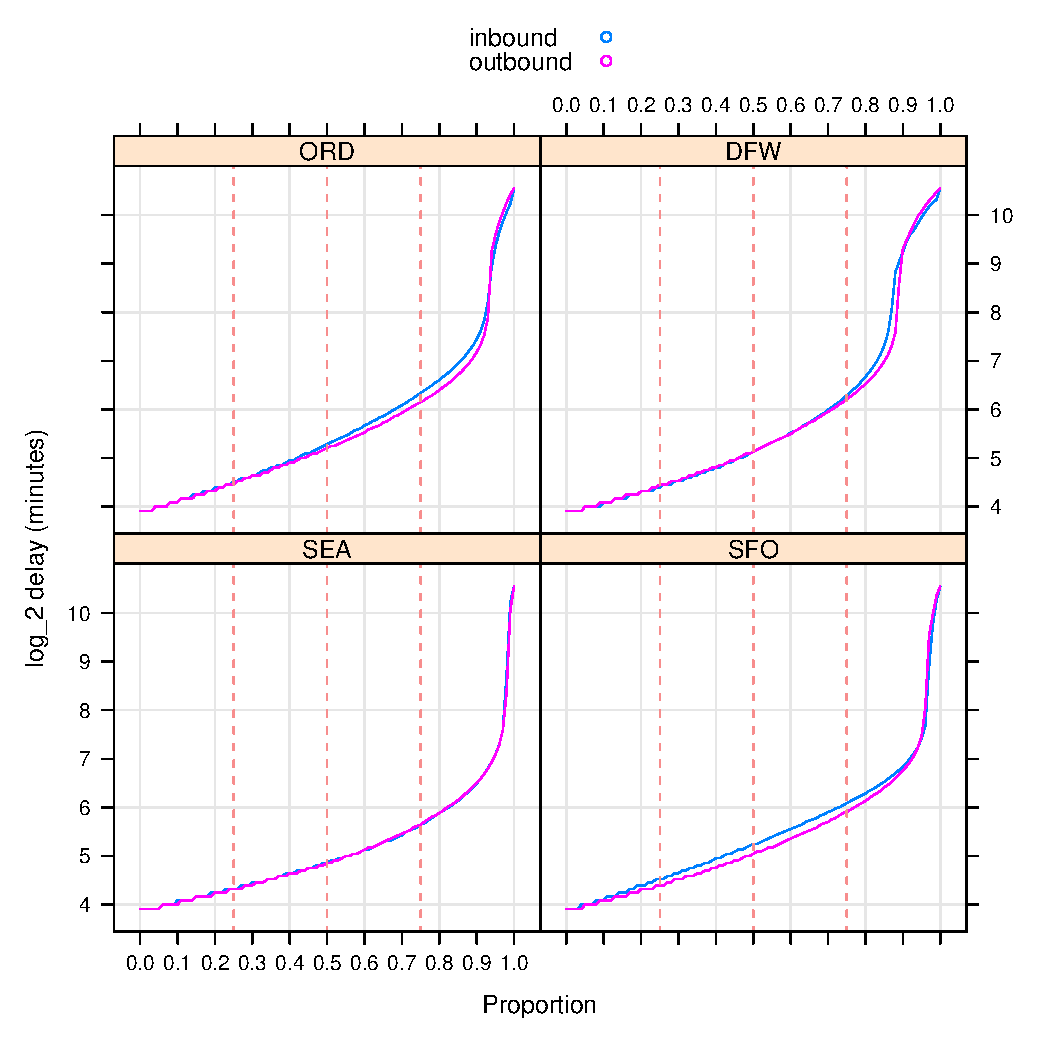
\includegraphics{quantiles_by_airport.pdf}
\caption{Quantile of minute delay for inbound and outbound for 4 different
airports. Dotted red lines are 25\%,50\% and 75\% uniform proportions.}\end{figure}


\subsection{Carrier Delays}
\label{airline:carrier-delays}
Is there a difference in carrier delays? We display the time series of
proportion of delayed flights by carrier, ranked by carrier.

\begin{Verbatim}[commandchars=\\\{\},numbers=left,firstnumber=1,stepnumber=1]
\PYG{c+c1}{\#\# For proportions and volumes}
map \PYG{o}{\textless{}-} expression\PYG{p}{(}\PYG{p}{\PYGZob{}}
  a \PYG{o}{\textless{}-} do.call\PYG{p}{(}\PYG{l+s}{"}\PYG{l+s}{rbind"}\PYG{p}{,}map.values\PYG{p}{)}
  a\PYG{p}{\$}delay.sec \PYG{o}{\textless{}-} as.vector\PYG{p}{(}a\PYG{p}{[}\PYG{p}{,}\PYG{l+s}{'}\PYG{l+s}{arrive'}\PYG{p}{]}\PYG{p}{)}\PYG{o}{-}as.vector\PYG{p}{(}a\PYG{p}{[}\PYG{p}{,}\PYG{l+s}{'}\PYG{l+s}{sarrive'}\PYG{p}{]}\PYG{p}{)}
  a \PYG{o}{\textless{}-} a\PYG{p}{[}!is.na\PYG{p}{(}a\PYG{p}{\$}delay.sec\PYG{p}{)}\PYG{p}{,}\PYG{p}{]}
  a\PYG{p}{\$}isdelayed \PYG{o}{\textless{}-} sapply\PYG{p}{(}a\PYG{p}{\$}delay.sec\PYG{p}{,}\PYG{k+kr}{function}\PYG{p}{(}r\PYG{p}{)} \PYG{k+kr}{if}\PYG{p}{(}r\PYG{o}{\textgreater{}=}\PYG{l+m}{900}\PYG{p}{)} \PYG{k+kc}{TRUE} \PYG{k+kr}{else} \PYG{k+kc}{FALSE}\PYG{p}{)}
  a\PYG{p}{\$}hrs \PYG{o}{\textless{}-} as.numeric\PYG{p}{(}format\PYG{p}{(}a\PYG{p}{[}\PYG{p}{,}\PYG{l+s}{'}\PYG{l+s}{sdepart'}\PYG{p}{]}\PYG{p}{,}\PYG{l+s}{"}\PYG{l+s}{\%H"}\PYG{p}{)}\PYG{p}{)}
  e \PYG{o}{\textless{}-} split\PYG{p}{(}a\PYG{p}{,}a\PYG{p}{\$}hrs\PYG{p}{)}
  lapply\PYG{p}{(}e\PYG{p}{,}\PYG{k+kr}{function}\PYG{p}{(}r\PYG{p}{)}\PYG{p}{\PYGZob{}}
    n \PYG{o}{\textless{}-} nrow\PYG{p}{(}r\PYG{p}{)}\PYG{p}{;} numdelayed \PYG{o}{\textless{}-} sum\PYG{p}{(}r\PYG{p}{\$}isdelayed\PYG{p}{)}
    rhcollect\PYG{p}{(}as.vector\PYG{p}{(}unlist\PYG{p}{(}c\PYG{p}{(}r\PYG{p}{[}\PYG{l+m}{1}\PYG{p}{,}c\PYG{p}{(}\PYG{l+s}{"}\PYG{l+s}{carrier"}\PYG{p}{)}\PYG{p}{]}\PYG{p}{)}\PYG{p}{)}\PYG{p}{)}\PYG{p}{,} c\PYG{p}{(}n\PYG{p}{,} numdelayed\PYG{p}{)}\PYG{p}{)}
  \PYG{p}{\PYGZcb{}}\PYG{p}{)}
\PYG{p}{\PYGZcb{}}\PYG{p}{)}
reduce \PYG{o}{\textless{}-} expression\PYG{p}{(}
    pre\PYG{o}{=}\PYG{p}{\PYGZob{}}sums \PYG{o}{\textless{}-} c\PYG{p}{(}\PYG{l+m}{0}\PYG{p}{,}\PYG{l+m}{0}\PYG{p}{)}\PYG{p}{\PYGZcb{}}\PYG{p}{,}
    reduce \PYG{o}{=} \PYG{p}{\PYGZob{}}sums \PYG{o}{\textless{}-} sums\PYG{o}{+}apply\PYG{p}{(}do.call\PYG{p}{(}\PYG{l+s}{"}\PYG{l+s}{rbind"}\PYG{p}{,}reduce.values\PYG{p}{)}\PYG{p}{,}\PYG{l+m}{2}\PYG{p}{,}sum\PYG{p}{)}\PYG{p}{\PYGZcb{}}\PYG{p}{,}
    post \PYG{o}{=} \PYG{p}{\PYGZob{}} rhcollect\PYG{p}{(}reduce.key\PYG{p}{,} sums\PYG{p}{)} \PYG{p}{\PYGZcb{}}
    \PYG{p}{)}
\end{Verbatim}
\begin{figure}[htbp]
\centering

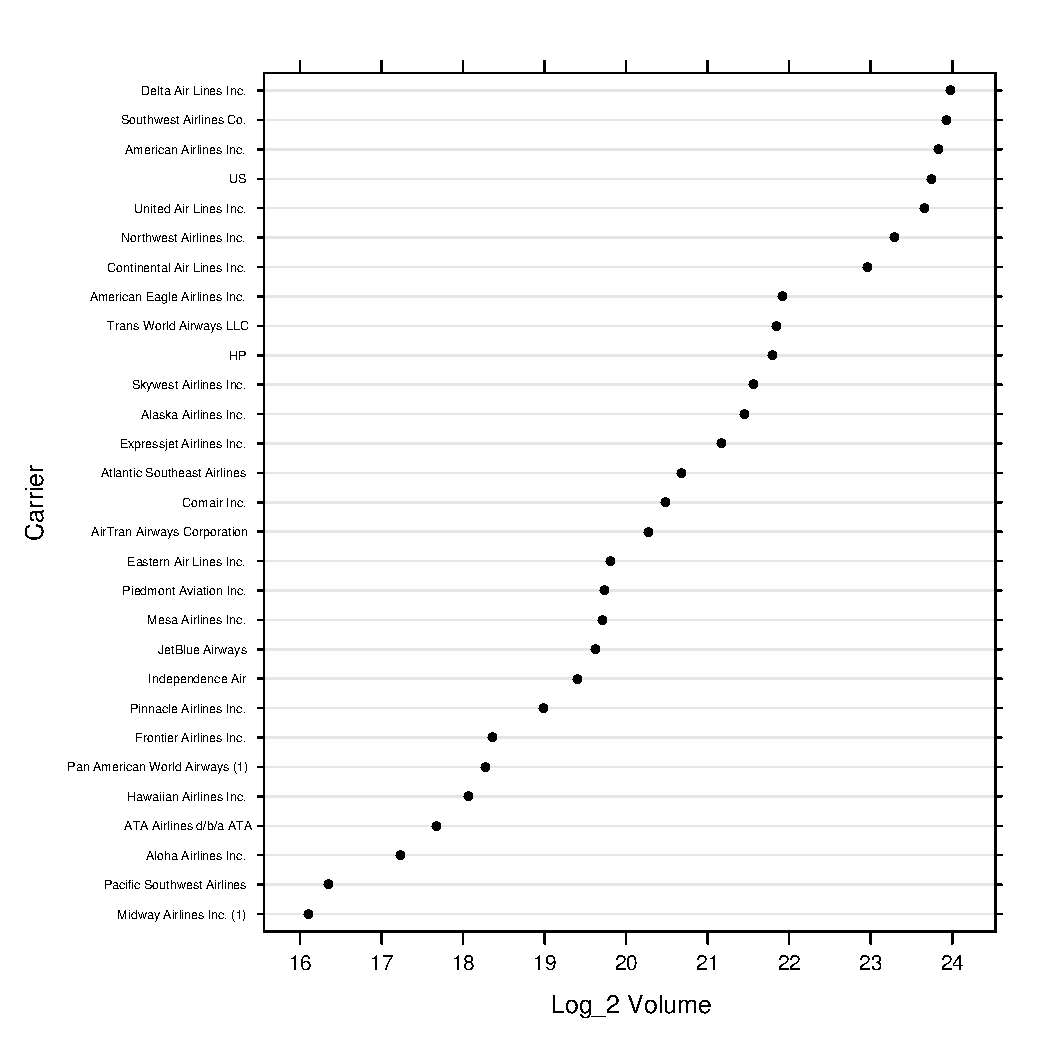
\includegraphics{carrvol.pdf}
\caption{Log base 2 volume of flights by carrier}\end{figure}
\begin{figure}[htbp]
\centering

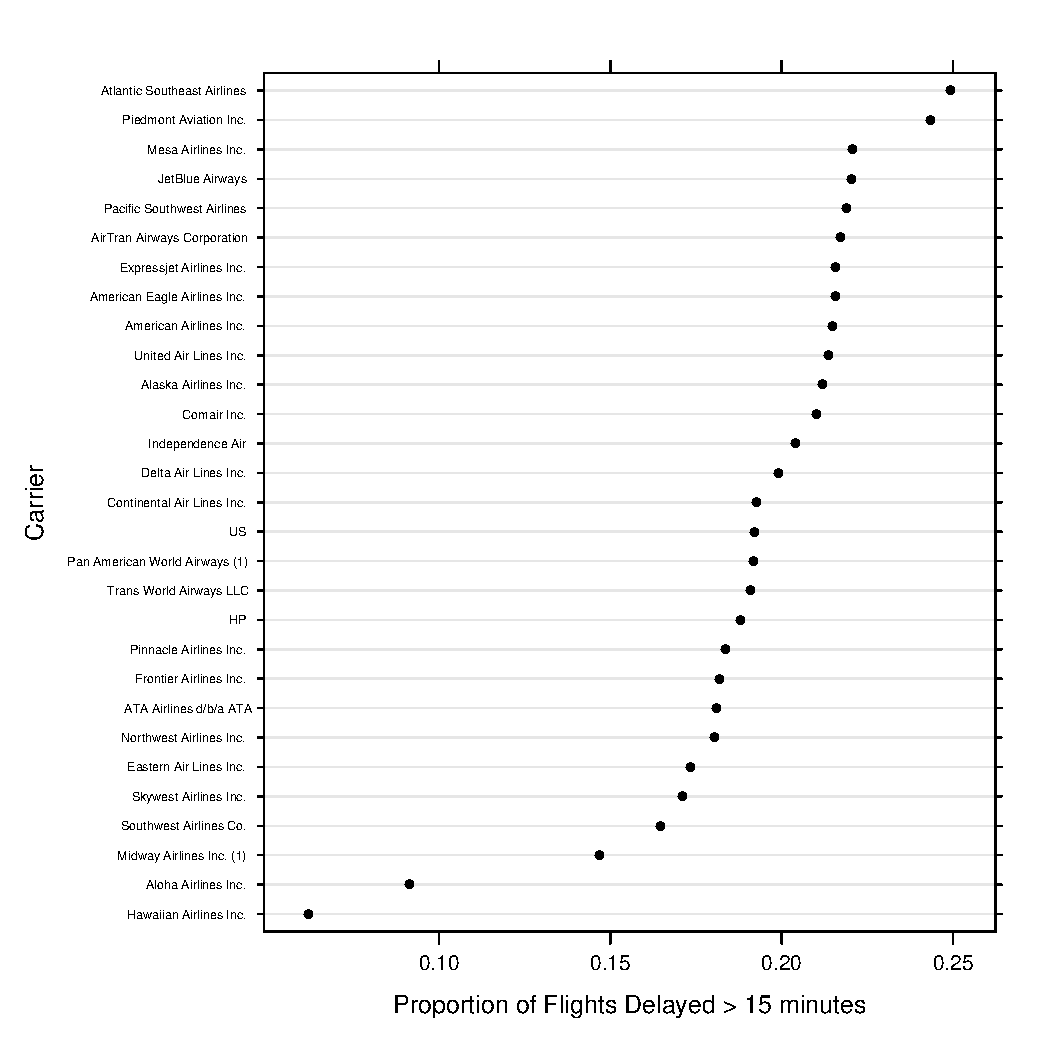
\includegraphics{carrdelay.pdf}
\caption{Proportion of flights delayed by carrier. Compare this with the previous graph.}\end{figure}


\subsection{Busy Routes}
\label{airline:busy-routes}
Which are busy the routes? A simple first approach (for display purposed) is to
create a frequency table for the unordered pair \emph{(i,j)} where \emph{i} and \emph{j} are
distinct airport codes. Displays this over the US map.

\begin{Verbatim}[commandchars=\\\{\},numbers=left,firstnumber=1,stepnumber=1]
map \PYG{o}{\textless{}-} expression\PYG{p}{(}\PYG{p}{\PYGZob{}}
  a \PYG{o}{\textless{}-} do.call\PYG{p}{(}\PYG{l+s}{"}\PYG{l+s}{rbind"}\PYG{p}{,}map.values\PYG{p}{)}
  y \PYG{o}{\textless{}-} table\PYG{p}{(}apply\PYG{p}{(}a\PYG{p}{[}\PYG{p}{,}c\PYG{p}{(}\PYG{l+s}{"}\PYG{l+s}{origin"}\PYG{p}{,}\PYG{l+s}{"}\PYG{l+s}{dest"}\PYG{p}{)}\PYG{p}{]}\PYG{p}{,}\PYG{l+m}{1}\PYG{p}{,}\PYG{k+kr}{function}\PYG{p}{(}r\PYG{p}{)}\PYG{p}{\PYGZob{}}
    paste\PYG{p}{(}sort\PYG{p}{(}r\PYG{p}{)}\PYG{p}{,}collapse\PYG{o}{=}\PYG{l+s}{"}\PYG{l+s}{,"}\PYG{p}{)}
  \PYG{p}{\PYGZcb{}}\PYG{p}{)}\PYG{p}{)}
  \PYG{k+kr}{for}\PYG{p}{(}i in \PYG{l+m}{1}:length\PYG{p}{(}y\PYG{p}{)}\PYG{p}{)}\PYG{p}{\PYGZob{}}
    p \PYG{o}{\textless{}-} strsplit\PYG{p}{(}names\PYG{p}{(}y\PYG{p}{)}\PYG{p}{[}\PYG{p}{[}i\PYG{p}{]}\PYG{p}{]}\PYG{p}{,}\PYG{l+s}{"}\PYG{l+s}{,"}\PYG{p}{)}\PYG{p}{[}\PYG{p}{[}\PYG{l+m}{1}\PYG{p}{]}\PYG{p}{]}
    rhcollect\PYG{p}{(}p\PYG{p}{,}y\PYG{p}{[}\PYG{p}{[}\PYG{l+m}{1}\PYG{p}{]}\PYG{p}{]}\PYG{p}{)}
  \PYG{p}{\PYGZcb{}}
\PYG{p}{\PYGZcb{}}\PYG{p}{)}
reduce \PYG{o}{\textless{}-} expression\PYG{p}{(}
    pre\PYG{o}{=}\PYG{p}{\PYGZob{}}sums \PYG{o}{\textless{}-} \PYG{l+m}{0}\PYG{p}{\PYGZcb{}}\PYG{p}{,}
    reduce \PYG{o}{=} \PYG{p}{\PYGZob{}}sums \PYG{o}{\textless{}-} sums\PYG{o}{+}sum\PYG{p}{(}unlist\PYG{p}{(}reduce.values\PYG{p}{)}\PYG{p}{)}\PYG{p}{\PYGZcb{}}\PYG{p}{,}
    post \PYG{o}{=} \PYG{p}{\PYGZob{}} rhcollect\PYG{p}{(}reduce.key\PYG{p}{,} sums\PYG{p}{)} \PYG{p}{\PYGZcb{}}
    \PYG{p}{)}
mapred \PYG{o}{\textless{}-} list\PYG{p}{(}\PYG{p}{)}
mapred\PYG{p}{\$}rhipe\PYGZus{}map\PYGZus{}buff\PYGZus{}size \PYG{o}{\textless{}-} \PYG{l+m}{5}
mapred\PYG{p}{\$}mapred.job.priority\PYG{o}{=}\PYG{l+s}{"}\PYG{l+s}{VERY\PYGZus{}LOW"}
z \PYG{o}{\textless{}-} rhmr\PYG{p}{(}map\PYG{o}{=}map\PYG{p}{,}reduce\PYG{o}{=}reduce\PYG{p}{,}combiner\PYG{o}{=}\PYG{k+kc}{TRUE}\PYG{p}{,}inout\PYG{o}{=}c\PYG{p}{(}\PYG{l+s}{"}\PYG{l+s}{sequence"}\PYG{p}{,}\PYG{l+s}{"}\PYG{l+s}{sequence"}\PYG{p}{)}
          \PYG{p}{,}ifolder\PYG{o}{=}\PYG{l+s}{"}\PYG{l+s}{/airline/blocks/"}\PYG{p}{,}ofolder\PYG{o}{=}\PYG{l+s}{"}\PYG{l+s}{/airline/ijjoin"}
          \PYG{p}{,}mapred\PYG{o}{=}mapred\PYG{p}{)}
z\PYG{o}{=}rhex\PYG{p}{(}z\PYG{p}{)}

\PYG{c+c1}{\#\#Merge results}
b\PYG{o}{=}rhread\PYG{p}{(}\PYG{l+s}{"}\PYG{l+s}{/airline/ijjoin"}\PYG{p}{)}
y \PYG{o}{\textless{}-} do.call\PYG{p}{(}\PYG{l+s}{"}\PYG{l+s}{rbind"}\PYG{p}{,}lapply\PYG{p}{(}b\PYG{p}{,}\PYG{l+s}{"}\PYG{l+s}{[["}\PYG{p}{,}\PYG{l+m}{1}\PYG{p}{)}\PYG{p}{)}
results \PYG{o}{\textless{}-} data.frame\PYG{p}{(}a\PYG{o}{=}y\PYG{p}{[}\PYG{p}{,}\PYG{l+m}{1}\PYG{p}{]}\PYG{p}{,}b\PYG{o}{=}y\PYG{p}{[}\PYG{p}{,}\PYG{l+m}{2}\PYG{p}{]}\PYG{p}{,}count\PYG{o}{=}
           do.call\PYG{p}{(}\PYG{l+s}{"}\PYG{l+s}{rbind"}\PYG{p}{,}lapply\PYG{p}{(}b\PYG{p}{,}\PYG{l+s}{"}\PYG{l+s}{[["}\PYG{p}{,}\PYG{l+m}{2}\PYG{p}{)}\PYG{p}{)}\PYG{p}{,}stringsAsFactors\PYG{o}{=}\PYG{k+kc}{FALSE}\PYG{p}{)}
results \PYG{o}{\textless{}-} results\PYG{p}{[}order\PYG{p}{(}results\PYG{p}{\$}count\PYG{p}{,}decreasing\PYG{o}{=}\PYG{k+kc}{TRUE}\PYG{p}{)}\PYG{p}{,}\PYG{p}{]}
results\PYG{p}{\$}cumprop \PYG{o}{\textless{}-} cumsum\PYG{p}{(}results\PYG{p}{\$}count\PYG{p}{)}\PYG{o}{/}sum\PYG{p}{(}results\PYG{p}{\$}count\PYG{p}{)}
a.lat \PYG{o}{\textless{}-} t\PYG{p}{(}sapply\PYG{p}{(}results\PYG{p}{\$}a\PYG{p}{,}\PYG{k+kr}{function}\PYG{p}{(}r\PYG{p}{)}\PYG{p}{\PYGZob{}}
  ap\PYG{p}{[}ap\PYG{p}{\$}iata\PYG{o}{==}r\PYG{p}{,}c\PYG{p}{(}\PYG{l+s}{'}\PYG{l+s}{lat'}\PYG{p}{,}\PYG{l+s}{'}\PYG{l+s}{long'}\PYG{p}{)}\PYG{p}{]}
\PYG{p}{\PYGZcb{}}\PYG{p}{)}\PYG{p}{)}
results\PYG{p}{\$}a.lat \PYG{o}{\textless{}-} unlist\PYG{p}{(}a.lat\PYG{p}{[}\PYG{p}{,}\PYG{l+s}{'}\PYG{l+s}{lat'}\PYG{p}{]}\PYG{p}{)}
results\PYG{p}{\$}a.long \PYG{o}{\textless{}-} unlist\PYG{p}{(}a.lat\PYG{p}{[}\PYG{p}{,}\PYG{l+s}{'}\PYG{l+s}{long'}\PYG{p}{]}\PYG{p}{)}
b.lat \PYG{o}{\textless{}-} t\PYG{p}{(}sapply\PYG{p}{(}results\PYG{p}{\$}b\PYG{p}{,}\PYG{k+kr}{function}\PYG{p}{(}r\PYG{p}{)}\PYG{p}{\PYGZob{}}
  ap\PYG{p}{[}ap\PYG{p}{\$}iata\PYG{o}{==}r\PYG{p}{,}c\PYG{p}{(}\PYG{l+s}{'}\PYG{l+s}{lat'}\PYG{p}{,}\PYG{l+s}{'}\PYG{l+s}{long'}\PYG{p}{)}\PYG{p}{]}
\PYG{p}{\PYGZcb{}}\PYG{p}{)}\PYG{p}{)}
b.lat\PYG{p}{[}\PYG{l+s}{"}\PYG{l+s}{CBM"}\PYG{p}{,}\PYG{p}{]} \PYG{o}{\textless{}-} c\PYG{p}{(}\PYG{l+m}{0}\PYG{p}{,}\PYG{l+m}{0}\PYG{p}{)}
results\PYG{p}{\$}b.lat \PYG{o}{\textless{}-} unlist\PYG{p}{(}b.lat\PYG{p}{[}\PYG{p}{,}\PYG{l+s}{'}\PYG{l+s}{lat'}\PYG{p}{]}\PYG{p}{)}
results\PYG{p}{\$}b.long \PYG{o}{\textless{}-} unlist\PYG{p}{(}b.lat\PYG{p}{[}\PYG{p}{,}\PYG{l+s}{'}\PYG{l+s}{long'}\PYG{p}{]}\PYG{p}{)}

head\PYG{p}{(}results\PYG{p}{)}
   a   b  count     cumprop    a.lat     a.long    b.lat     b.long
\PYG{l+m}{1} ATL ORD \PYG{l+m}{145810} \PYG{l+m}{0.001637867} \PYG{l+m}{33.64044}  \PYG{l+m}{-84.42694} \PYG{l+m}{41.97960}  \PYG{l+m}{-87.90446}
\PYG{l+m}{2} LAS LAX \PYG{l+m}{140722} \PYG{l+m}{0.003218581} \PYG{l+m}{36.08036} \PYG{l+m}{-115.15233} \PYG{l+m}{33.94254} \PYG{l+m}{-118.40807}
\PYG{l+m}{3} DEN DFW \PYG{l+m}{140258} \PYG{l+m}{0.004794083} \PYG{l+m}{39.85841} \PYG{l+m}{-104.66700} \PYG{l+m}{32.89595}  \PYG{l+m}{-97.03720}
\PYG{l+m}{4} LAX SFO \PYG{l+m}{139427} \PYG{l+m}{0.006360250} \PYG{l+m}{33.94254} \PYG{l+m}{-118.40807} \PYG{l+m}{37.61900} \PYG{l+m}{-122.37484}
\PYG{l+m}{5} DFW IAH \PYG{l+m}{137004} \PYG{l+m}{0.007899200} \PYG{l+m}{32.89595}  \PYG{l+m}{-97.03720} \PYG{l+m}{29.98047}  \PYG{l+m}{-95.33972}
\PYG{l+m}{6} DTW ORD \PYG{l+m}{135772} \PYG{l+m}{0.009424311} \PYG{l+m}{42.21206}  \PYG{l+m}{-83.34884} \PYG{l+m}{41.97960}  \PYG{l+m}{-87.90446}
\end{Verbatim}

Using the above data, the following figure draws lines from ORD (Chicago) to
other destinations. The black points are the airports that handle 90\% of the
total air traffic volume. The grey points are the remaining airports. The
flights from Chicago (ORD) are color coded based on volume carried e.g. red
implies those routes carry the top 25\% of traffic in/out of ORD.
\begin{figure}[htbp]
\centering

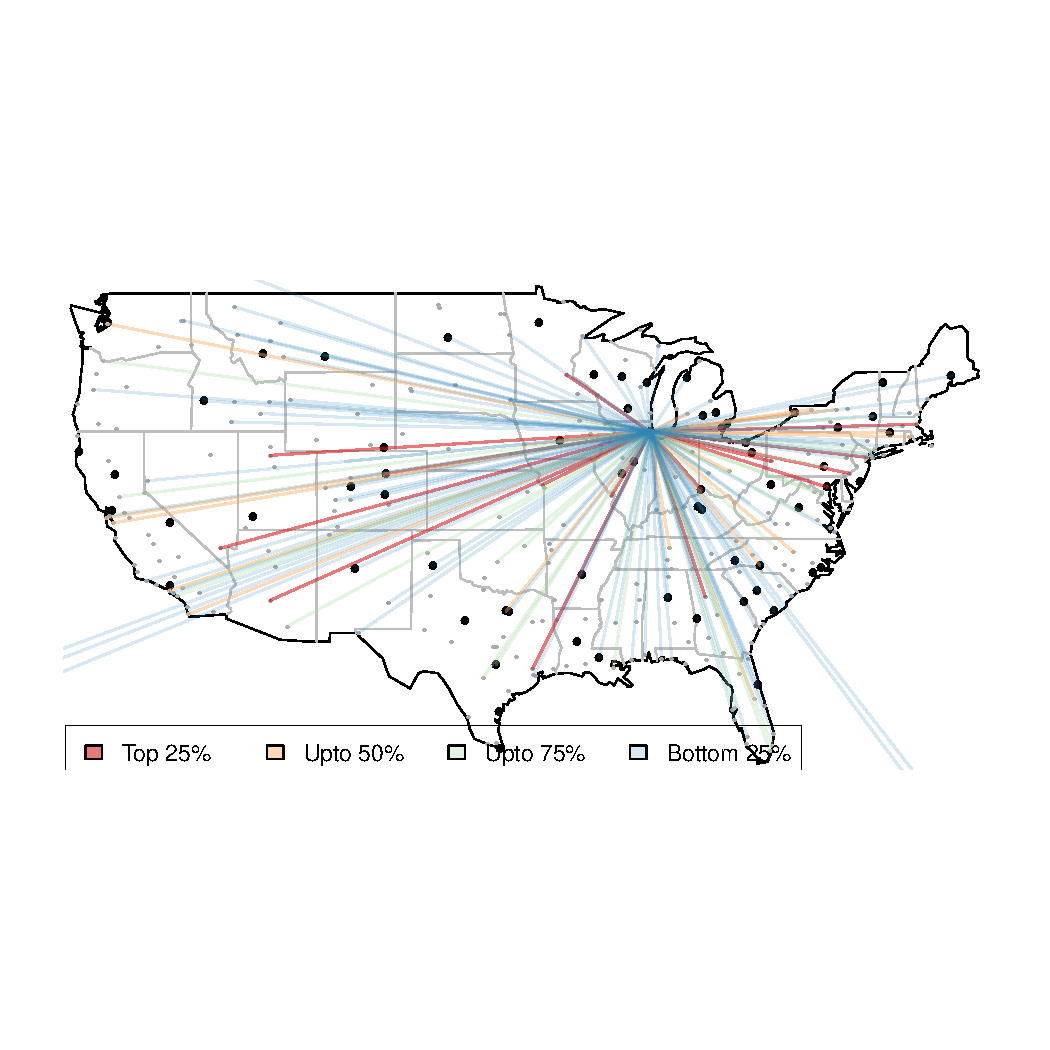
\includegraphics{flightord.pdf}
\caption{Flights in and out of Chicago color coded by \% cumulative contribution.}\end{figure}


\section{Streaming Data?}
\label{airline:id6}\label{airline:streaming-data}\index{orderby}\index{streaming}\index{partitioner}
Some algorithms are left associative in their operands
$t_1,t_2,\ldots,t_n$ but not commutative. For example a streaming update
algorithm that computes the inter-arrival times of time series data for
different levels of a categorical variable. That is, the triangular series
$t_{k,1},t_{k,2},\ldots,t_{k,n_k}$ where \emph{k} takes the levels of a
categorical variable \emph{C} (which takes the values $1,2,3,\ldots,m$). The
input are pairs $(i,j), i \in \{1,2,\ldots,m\}, j \in \{t_{ik}\}$
. In the following code, the data structure \emph{F} is updated with the
\emph{datastructure} contained in the values (see the map). The \emph{datastructures}
are indexed in time by the \emph{timepoint} - they need to be sent to the reducer
(for a given level of the categorical variable \emph{catlevel}) in time order. Thus
the map sends the pair \code{(catlevel, timepoint)} as the key. By using the
\code{part} parameter (see line 39) \emph{all} the data structures associated with the \code{catlevel}
are sent to the same R reduce process. This is vital since all the component
R expressions in the reduce are run in the same process and namespace. To
preserve numeric ordering we insist on the special map output key class (see
line 38). With this special key class, we cannot have a map output format.
In the reduce, the setup expression \code{redsetup} is run upon R startup (the
process assigned to several keys and their associated values). Then for each new
intermediate key \code{(catlevel, timepoint)}, it runs the \code{pre}, \code{reduce} and
\code{post}. The lack of a \code{post} is because we have exactly one intermediate
value for a given key (assuming the time points for a category are unique).
The \code{redclose} expression is run when all keys and values have been processed
by the reducer and R is about to quit.

\begin{Verbatim}[commandchars=\\\{\},numbers=left,firstnumber=1,stepnumber=1]
map \PYG{o}{\textless{}-} expression\PYG{p}{(}\PYG{p}{\PYGZob{}}
  lapply\PYG{p}{(}seq\PYGZus{}along\PYG{p}{(}map.values\PYG{p}{)}\PYG{p}{,}\PYG{k+kr}{function}\PYG{p}{(}r\PYG{p}{)}\PYG{p}{\PYGZob{}}
    catlevel \PYG{o}{\textless{}-} map.keys\PYG{p}{[}\PYG{p}{[}r\PYG{p}{]}\PYG{p}{]} \PYG{c+c1}{\#numeric}
    timepoint \PYG{o}{\textless{}-} map.values\PYG{p}{[}\PYG{p}{[}r\PYG{p}{]}\PYG{p}{]}\PYG{p}{\$}timepoint \PYG{c+c1}{\#numeric}
    datastructure \PYG{o}{\textless{}-} map.values\PYG{p}{[}\PYG{p}{[}r\PYG{p}{]}\PYG{p}{]}\PYG{p}{\$}data
    key \PYG{o}{\textless{}-} c\PYG{p}{(}catlevel\PYG{p}{,}timepoint\PYG{p}{)}
    rhcollect\PYG{p}{(}key\PYG{p}{,}datastructure\PYG{p}{)}
  \PYG{p}{\PYGZcb{}}\PYG{p}{)}
\PYG{p}{\PYGZcb{}}\PYG{p}{)}
redsetup \PYG{o}{\textless{}-} expression\PYG{p}{(}\PYG{p}{\PYGZob{}}
  currentkey \PYG{o}{\textless{}-} \PYG{k+kc}{NULL}
\PYG{p}{\PYGZcb{}}\PYG{p}{)}
reduce \PYG{o}{\textless{}-} expression\PYG{p}{(}
    pre\PYG{o}{=}\PYG{p}{\PYGZob{}}
      catlevel \PYG{o}{\textless{}-} reduce.key\PYG{p}{[}\PYG{l+m}{1}\PYG{p}{]}
      time \PYG{o}{\textless{}-} reduce.key\PYG{p}{[}\PYG{l+m}{2}\PYG{p}{]}
      \PYG{k+kr}{if}\PYG{p}{(}!identical\PYG{p}{(}catlevel\PYG{p}{,}currentkey\PYG{p}{)}\PYG{p}{)}\PYG{p}{\PYGZob{}}
        \PYG{c+c1}{\#\# new categorical level}
        \PYG{c+c1}{\#\# so finalize the computation for}
        \PYG{c+c1}{\#\# the previous level e.g. use rhcollect}
        \PYG{k+kr}{if}\PYG{p}{(}!identical\PYG{p}{(}currentkey\PYG{p}{,}\PYG{k+kc}{NULL}\PYG{p}{)}\PYG{p}{)}
          FINALIZE\PYG{p}{(}\PYG{k+kVariable}{F}\PYG{p}{)}
        \PYG{c+c1}{\#\# store current categorical level}
        currentkey \PYG{o}{\textless{}-} catlevel
        \PYG{c+c1}{\#\# initialize computation for new level}
        INITIALIZE\PYG{p}{(}\PYG{k+kVariable}{F}\PYG{p}{)}
      \PYG{p}{\PYGZcb{}}
    \PYG{p}{\PYGZcb{}}\PYG{p}{,}
    reduce\PYG{o}{=}\PYG{p}{\PYGZob{}}
      \PYG{k+kVariable}{F} \PYG{o}{\textless{}-} UPDATE\PYG{p}{(}\PYG{k+kVariable}{F}\PYG{p}{,} reduce.values\PYG{p}{[}\PYG{p}{[}\PYG{l+m}{1}\PYG{p}{]}\PYG{p}{]}\PYG{p}{)}
    \PYG{p}{\PYGZcb{}}\PYG{p}{)}
redclose \PYG{o}{\textless{}-} expression\PYG{p}{(}\PYG{p}{\PYGZob{}}
  \PYG{c+c1}{\#\# need to run this, otherwise the last catlevel}
  \PYG{c+c1}{\#\# will not get finalized}
 FINALIZE\PYG{p}{(}\PYG{k+kVariable}{F}\PYG{p}{)}
\PYG{p}{\PYGZcb{}}\PYG{p}{)}
rhmr\PYG{p}{(}\PYG{l+m}{.}\PYG{l+m}{.}\PYG{l+m}{.}\PYG{p}{,} combiner\PYG{o}{=}\PYG{k+kc}{FALSE}\PYG{p}{,}setup\PYG{o}{=}list\PYG{p}{(}reduce\PYG{o}{=}redsetup\PYG{p}{)}\PYG{p}{,}cleanup\PYG{o}{=}list\PYG{p}{(}reduce\PYG{o}{=}redclose\PYG{p}{)}\PYG{p}{,}
     orderby\PYG{o}{=}\PYG{l+s}{"}\PYG{l+s}{numeric"}\PYG{p}{,}
     part\PYG{o}{=}list\PYG{p}{(}lims\PYG{o}{=}\PYG{l+m}{1}\PYG{p}{,}type\PYG{o}{=}\PYG{l+s}{'}\PYG{l+s}{numeric'}\PYG{p}{)}\PYG{p}{)}
\end{Verbatim}


\section{Simple Debugging}
\label{airline:simple-debugging}\index{debugging}\index{tryCatch}
Consider the example code used to compute the delay quantiles by month (see
\hyperref[airline:delay-quantiles-by-month]{\emph{Delay Quantiles By Month}} ). We can use \code{tryCatch} for some simple
debugging. See the error in line 7, there is no such variable \code{isdelayed}

\begin{Verbatim}[commandchars=\\\{\},numbers=left,firstnumber=1,stepnumber=1]
map \PYG{o}{\textless{}-} expression\PYG{p}{(}\PYG{p}{\PYGZob{}}
  tryCatch\PYG{p}{(}\PYG{p}{\PYGZob{}}
    a \PYG{o}{\textless{}-} do.call\PYG{p}{(}\PYG{l+s}{"}\PYG{l+s}{rbind"}\PYG{p}{,}map.values\PYG{p}{)}
    a\PYG{p}{\$}delay.sec \PYG{o}{\textless{}-} as.vector\PYG{p}{(}a\PYG{p}{[}\PYG{p}{,}\PYG{l+s}{'}\PYG{l+s}{arrive'}\PYG{p}{]}\PYG{p}{)}\PYG{o}{-}as.vector\PYG{p}{(}a\PYG{p}{[}\PYG{p}{,}\PYG{l+s}{'}\PYG{l+s}{sarrive'}\PYG{p}{]}\PYG{p}{)}
    a \PYG{o}{\textless{}-} a\PYG{p}{[}!is.na\PYG{p}{(}a\PYG{p}{\$}delay.sec\PYG{p}{)}\PYG{p}{,}\PYG{p}{]}
    a\PYG{p}{\$}isdelayed \PYG{o}{\textless{}-} sapply\PYG{p}{(}a\PYG{p}{\$}delay.sec\PYG{p}{,}\PYG{k+kr}{function}\PYG{p}{(}r\PYG{p}{)} \PYG{k+kr}{if}\PYG{p}{(}r\PYG{o}{\textgreater{}=}\PYG{l+m}{900}\PYG{p}{)} \PYG{k+kc}{TRUE} \PYG{k+kr}{else} \PYG{k+kc}{FALSE}\PYG{p}{)}
    a \PYG{o}{\textless{}-} a\PYG{p}{[}isdelayed\PYG{o}{==}\PYG{k+kc}{TRUE}\PYG{p}{,}\PYG{p}{]} \PYG{c+c1}{\#\# only look at delays greater than 15 minutes}
    apply\PYG{p}{(}a\PYG{p}{[}\PYG{p}{,}c\PYG{p}{(}\PYG{l+s}{'}\PYG{l+s}{month'}\PYG{p}{,}\PYG{l+s}{'}\PYG{l+s}{delay.sec'}\PYG{p}{)}\PYG{p}{]}\PYG{p}{,}\PYG{l+m}{1}\PYG{p}{,}\PYG{k+kr}{function}\PYG{p}{(}r\PYG{p}{)}\PYG{p}{\PYGZob{}}
      k \PYG{o}{\textless{}-} as.vector\PYG{p}{(}unlist\PYG{p}{(}r\PYG{p}{)}\PYG{p}{)}
      \PYG{k+kr}{if}\PYG{p}{(}!is.na\PYG{p}{(}k\PYG{p}{[}\PYG{l+m}{1}\PYG{p}{]}\PYG{p}{)}\PYG{p}{)} rhcollect\PYG{p}{(}k\PYG{p}{,}\PYG{l+m}{1}\PYG{p}{)} \PYG{c+c1}{\# ignore cases where month is missing}
    \PYG{p}{\PYGZcb{}}\PYG{p}{)}
  \PYG{p}{\PYGZcb{}}\PYG{p}{,}error\PYG{o}{=}\PYG{k+kr}{function}\PYG{p}{(}e\PYG{p}{)}\PYG{p}{\PYGZob{}}
    e\PYG{p}{\$}message \PYG{o}{\textless{}-} sprintf\PYG{p}{(}\PYG{l+s}{"}\PYG{l+s}{Input File:\%s\PYGZbs{}nAttempt ID:\%s\PYGZbs{}nR INFO:\%s"}\PYG{p}{,}
                 Sys.getenv\PYG{p}{(}\PYG{l+s}{"}\PYG{l+s}{mapred.input.file"}\PYG{p}{)}\PYG{p}{,}Sys.getenv\PYG{p}{(}\PYG{l+s}{"}\PYG{l+s}{mapred.task.id"}\PYG{p}{)}\PYG{p}{,}e\PYG{p}{\$}message\PYG{p}{)}
    stop\PYG{p}{(}e\PYG{p}{)} \PYG{c+c1}{\#\# WONT STOP OTHERWISE}
  \PYG{p}{\PYGZcb{}}\PYG{p}{)}
\PYG{p}{\PYGZcb{}}\PYG{p}{)}
  reduce \PYG{o}{\textless{}-} expression\PYG{p}{(}
    pre\PYG{o}{=}\PYG{p}{\PYGZob{}}sums \PYG{o}{\textless{}-} \PYG{l+m}{0}\PYG{p}{\PYGZcb{}} \PYG{p}{,}
    reduce \PYG{o}{=} \PYG{p}{\PYGZob{}}sums \PYG{o}{\textless{}-} sums\PYG{o}{+}sum\PYG{p}{(}unlist\PYG{p}{(}reduce.values\PYG{p}{)}\PYG{p}{)}\PYG{p}{\PYGZcb{}}\PYG{p}{,}
    post \PYG{o}{=} \PYG{p}{\PYGZob{}} rhcollect\PYG{p}{(}reduce.key\PYG{p}{,} sums\PYG{p}{)} \PYG{p}{\PYGZcb{}}
    \PYG{p}{)}
mapred \PYG{o}{\textless{}-} list\PYG{p}{(}\PYG{p}{)}
mapred\PYG{p}{\$}rhipe\PYGZus{}map\PYGZus{}buff\PYGZus{}size \PYG{o}{\textless{}-} \PYG{l+m}{5}
z \PYG{o}{\textless{}-} rhmr\PYG{p}{(}map\PYG{o}{=}map\PYG{p}{,}reduce\PYG{o}{=}reduce\PYG{p}{,}combiner\PYG{o}{=}\PYG{k+kc}{TRUE}\PYG{p}{,}inout\PYG{o}{=}c\PYG{p}{(}\PYG{l+s}{"}\PYG{l+s}{sequence"}\PYG{p}{,}\PYG{l+s}{"}\PYG{l+s}{sequence"}\PYG{p}{)}
          \PYG{p}{,}ifolder\PYG{o}{=}\PYG{l+s}{"}\PYG{l+s}{/airline/blocks/"}\PYG{p}{,}ofolder\PYG{o}{=}\PYG{l+s}{"}\PYG{l+s}{/airline/quantiledelay"}
          \PYG{p}{,}mapred\PYG{o}{=}mapred\PYG{p}{)}
z\PYG{o}{=}rhex\PYG{p}{(}z\PYG{p}{)}
\end{Verbatim}

Produces a slew of errors like
\index{counter}
\begin{Verbatim}[commandchars=\\\{\},numbers=left,firstnumber=1,stepnumber=1]
\PYG{l+m}{10}\PYG{o}{/}\PYG{l+m}{08}\PYG{o}{/}\PYG{l+m}{04} \PYG{l+m}{00}:\PYG{l+m}{41}:\PYG{l+m}{20} INFO mapred.JobClient: Task Id : attempt\PYGZus{}201007281701\PYGZus{}0273\PYGZus{}m\PYGZus{}000023\PYGZus{}0\PYG{p}{,} Status : FAILED
java.io.IOException: MROutput\PYG{o}{/}MRErrThread failed:java.lang.RuntimeException:
R ERROR
\PYG{o}{==}\PYG{o}{==}\PYG{o}{==}\PYG{o}{=}
Error in \PYG{l+s+sb}{{}`[.data.frame{}`}\PYG{p}{(}a\PYG{p}{,} isdelayed \PYG{o}{==} \PYG{k+kc}{TRUE}\PYG{p}{,} \PYG{p}{)} : Input File:
Attempt ID:attempt\PYGZus{}201007281701\PYGZus{}0273\PYGZus{}m\PYGZus{}000023\PYGZus{}0
R INFO:object \PYG{l+s}{"}\PYG{l+s}{isdelayed"} not found
\end{Verbatim}

It can be very useful to provide such debugging messages since R itself doesn't
provide much help. Use this to provide context about variables, such printing
the first few rows of relevant data frames (if required). Moreover, some errors
don't come to the screen instead the job finishes successfully (but very quickly
since the R code is failing) but the error message is returned as a counter. The
splits succeed since Hadoop has finished sending its data to R and not listening
to for errors from the R code. Hence any errors sent from R do not trigger a
failure condition in Hadoop. This is a RHIPE design flaw. To compensate for
this, the errors are stored in the counter \emph{R\_ERROR}.

Unfortunately, RHIPE does not offer much in the way of debugging. To run jobs
locally that is, Hadoop will execute the job in a single thread on one computer,
set \code{mapred.job.tracker} to \emph{local} in the \code{mapred} argument of \code{rhmr}. In
this case, \code{shared.files} cannot be used and \code{copyFiles} will not work.
\phantomsection\label{texttransfirm:rhipeserialize}\index{textouput!transformations on text files}\index{textouput!subsets of text files}\index{textoutput!quoting text}\index{textoutput!separators for vectors}\index{rhipe\_string\_quote}\index{mapred.field.separator}\index{mapred.textoutputformat.usekey}

\chapter{Transforming Text Data}
\label{texttransfirm::doc}\label{texttransfirm:index-2}\label{texttransfirm:transforming-text-data}
This chapter builds on the \emph{Airline Dataset}. One foreseeable use of RHIPE is
to transform text data. For example,
\begin{enumerate}
\item {} 
Subset Southwest Airline and Delat Airways information to create a new set of text files, one with only Southwest and the other with Delta.

\item {} 
Transform the original text data to one with fewer columns and some transformed e.g. Airport Codes to full names.

\end{enumerate}

We'll cover both examples.
\index{partitioner}

\section{Subset}
\label{texttransfirm:subset}\label{texttransfirm:index-3}
The text data looks like

\begin{Verbatim}[commandchars=\\\{\}]
\PYG{l+m}{1987}\PYG{p}{,}\PYG{l+m}{10}\PYG{p}{,}\PYG{l+m}{23}\PYG{p}{,}\PYG{l+m}{5}\PYG{p}{,}\PYG{l+m}{1841}\PYG{p}{,}\PYG{l+m}{1750}\PYG{p}{,}\PYG{l+m}{2105}\PYG{p}{,}\PYG{l+m}{2005}\PYG{p}{,}PS\PYG{p}{,}\PYG{l+m}{1905}\PYG{p}{,}\PYG{k+kc}{NA}\PYG{p}{,}\PYG{l+m}{144}\PYG{p}{,}\PYG{l+m}{135}\PYG{p}{,}\PYG{k+kc}{NA}\PYG{p}{,}\PYG{l+m}{60}\PYG{p}{,}\PYG{l+m}{51}\PYG{p}{,}LAX\PYG{p}{,}SEA\PYG{p}{,}\PYG{l+m}{954}\PYG{p}{,}\PYG{k+kc}{NA}\PYG{p}{,}\PYG{k+kc}{NA}\PYG{p}{,}\PYG{l+m}{0}\PYG{p}{,}\PYG{k+kc}{NA}\PYG{p}{,}\PYG{l+m}{0}\PYG{p}{,}\PYG{l+m}{.}\PYG{l+m}{.}\PYG{l+m}{.}
\PYG{l+m}{1987}\PYG{p}{,}\PYG{l+m}{10}\PYG{p}{,}\PYG{l+m}{24}\PYG{p}{,}\PYG{l+m}{6}\PYG{p}{,}\PYG{l+m}{1752}\PYG{p}{,}\PYG{l+m}{1750}\PYG{p}{,}\PYG{l+m}{2010}\PYG{p}{,}\PYG{l+m}{2005}\PYG{p}{,}PS\PYG{p}{,}\PYG{l+m}{1905}\PYG{p}{,}\PYG{k+kc}{NA}\PYG{p}{,}\PYG{l+m}{138}\PYG{p}{,}\PYG{l+m}{135}\PYG{p}{,}\PYG{k+kc}{NA}\PYG{p}{,}\PYG{l+m}{5}\PYG{p}{,}\PYG{l+m}{2}\PYG{p}{,}LAX\PYG{p}{,}SEA\PYG{p}{,}\PYG{l+m}{954}\PYG{p}{,}\PYG{k+kc}{NA}\PYG{p}{,}\PYG{k+kc}{NA}\PYG{p}{,}\PYG{l+m}{0}\PYG{p}{,}\PYG{k+kc}{NA}\PYG{p}{,}\PYG{l+m}{0}\PYG{p}{,}\PYG{l+m}{.}\PYG{l+m}{.}\PYG{l+m}{.}
\PYG{l+m}{.}\PYG{l+m}{.}\PYG{l+m}{.}
\PYG{l+m}{.}\PYG{l+m}{.}\PYG{l+m}{.}
\end{Verbatim}

The carrier name is column 9. Southwest carrier code is \emph{WN}, Delta is \emph{DL}. Only those rows with column 9
equal to \emph{WN} or \emph{DL} will be saved.

\begin{Verbatim}[commandchars=\\\{\},numbers=left,firstnumber=1,stepnumber=1]
map \PYG{o}{\textless{}-} expression\PYG{p}{(}\PYG{p}{\PYGZob{}}
  \PYG{c+c1}{\#\# Each element of map.values is a line of text}
  \PYG{c+c1}{\#\# this needs to be tokenized and then combined}
  tkn \PYG{o}{\textless{}-} strsplit\PYG{p}{(}unlist\PYG{p}{(}map.values\PYG{p}{)}\PYG{p}{,}\PYG{l+s}{"}\PYG{l+s}{,"}\PYG{p}{)}
  text \PYG{o}{\textless{}-} do.call\PYG{p}{(}\PYG{l+s}{"}\PYG{l+s}{rbind"}\PYG{p}{,}tkn\PYG{p}{)}
  text \PYG{o}{\textless{}-} text\PYG{p}{[}text\PYG{p}{[}\PYG{p}{,}\PYG{l+m}{9}\PYG{p}{]} \PYG{o}{\%in\%} c\PYG{p}{(}\PYG{l+s}{"}\PYG{l+s}{WN"}\PYG{p}{,}\PYG{l+s}{"}\PYG{l+s}{DL"}\PYG{p}{)}\PYG{p}{,}\PYG{p}{,}drop\PYG{o}{=}\PYG{k+kc}{FALSE}\PYG{p}{]}
  \PYG{k+kr}{if}\PYG{p}{(}nrow\PYG{p}{(}text\PYG{p}{)}\PYG{o}{\textgreater{}}\PYG{l+m}{0}\PYG{p}{)} apply\PYG{p}{(}text\PYG{p}{,}\PYG{l+m}{1}\PYG{p}{,} \PYG{k+kr}{function}\PYG{p}{(}r\PYG{p}{)} rhcollect\PYG{p}{(}r\PYG{p}{[}\PYG{l+m}{9}\PYG{p}{]}\PYG{p}{,} r\PYG{p}{)}\PYG{p}{)}
\PYG{p}{\PYGZcb{}}\PYG{p}{)}
\end{Verbatim}

\code{rhcollect} requires both a key and value but we have no need for the key. So
NULL is given as the key argument and \emph{mapred.textoutputformat.usekey} is set to
FALSE so that the key is not written to disk. RHIPE quotes strings, which we do
not want (nothing is quoted), so \emph{rhipe\_string\_quote} is set to
`' and \emph{mapred.field.separator} is  ``,'' since the original data is comma separated.
A partitioner is used to send all the Southwest flights to one file and Delta to another.

\begin{Verbatim}[commandchars=\\\{\},numbers=left,firstnumber=1,stepnumber=1]
z \PYG{o}{\textless{}-} rhmr\PYG{p}{(}map\PYG{o}{=}map\PYG{p}{,}ifolder\PYG{o}{=}\PYG{l+s}{"}\PYG{l+s}{/airline/data/2005.csv"}\PYG{p}{,}ofolder\PYG{o}{=}\PYG{l+s}{"}\PYG{l+s}{/airline/southdelta"}\PYG{p}{,}
          \PYG{p}{,}inout\PYG{o}{=}c\PYG{p}{(}\PYG{l+s}{"}\PYG{l+s}{text"}\PYG{p}{,}\PYG{l+s}{"}\PYG{l+s}{text"}\PYG{p}{)}\PYG{p}{,}orderby\PYG{o}{=}\PYG{l+s}{"}\PYG{l+s}{char"}\PYG{p}{,}
          part\PYG{o}{=}list\PYG{p}{(}lims\PYG{o}{=}\PYG{l+m}{1}\PYG{p}{,}type\PYG{o}{=}\PYG{l+s}{"}\PYG{l+s}{string"}\PYG{p}{)}\PYG{p}{,}
          mapred\PYG{o}{=}list\PYG{p}{(}
           mapred.reduce.tasks\PYG{o}{=}\PYG{l+m}{2}\PYG{p}{,}
            rhipe\PYGZus{}string\PYGZus{}quote\PYG{o}{=}\PYG{l+s}{'}\PYG{l+s}{'}\PYG{p}{,}
            mapred.field.separator\PYG{o}{=}\PYG{l+s}{"}\PYG{l+s}{,"}\PYG{p}{,}
            mapred.textoutputformat.usekey\PYG{o}{=}\PYG{k+kc}{FALSE}\PYG{p}{)}\PYG{p}{)}
rhex\PYG{p}{(}z\PYG{p}{)}
\end{Verbatim}

The output, in one file is

\begin{Verbatim}[commandchars=\\\{\}]
\PYG{l+m}{2005}\PYG{p}{,}\PYG{l+m}{1}\PYG{p}{,}\PYG{l+m}{5}\PYG{p}{,}\PYG{l+m}{3}\PYG{p}{,}\PYG{l+m}{1850}\PYG{p}{,}\PYG{l+m}{1850}\PYG{p}{,}\PYG{l+m}{2208}\PYG{p}{,}\PYG{l+m}{2025}\PYG{p}{,}WN\PYG{p}{,}\PYG{l+m}{791}\PYG{p}{,}N404\PYG{p}{,}\PYG{l+m}{258}\PYG{p}{,}\PYG{l+m}{155}\PYG{p}{,}\PYG{l+m}{207}\PYG{p}{,}\PYG{l+m}{103}\PYG{p}{,}\PYG{l+m}{0}\PYG{p}{,}BDL\PYG{p}{,}\PYG{l+m}{.}\PYG{l+m}{.}\PYG{l+m}{.}
\PYG{l+m}{2005}\PYG{p}{,}\PYG{l+m}{1}\PYG{p}{,}\PYG{l+m}{5}\PYG{p}{,}\PYG{l+m}{3}\PYG{p}{,}\PYG{l+m}{810}\PYG{p}{,}\PYG{l+m}{810}\PYG{p}{,}\PYG{l+m}{1010}\PYG{p}{,}\PYG{l+m}{940}\PYG{p}{,}WN\PYG{p}{,}\PYG{l+m}{824}\PYG{p}{,}N784\PYG{p}{,}\PYG{l+m}{180}\PYG{p}{,}\PYG{l+m}{150}\PYG{p}{,}\PYG{l+m}{155}\PYG{p}{,}\PYG{l+m}{30}\PYG{p}{,}\PYG{l+m}{0}\PYG{p}{,}BDL\PYG{p}{,}\PYG{l+m}{.}\PYG{l+m}{.}\PYG{l+m}{.}
\PYG{l+m}{2005}\PYG{p}{,}\PYG{l+m}{1}\PYG{p}{,}\PYG{l+m}{5}\PYG{p}{,}\PYG{l+m}{3}\PYG{p}{,}\PYG{l+m}{1430}\PYG{p}{,}\PYG{l+m}{1325}\PYG{p}{,}\PYG{l+m}{1559}\PYG{p}{,}\PYG{l+m}{1435}\PYG{p}{,}WN\PYG{p}{,}\PYG{l+m}{317}\PYG{p}{,}N306SW\PYG{p}{,}\PYG{l+m}{89}\PYG{p}{,}\PYG{l+m}{70}\PYG{p}{,}\PYG{l+m}{61}\PYG{p}{,}\PYG{l+m}{84}\PYG{p}{,}\PYG{l+m}{65}\PYG{p}{,}BDL\PYG{p}{,}\PYG{l+m}{.}\PYG{l+m}{.}\PYG{l+m}{.}
\PYG{l+m}{2005}\PYG{p}{,}\PYG{l+m}{1}\PYG{p}{,}\PYG{l+m}{5}\PYG{p}{,}\PYG{l+m}{3}\PYG{p}{,}\PYG{l+m}{705}\PYG{p}{,}\PYG{l+m}{705}\PYG{p}{,}\PYG{l+m}{830}\PYG{p}{,}\PYG{l+m}{815}\PYG{p}{,}WN\PYG{p}{,}\PYG{l+m}{472}\PYG{p}{,}N772\PYG{p}{,}\PYG{l+m}{85}\PYG{p}{,}\PYG{l+m}{70}\PYG{p}{,}\PYG{l+m}{57}\PYG{p}{,}\PYG{l+m}{15}\PYG{p}{,}\PYG{l+m}{0}\PYG{p}{,}BDL\PYG{p}{,}\PYG{l+m}{.}\PYG{l+m}{.}\PYG{l+m}{.}
\end{Verbatim}

and the other

\begin{Verbatim}[commandchars=\\\{\}]
\PYG{l+m}{2005}\PYG{p}{,}\PYG{l+m}{12}\PYG{p}{,}\PYG{l+m}{22}\PYG{p}{,}\PYG{l+m}{4}\PYG{p}{,}\PYG{l+m}{1652}\PYG{p}{,}\PYG{l+m}{1655}\PYG{p}{,}\PYG{l+m}{1815}\PYG{p}{,}\PYG{l+m}{1837}\PYG{p}{,}DL\PYG{p}{,}\PYG{l+m}{901}\PYG{p}{,}N109DL\PYG{p}{,}\PYG{l+m}{.}\PYG{l+m}{.}\PYG{l+m}{.}
\PYG{l+m}{2005}\PYG{p}{,}\PYG{l+m}{12}\PYG{p}{,}\PYG{l+m}{22}\PYG{p}{,}\PYG{l+m}{4}\PYG{p}{,}\PYG{l+m}{1825}\PYG{p}{,}\PYG{l+m}{1825}\PYG{p}{,}\PYG{l+m}{1858}\PYG{p}{,}\PYG{l+m}{1848}\PYG{p}{,}DL\PYG{p}{,}\PYG{l+m}{902}\PYG{p}{,}N932DL\PYG{p}{,}\PYG{l+m}{.}\PYG{l+m}{.}\PYG{l+m}{.}
\PYG{l+m}{2005}\PYG{p}{,}\PYG{l+m}{12}\PYG{p}{,}\PYG{l+m}{22}\PYG{p}{,}\PYG{l+m}{4}\PYG{p}{,}\PYG{l+m}{1507}\PYG{p}{,}\PYG{l+m}{1511}\PYG{p}{,}\PYG{l+m}{1641}\PYG{p}{,}\PYG{l+m}{1649}\PYG{p}{,}DL\PYG{p}{,}\PYG{l+m}{903}\PYG{p}{,}N306DL\PYG{p}{,}\PYG{l+m}{.}\PYG{l+m}{.}\PYG{l+m}{.}
\end{Verbatim}


\section{Transformations}
\label{texttransfirm:transformations}
Convert each airport codes to their name equivalent. Airport codes can be found at the \href{http://stat-computing.org/dataexpo/2009/the-data.html}{JSM website} . When working with massive data, repeatedly used operations need to be as fast as possible.
Thus we will save the airport code to airport name as a hash table using the \code{new.env} function.
Airport codes (origin and destination) are in columns 17 and 18. The \code{setup} expression loads this
data set and creates a function that does the mapping.

\begin{Verbatim}[commandchars=\\\{\},numbers=left,firstnumber=1,stepnumber=1]
airport \PYG{o}{\textless{}-} read.table\PYG{p}{(}\PYG{l+s}{"}\PYG{l+s}{\textasciitilde{}/tmp/airports.csv"}\PYG{p}{,}sep\PYG{o}{=}\PYG{l+s}{"}\PYG{l+s}{,"}\PYG{p}{,}header\PYG{o}{=}\PYG{k+kc}{TRUE}\PYG{p}{,}stringsAsFactors\PYG{o}{=}\PYG{k+kc}{FALSE}\PYG{p}{)}
aton \PYG{o}{\textless{}-} new.env\PYG{p}{(}\PYG{p}{)}
\PYG{k+kr}{for}\PYG{p}{(}i in \PYG{l+m}{1}:nrow\PYG{p}{(}airport\PYG{p}{)}\PYG{p}{)}\PYG{p}{\PYGZob{}}
  aton\PYG{p}{[}\PYG{p}{[} airport\PYG{p}{[}i\PYG{p}{,}\PYG{l+s}{"}\PYG{l+s}{iata"}\PYG{p}{]} \PYG{p}{]}\PYG{p}{]} \PYG{o}{\textless{}-} list\PYG{p}{(}ap\PYG{o}{=}airport\PYG{p}{[}i\PYG{p}{,}\PYG{l+s}{"}\PYG{l+s}{airport"}\PYG{p}{]}\PYG{p}{,}latlong\PYG{o}{=}airport\PYG{p}{[}i\PYG{p}{,}c\PYG{p}{(}\PYG{l+s}{"}\PYG{l+s}{lat"}\PYG{p}{,}\PYG{l+s}{"}\PYG{l+s}{long"}\PYG{p}{)}\PYG{p}{]}\PYG{p}{)}
\PYG{p}{\PYGZcb{}}
rhsave\PYG{p}{(}aton\PYG{p}{,}file\PYG{o}{=}\PYG{l+s}{"}\PYG{l+s}{/tmp/airports.Rdata"}\PYG{p}{)}

setup \PYG{o}{\textless{}-} expression\PYG{p}{(}\PYG{p}{\PYGZob{}}
  load\PYG{p}{(}\PYG{l+s}{"}\PYG{l+s}{airports.Rdata"}\PYG{p}{)}
  co \PYG{o}{\textless{}-} \PYG{k+kr}{function}\PYG{p}{(}N\PYG{p}{)}\PYG{p}{\PYGZob{}}
    sapply\PYG{p}{(}text\PYG{p}{[}\PYG{p}{,}N\PYG{p}{]}\PYG{p}{,}\PYG{k+kr}{function}\PYG{p}{(}r\PYG{p}{)}\PYG{p}{\PYGZob{}}
      o \PYG{o}{\textless{}-} aton\PYG{p}{[}\PYG{p}{[} r\PYG{p}{[}\PYG{l+m}{1}\PYG{p}{]} \PYG{p}{]}\PYG{p}{]}\PYG{p}{\$}ap
      \PYG{k+kr}{if}\PYG{p}{(}is.null\PYG{p}{(}o\PYG{p}{)}\PYG{p}{)} \PYG{k+kc}{NA} \PYG{k+kr}{else} sprintf\PYG{p}{(}\PYG{l+s}{'}\PYG{l+s}{"\%s"'}\PYG{p}{,}o\PYG{p}{)}
    \PYG{p}{\PYGZcb{}}\PYG{p}{)}
  \PYG{p}{\PYGZcb{}}
\PYG{p}{\PYGZcb{}}\PYG{p}{)}
\end{Verbatim}

The map will use the \code{aton} dictionary to get the complete names which are quoted (in line 13 above).
Removing the \code{sprintf} makes it much faster.

\begin{Verbatim}[commandchars=\\\{\},numbers=left,firstnumber=1,stepnumber=1]
map \PYG{o}{\textless{}-} expression\PYG{p}{(}\PYG{p}{\PYGZob{}}
  tkn \PYG{o}{\textless{}-} strsplit\PYG{p}{(}unlist\PYG{p}{(}map.values\PYG{p}{)}\PYG{p}{,}\PYG{l+s}{"}\PYG{l+s}{,"}\PYG{p}{)}
  text \PYG{o}{\textless{}-} do.call\PYG{p}{(}\PYG{l+s}{"}\PYG{l+s}{rbind"}\PYG{p}{,}tkn\PYG{p}{)}
  text\PYG{p}{[}\PYG{p}{,}\PYG{l+m}{17}\PYG{p}{]} \PYG{o}{\textless{}-} co\PYG{p}{(}\PYG{l+m}{17}\PYG{p}{)}
  text\PYG{p}{[}\PYG{p}{,}\PYG{l+m}{18}\PYG{p}{]} \PYG{o}{\textless{}-} co\PYG{p}{(}\PYG{l+m}{18}\PYG{p}{)}
  apply\PYG{p}{(}text\PYG{p}{,}\PYG{l+m}{1}\PYG{p}{,}\PYG{k+kr}{function}\PYG{p}{(}r\PYG{p}{)}\PYG{p}{\PYGZob{}}
    rhcollect\PYG{p}{(}\PYG{k+kc}{NULL}\PYG{p}{,}r\PYG{p}{)}
  \PYG{p}{\PYGZcb{}}\PYG{p}{)}
\PYG{p}{\PYGZcb{}}\PYG{p}{)}

z \PYG{o}{\textless{}-} rhmr\PYG{p}{(}map\PYG{o}{=}map\PYG{p}{,}ifolder\PYG{o}{=}\PYG{l+s}{"}\PYG{l+s}{/airline/data/2005.csv"}\PYG{p}{,}ofolder\PYG{o}{=}\PYG{l+s}{"}\PYG{l+s}{/airline/transform"}\PYG{p}{,}
          \PYG{p}{,}inout\PYG{o}{=}c\PYG{p}{(}\PYG{l+s}{"}\PYG{l+s}{text"}\PYG{p}{,}\PYG{l+s}{"}\PYG{l+s}{text"}\PYG{p}{)}\PYG{p}{,}
          shared\PYG{o}{=}c\PYG{p}{(}\PYG{l+s}{"}\PYG{l+s}{/airport/airports.Rdata"}\PYG{p}{)}\PYG{p}{,}
          setup\PYG{o}{=}setup\PYG{p}{,}
          mapred\PYG{o}{=}list\PYG{p}{(}
            mapred.reduce.tasks\PYG{o}{=}\PYG{l+m}{0}\PYG{p}{,}
            rhipe\PYGZus{}string\PYGZus{}quote\PYG{o}{=}\PYG{l+s}{'}\PYG{l+s}{'}\PYG{p}{,}
            mapred.field.separator\PYG{o}{=}\PYG{l+s}{"}\PYG{l+s}{,"}\PYG{p}{,}
            mapred.textoutputformat.usekey\PYG{o}{=}\PYG{k+kc}{FALSE}\PYG{p}{)}\PYG{p}{)}
rhex\PYG{p}{(}z\PYG{p}{)}
\end{Verbatim}

and this gives us

\begin{Verbatim}[commandchars=\\\{\}]
\PYG{l+m}{1987}\PYG{p}{,}\PYG{l+m}{10}\PYG{p}{,}\PYG{l+m}{28}\PYG{p}{,}\PYG{l+m}{3}\PYG{p}{,}\PYG{k+kc}{NA}\PYG{p}{,}\PYG{l+m}{1945}\PYG{p}{,}\PYG{k+kc}{NA}\PYG{p}{,}\PYG{l+m}{2100}\PYG{p}{,}\PYG{l+m}{.}\PYG{l+m}{.}\PYG{l+m}{.}\PYG{p}{,}\PYG{l+s}{"}\PYG{l+s}{San Francisco International"}\PYG{p}{,}\PYG{l+s}{"}\PYG{l+s}{John Wayne /Orange Co,...}
\PYG{l+s}{1987,10,29,4,2025,1945,2141,2100,...,"}San Francisco International\PYG{l+s}{"}\PYG{l+s}{,"}John Wayne \PYG{o}{/}Orange Co\PYG{p}{,}\PYG{l+m}{.}\PYG{l+m}{.}\PYG{l+m}{.}
\PYG{l+m}{1987}\PYG{p}{,}\PYG{l+m}{10}\PYG{p}{,}\PYG{l+m}{30}\PYG{p}{,}\PYG{l+m}{5}\PYG{p}{,}\PYG{l+m}{1947}\PYG{p}{,}\PYG{l+m}{1945}\PYG{p}{,}\PYG{l+m}{2109}\PYG{p}{,}\PYG{l+m}{2100}\PYG{p}{,}\PYG{l+m}{.}\PYG{l+m}{.}\PYG{l+m}{.}\PYG{p}{,}\PYG{l+s}{"}\PYG{l+s}{San Francisco International"}\PYG{p}{,}\PYG{l+s}{"}\PYG{l+s}{John Wayne /Orange Co,...}
\PYG{l+s}{1987,10,1,4,2133,2100,2303,2218,...,"}San Diego International\PYG{o}{-}Lindbergh\PYG{l+s}{"}\PYG{l+s}{,"}San Francisco International\PYG{p}{,}\PYG{l+m}{.}\PYG{l+m}{.}\PYG{l+m}{.}
\end{Verbatim}
\index{simulations}\index{rhlapply}\index{lapply}

\chapter{Simulations}
\label{simulate:index-0}\label{simulate::doc}\label{simulate:simulations}
Simulations are an example of task parallel routines in which a function is
called repeatedly with varying parameters. These computations are processor
intensive and consume/produce little data. The evaluation of these tasks are
independent in that there is no communication between them.  With $N$ tasks and
$P$ processors, if $P=N$ we could run all $N$ in parallel and collect the
results. However, often $P << N$ and thus we must either
\begin{itemize}
\item {} 
Create a queue of tasks and assign the top most task on the queue to the
next free processor. This works very well in an heterogeneous environment
e.g. with varying processor capacities or varying task characteristics - free
resources will be automatically assigned pending tasks. The cost in creating a
new task can be much greater than the cost of evaluating the task.

\item {} 
Partition the $N$ tasks into  $n$ splits each containing $\lceil N/n
\rceil$ tasks (with the last split containing the remainder).  These splits
are placed in a queue, each processor is assigned a splits and the tasks in
a split are evaluated sequentially.

\end{itemize}

The second approach simplifies to the first when $n=N$. Creating one split per
task is inefficient since the time to create,assign launch the task contained in
a split might be much greater than the evaluation of the task.  Moreover
with $N$ in the millions, this will cause the Jobtracker to run out of
memory. It is recommended to divide the $N$ tasks into fewer splits of
sequential tasks. Because of non uniform running times among
tasks, processors can spend  time in the sequential execution of tasks in a split
$\sigma$ with other processors idle. Hadoop will schedule the split
$\sigma$ to another processor (however it will not divide the split into smaller
splits), and the output of whichever completes first will be used.

RHIPE provides two approaches to this sort of computation.  To apply the
function $F$ to the set $\{1,2,\ldots, M\}$, the pseudo code would follow as
(here we assume $F$ returns a data frame)

\begin{Verbatim}[commandchars=\\\{\},numbers=left,firstnumber=1,stepnumber=1]
FC \PYG{o}{\textless{}-} expression\PYG{p}{(}\PYG{p}{\PYGZob{}}
  results \PYG{o}{\textless{}-} do.call\PYG{p}{(}\PYG{l+s}{"}\PYG{l+s}{rbind"}\PYG{p}{,}lapply\PYG{p}{(}map.values\PYG{p}{,}\PYG{k+kVariable}{F}\PYG{p}{)}\PYG{p}{)}
  rhcollect\PYG{p}{(}\PYG{l+m}{1}\PYG{p}{,}results\PYG{p}{)}
\PYG{p}{\PYGZcb{}}\PYG{p}{)}

rhmr\PYG{p}{(}map\PYG{o}{=}FC\PYG{p}{,}ofolder\PYG{o}{=}\PYG{l+s}{'}\PYG{l+s}{tempfolder'}\PYG{p}{,}inout\PYG{o}{=}c\PYG{p}{(}\PYG{l+s}{'}\PYG{l+s}{lapply'}\PYG{p}{,}\PYG{l+s}{'}\PYG{l+s}{sequence'}\PYG{p}{)}\PYG{p}{,}N\PYG{o}{=}M
     \PYG{p}{,}mapred\PYG{o}{=}list\PYG{p}{(}mapred.map.tasks\PYG{o}{=}\PYG{l+m}{1000}\PYG{p}{)}\PYG{p}{)}

do.call\PYG{p}{(}\PYG{l+s}{'}\PYG{l+s}{rbind'}\PYG{p}{,}lapply\PYG{p}{(}rhread\PYG{p}{(}\PYG{l+s}{'}\PYG{l+s}{/tempfolder'}\PYG{p}{,} mc\PYG{o}{=}\PYG{k+kc}{TRUE}\PYG{p}{)}\PYG{p}{,}\PYG{l+s}{'}\PYG{l+s}{[['}\PYG{p}{,}\PYG{l+m}{2}\PYG{p}{)}\PYG{p}{)}
\end{Verbatim}

Here $F$ is applied to the numbers $1,2,\ldots,M$.  The job is decomposed into
1000 splits (specified by \code{mapred.map.tasks}) each containing approximately
$\lceil M/1000 \rceil$ tasks. The expression, $FC$ sequentially applies $F$ to
the elements of \code{map.values} (which will contain a subset of $1,2,\ldots,M$)
and aggregate the returned data frames with a call to \code{rbind}.  In the last
line, the results of the 1000 tasks (which is a list of data frames) are read
from the HDFS, the data frame are extracted from the list and combined using a
call to \code{rbind}. Much of this is boiler plate RHIPE code and the only
varying portions are: the function $F$, the number of iterations $M$, the number
of groups (e.g. \code{mapred.map.tasks}) and the aggregation scheme (e.g. I used
the call to \code{rbind}).  R lists can be written to a file on the HDFS(with
\code{rhwrite}), which can be used as i input to a MapReduce job .  All of this
could then be wrapped in a single function:

\begin{Verbatim}[commandchars=\\\{\}]
rhipe.lapply\PYG{p}{(}function\PYG{p}{,} input\PYG{p}{,} groups\PYG{o}{=}number.of.cores\PYG{p}{,} aggregate\PYG{p}{)}
\end{Verbatim}

where \code{function} is $F$, \code{input} could be a list or maximum trials
(e.g. $M$). The parameter \code{groups} is the number of groups to divide the
job into and by default is the number of cluster cores and \code{aggregate} is a
function to aggregate the intermediate results. With this function, the user can
distribute the \code{lapply} command and rely on Hadoop to handle fault-tolerancy
and the scheduling of processors in an optimal fashion. The \code{rhlapply}
function is present to do this.
\index{rhlapply}\begin{description}
\item[{::}] \leavevmode
rhlapply(ll, F, ofolder,setup=NULL,readIn = TRUE, N, aggr=NULL,...)

\end{description}

This applies \code{F} to the elements of \code{ll}. If provided a value, it will save
the results to \code{ofolder} and the results are returned as a list if \code{readIn}
is TRUE. The value of \code{N} is passed to \code{rhwrite} (if \code{ll} is a list, they
will be written to a temporary file). \code{setup} can be used to load files. The
\code{rhllapply} command takes the arguments of \code{rhmr} (e.g. \code{mapred}) and they
passed to \code{rhmr}.
\index{random number generation}\index{mapred.task.id}

\section{A Note on Random Number Generators}
\label{simulate:a-note-on-random-number-generators}\label{simulate:index-2}
RHIPE does not include parallel random generator e.g. Scalable Parallel Random
Number Generators Library and the Rstreams package for R
(\hyperref[simulate:ecuyer]{{[}ecuyer{]}} and \hyperref[simulate:masac]{{[}Masac{]}}). Parallel RNGs can create streams of random numbers that
are not correlated across cluster computers (i.e enforce `statistical
independence') and ensure reproducibility of streams for research.  RHIPE can
guarantee independent streams since each task has a unique identifier obtained
from the environment variable \emph{mapred.task.id}. Since the identifier is unique
for every task it can be used to seed random number generators. This cannot be
used for reproducible results. There is ongoing work to integrate parallel
random generator packages for R with RHIPE.


\chapter{RHIPE Functions}
\label{functions::doc}\label{functions:rhipe-functions}
RHIPE has functions that access the HDFS from R, that are used inside MapReduce
jobs and functions for managing MapReduce jobs.


\section{HDFS Related}
\label{functions:hdfs-related}\index{rhdel}

\subsection{rhdel - File Deletion}
\label{functions:rhdel-file-deletion}\label{functions:index-0}
\begin{Verbatim}[commandchars=\\\{\}]
rhdel\PYG{p}{(}folders\PYG{p}{)}
\end{Verbatim}

This function deletes the folders contained in the character vector \code{folders}
which are located on the HDFS. The deletion is recursive, so all subfolders will
be deleted too. Nothing is returned.
\index{rhls}

\subsection{rhls - Listing Files}
\label{functions:rhls-listing-files}\label{functions:index-1}
\begin{Verbatim}[commandchars=\\\{\}]
rhls\PYG{p}{(}path\PYG{p}{,} recurse\PYG{o}{=}\PYG{k+kc}{FALSE}\PYG{p}{)}
\end{Verbatim}

Returns a data frame of filesystem information for the files located at \code{path}. If
\code{recurse} is TRUE, \code{rhls} will recursively travel the directory tree
rooted at \code{path}. The returned object is a data frame consisting of the
columns: \emph{permission, owner, group, size (which is numeric), modification time},
and the \emph{file name}. \code{path} may optionally \textbf{end} in `*' which is the
wildcard and will match any character(s).
\index{rhget}

\subsection{rhget - Copying from the HDFS}
\label{functions:rhget-copying-from-the-hdfs}\label{functions:index-2}
\begin{Verbatim}[commandchars=\\\{\}]
rhget\PYG{p}{(}src\PYG{p}{,}dest\PYG{p}{)}
\end{Verbatim}

Copies the files (or folder) at \code{src}, located on the HDFS to the
destination \code{dest} located on the local filesystem. If a file or folder of
the same name as \code{dest} exists on the local filesystem, it will be deleted.
\index{rhput}

\subsection{rhput - Copying to the HDF}
\label{functions:rhput-copying-to-the-hdf}\label{functions:index-3}
\begin{Verbatim}[commandchars=\\\{\}]
rhput\PYG{p}{(}src\PYG{p}{,}dest\PYG{p}{)}
\end{Verbatim}

Copies the local file called \code{src} (not a folder) to the destination \code{dest}
on the HDFS.
\index{rhcp}

\subsection{rhcp - Copying on the HDFS}
\label{functions:index-4}\label{functions:rhcp-copying-on-the-hdfs}
\begin{Verbatim}[commandchars=\\\{\}]
rhcp\PYG{p}{(}src\PYG{p}{,}dest\PYG{p}{)}
\end{Verbatim}

Copies the file (or folder) \code{src} on the HDFS to the destination \code{dest}
also on the HDFS.
\index{rhwrite}

\subsection{rhwrite - Writing R data to the HDFS}
\label{functions:index-5}\label{functions:rhwrite-writing-r-data-to-the-hdfs}
\begin{Verbatim}[commandchars=\\\{\}]
rhwrite\PYG{p}{(}list\PYG{p}{,}dest\PYG{p}{,}N\PYG{o}{=}\PYG{k+kc}{NULL}\PYG{p}{)}
\end{Verbatim}

Takes a list of objects, found in \code{list} and writes them to the folder pointed
to by \code{dest} which will be located on the HDFS. The file \code{dest} will be in a
format interpretable by RHIPE, i.e it can be used as input to a MapReduce job.
The values of the list of are written as key-value pairs in a SequenceFileFormat
format. \code{N} specifies the number of files to write the values to. For example,
if \code{N} is 1, the entire list \code{list} will be written to one file in the
folder \code{dest}. Computations across small files do not parallelize well on
Hadoop. If the file is small, it will be treated as one split and the user does
not gain any (hoped for) parallelization. Distinct files are treated as distinct
splits. It is better to split objects across a number of files. If the list
consists of a million objects, it is prudent to split them across a few
files. Thus if $N$ is 10 and \code{list} contains 1,000,000
values, each of the 10 files (located in the directory \code{dest}) will contain
100,000 values.

Since the list only contains values, the keys are the indices of the
value in the list, stored as strings. Thus when used as a source for a MapReduce
job, the variable \code{map.keys} will contain numbers in the range $[1,
length(list)]$. The variable \code{map.values} will contain elements of
\code{list}.
\index{rhread}\index{sequencefile}\index{mapfile}

\subsection{rhread - Reading data from HDFS into R}
\label{functions:rhread-reading-data-from-hdfs-into-r}\label{functions:index-6}
\begin{Verbatim}[commandchars=\\\{\}]
rhread\PYG{p}{(}files\PYG{p}{,}type\PYG{o}{=}\PYG{l+s}{"}\PYG{l+s}{sequence"}\PYG{p}{,}max\PYG{o}{=}\PYG{l+m}{-1}\PYG{p}{,}mc\PYG{o}{=}\PYG{k+kc}{FALSE}\PYG{p}{,}buffsize\PYG{o}{=}\PYG{l+m}{2}\PYG{o}{*}\PYG{l+m}{1024}\PYG{o}{*}\PYG{l+m}{1024}\PYG{p}{)}
\end{Verbatim}

Reads the key,value pairs from the files pointed to by \code{files}. The source
\code{files} can end in a wildcard (*) e.g. \emph{/path/input/p*} will read all the
key,value pairs contained in files starting with \emph{p} in the folder
\emph{/path/input/}.  The parameter \code{type} specifies the format of \code{files}. This
can be one of \code{text}, \code{map} or \code{sequence} which imply a Text file, MapFile or a
SequenceFile respectively. For text files, RHIPE returns a matrix of lines, each row a line from the text files.
Specifying \code{max} for text files, limits the number of bytes read and is currently alpha quality.
\begin{quote}

Thus data written by \code{rhwrite} can be read
\end{quote}

using \code{rhread}. The parameter \code{max} specifies the maximum number of entries
to read, by default all the key,value pairs will be read. Setting \code{mc} to TRUE
will use the the \code{multicore} \hyperref[functions:multicore]{{[}multicore{]}} package to convert the data to R
objects in parallel. The user must have first loaded \code{multicore} via call to
library. This often does accelerate the process of reading data into R.
\index{rhgetkey}\index{mapfile}\index{orderby}\index{rhmr}\index{sequencefile!convert seqeuncefile to mapfile}

\subsection{rhgetkeys - Reading Values from Map Files}
\label{functions:rhgetkeys-reading-values-from-map-files}\label{functions:index-8}
\begin{Verbatim}[commandchars=\\\{\}]
rhgetkey\PYG{p}{(}keys\PYG{p}{,} path\PYG{p}{)}
\end{Verbatim}

Returns the values from the map files contained in \code{path} corresponding to the
keys in \code{keys}. \code{path} will contain folders which is MapFiles are
stored. Thus the \code{path} must have been created as the output of a RHIPE job
with \code{inout{[}2{]}} (the output format) set to \emph{map}. Also, the saved keys must be in sorted order. This is always the case if
\begin{enumerate}
\item {} 
\emph{mapred.reduce.tasks} is not zero.

\item {} 
The variable \emph{reduce.key} is not modified.

\item {} 
\code{orderby} is not the default (\emph{bytes}) in the call to \code{rhmr}

\end{enumerate}

A simple way to convert any RHIPE SequenceFile data set  to MapFile is to run an identity MapReduce

\begin{Verbatim}[commandchars=\\\{\},numbers=left,firstnumber=1,stepnumber=1]
map \PYG{o}{\textless{}-} expression\PYG{p}{(}\PYG{p}{\PYGZob{}}
  lapply\PYG{p}{(}seq\PYGZus{}along\PYG{p}{(}map.values\PYG{p}{)}\PYG{p}{,}\PYG{k+kr}{function}\PYG{p}{(}i\PYG{p}{)}
    rhcollect\PYG{p}{(}map.keys\PYG{p}{[}\PYG{p}{[}i\PYG{p}{]}\PYG{p}{]}\PYG{p}{,}map.values\PYG{p}{[}\PYG{p}{[}i\PYG{p}{]}\PYG{p}{]}\PYG{p}{)}\PYG{p}{)}
\PYG{p}{\PYGZcb{}}\PYG{p}{)}
rhmr\PYG{p}{(}map\PYG{o}{=}map\PYG{p}{,}ifolder\PYG{p}{,}ofolder\PYG{p}{,}inout\PYG{o}{=}c\PYG{p}{(}\PYG{l+s}{"}\PYG{l+s}{sequence"}\PYG{p}{,}\PYG{l+s}{"}\PYG{l+s}{map"}\PYG{p}{)}\PYG{p}{)}
\end{Verbatim}

The \code{keys} argument is a list of the keys. Keys are R objects and are characterized by their attributes too. So

\begin{Verbatim}[commandchars=\\\{\}]
\PYG{o}{\textgreater{}} identical\PYG{p}{(}c\PYG{p}{(}x\PYG{o}{=}\PYG{l+m}{1}\PYG{p}{)}\PYG{p}{,}c\PYG{p}{(}\PYG{l+m}{1}\PYG{p}{)}\PYG{p}{)}
\PYG{k+kc}{FALSE}
\end{Verbatim}

If the stored key is \code{c(x=1)} then this call to \code{rhgetkey} will not work

\begin{Verbatim}[commandchars=\\\{\}]
rhgetkey\PYG{p}{(}list\PYG{p}{(}c\PYG{p}{(}\PYG{l+m}{1}\PYG{p}{)}\PYG{p}{)}\PYG{p}{,}path\PYG{p}{)}
\end{Verbatim}

but this will

\begin{Verbatim}[commandchars=\\\{\}]
rhgetkey\PYG{p}{(}list\PYG{p}{(}c\PYG{p}{(}x\PYG{o}{=}\PYG{l+m}{1}\PYG{p}{)}\PYG{p}{)}\PYG{p}{,}path\PYG{p}{)}
\end{Verbatim}


\section{MapReduce Administration}
\label{functions:mapreduce-administration}\index{rhex}\index{rhmr}\index{rhstatus}\index{rhjoin}\index{rhkill}

\subsection{rhex - Submitting a MapReduce R Object to Hadoop}
\label{functions:rhex-submitting-a-mapreduce-r-object-to-hadoop}\label{functions:index-9}
\begin{Verbatim}[commandchars=\\\{\}]
rhex\PYG{p}{(}mrobj\PYG{p}{,} async\PYG{o}{=}\PYG{k+kc}{FALSE}\PYG{p}{,}mapred\PYG{p}{)}
\end{Verbatim}

Submits a MapReduce job (created using \code{rhmr}) to the Hadoop MapReduce
framework. The argument \code{mapred} serves the same purpose as the \code{mapred}
argument to \code{rhmr}. This will override the settings in the object returned
from \code{rhmr}.  The function returns when the job ends (success/failure or
because the user terminated (see \code{rhkill})). When \code{async} is TRUE, the
function returns immediately, leaving the job running in the background on Hadoop.

The function returns an object of class \emph{jobtoken}. The generic function
\code{print.jobtoken}, displays the start time, duration (in seconds) and percent
progress. This object can be used in calls to \code{rhstatus},{}`{}`rhjoin{}`{}` and \code{rhkill}.
\index{rhstatus}\index{rhcounter}

\subsection{rhstatus - Monitoring a MapReduce Job}
\label{functions:index-10}\label{functions:rhstatus-monitoring-a-mapreduce-job}
\begin{Verbatim}[commandchars=\\\{\}]
rhstatus\PYG{p}{(}jobid\PYG{p}{)}
\end{Verbatim}

This returns the status of an running MapReduce job. The parameter \code{jobid} can
either be a string with the format \emph{job\_datetime\_id}
(e.g. \emph{job\_201007281701\_0274}) or the value returned from \code{rhex} with the
\code{async} option set to TRUE.

A list of 4 elements:
\begin{itemize}
\item {} 
the state of the job (one of \emph{START, RUNNING, FAIL,COMPLETE}),

\item {} 
the duration in seconds,

\item {} 
a data frame with columns for the Map and Reduce phase. This data frame summarizes the number of tasks, the percent complete, and the number of tasks that are pending, running, complete or have failed.

\item {} 
In addition the list has an element that consists of both user defined and Hadoop MapReduce built in counters (counters can be user defined with a call to \code{rhcounter}).

\end{itemize}
\index{rhjoin}\index{rhex}

\subsection{rhjoin - Waiting on Completion of a MapReduce Job}
\label{functions:rhjoin-waiting-on-completion-of-a-mapreduce-job}\label{functions:index-11}
\begin{Verbatim}[commandchars=\\\{\}]
rhjoin\PYG{p}{(}jobid\PYG{p}{,} ignore\PYG{o}{=}\PYG{k+kc}{TRUE}\PYG{p}{)}
\end{Verbatim}

Calling this functions pauses the R console till the MapReduce job indicated by
\code{jobid} is over (successfully or not). The parameter \code{jobid} can either be
string with the format \emph{job\_datetime\_id} or the value returned from \code{rhex}
with the \code{async} option set to TRUE. This function returns the same object as
\code{rhex} i.e a list of the results of the job (TRUE or FALSE indicating success
or failure) and a counters returned by the job. If \code{ignore} is FALSE, the
progress will be displayed on the R console (much like \code{rhex})
\index{rhkill}

\subsection{rhkill - Stopping a MapReduce Job}
\label{functions:rhkill-stopping-a-mapreduce-job}\label{functions:index-12}
\begin{Verbatim}[commandchars=\\\{\}]
rhkill\PYG{p}{(}jobid\PYG{p}{)}
\end{Verbatim}

This kills the MapReduce job with job identifier given by \code{jobid}. The
parameter \code{jobid} can either be string with the format \emph{job\_datetime\_id} or
the value returned from  \code{rhex} with the \code{async} option set to
TRUE.


\chapter{Packaging a Job for MapReduce}
\label{mr:packaging-a-job-for-mapreduce}\label{mr::doc}
The function \code{rhmr} discussed below creates the R object that contains
all the information required by RHIPE to run a MapReduce job.
Within the MapReduce environment, RHIPE provides 3 functions to interact with
the Hadoop Framework. These are discussed in \hyperref[mr:insidemr]{\emph{Functions to Communicate with Hadoop during MapReduce}}


\section{Creating a MapReduce Object}
\label{mr:creating-a-mapreduce-object}\index{rhmr}\index{combiner}\index{partitioner}\index{setup}\index{cleanup}\index{input formats}\index{output formats}\index{shared files}\index{mapred.reduce.tasks}

\subsection{rhmr - Creating the MapReduce Object}
\label{mr:rhmr-creating-the-mapreduce-object}\label{mr:index-1}
\begin{Verbatim}[commandchars=\\\{\},numbers=left,firstnumber=1,stepnumber=1]
rhmr\PYG{p}{(}map\PYG{p}{,}reduce\PYG{o}{=}\PYG{k+kc}{NULL}\PYG{p}{,} combiner\PYG{o}{=}\PYG{k+kc}{FALSE}\PYG{p}{,}
   setup\PYG{o}{=}\PYG{k+kc}{NULL}\PYG{p}{,}cleanup\PYG{o}{=}\PYG{k+kc}{NULL}\PYG{p}{,}
   ofolder\PYG{o}{=}\PYG{l+s}{'}\PYG{l+s}{'}\PYG{p}{,}ifolder\PYG{o}{=}\PYG{l+s}{'}\PYG{l+s}{'}\PYG{p}{,}orderby\PYG{o}{=}\PYG{l+s}{'}\PYG{l+s}{bytes'}
   inout\PYG{o}{=}c\PYG{p}{(}\PYG{l+s}{"}\PYG{l+s}{text"}\PYG{p}{,}\PYG{l+s}{"}\PYG{l+s}{text"}\PYG{p}{)}\PYG{p}{,}mapred\PYG{o}{=}\PYG{k+kc}{NULL}\PYG{p}{,}
   shared\PYG{o}{=}c\PYG{p}{(}\PYG{p}{)}\PYG{p}{,}jarfiles\PYG{o}{=}c\PYG{p}{(}\PYG{p}{)}\PYG{p}{,}
   partitioner\PYG{o}{=}\PYG{k+kc}{NULL}\PYG{p}{,}copyFiles\PYG{o}{=}\PYG{k+kVariable}{F}\PYG{p}{,}
   N\PYG{o}{=}\PYG{k+kc}{NA}\PYG{p}{,}opts\PYG{o}{=}rhoptions\PYG{p}{(}\PYG{p}{)}\PYG{p}{,}jobname\PYG{o}{=}\PYG{l+s}{"}\PYG{l+s}{"}\PYG{p}{)}
\end{Verbatim}

The \code{rhmr} takes the users map and reduce expressions, the input source and
output destination and the input/output formats. It returns an object that can
submitted to the Hadoop Framework via a call to \code{rhex}.
\begin{description}
\item[{\code{map}}] \leavevmode
The map is an R expression (created using the R command \code{expression}) that is evaluated by
RHIPE during the map stage. For each task, RHIPE will call this expression
multiple times. If a task consists of \emph{W} key,value pairs, the expression
\code{map} will be called $\lceil \frac{W}{ \text{rhipe\_map\_buffsize}}
\rceil$ times. The default value of \emph{rhipe\_map\_buffsize} is
10,000 and is user configurable. Each time \code{map} is called, the vectors
\code{map.keys} and \code{map.values} contain \emph{rhipe\_map\_buffsize} keys and values respectively. If the objects are large it advisable to reduce the size of \emph{rhipe\_map\_buffsize} . See the Airline examples where the value was set to 10 (each value was 5000x8 data frame).

\item[{\code{reduce}}] \leavevmode
The general form the Reduce phase is best explained with this
pseudo code

\begin{Verbatim}[commandchars=\\\{\},numbers=left,firstnumber=1,stepnumber=1]
while more\PYGZus{}keys\PYGZus{}available\PYG{p}{(}\PYG{p}{)} \PYG{o}{==} \PYG{k+kc}{TRUE}
  reduce\PYGZus{}key \PYG{o}{\textless{}-} get\PYGZus{}new\PYGZus{}key\PYG{p}{(}\PYG{p}{)}
  \PYG{l+m}{.}\PYG{l+m}{.}\PYG{l+m}{.}
  while more\PYGZus{}values\PYGZus{}for\PYGZus{}key\PYGZus{}available\PYG{p}{(}\PYG{p}{)}\PYG{o}{==}\PYG{k+kc}{TRUE}
    value \PYG{o}{\textless{}-}  get\PYGZus{}new\PYGZus{}value\PYGZus{}for\PYGZus{}key\PYG{p}{(}\PYG{p}{)}
    \PYG{l+m}{.}\PYG{l+m}{.}\PYG{l+m}{.}
  end while
end while
\end{Verbatim}

Each Reduce task is a partition of the intermediate keys produced as the
output of the Map phase.  The above code is run for every Reduce task. RHIPE
implements the above algorithm by calling the R expression \code{reduce\$pre}
at line 3.  In this expression, the user will have the new key present in
\code{reduce.key}. After which RHIPE will call \code{reduce\$reduce} several times
until the condition in line 4 is false. Each time \code{reduce\textbackslash{}\$reduce} is
called, the vector \code{reduce.values} will contain a subset of the
intermediate map values associated with \code{reduce.key}. The length of this
vector is a default 10,000 but can be changed via the
\emph{rhipe\_reduce\_bufsize} option.  Finally when all values have been
processed, RHIPE calls \code{reduce\$post} at line 7. At this stage, all
intermediate values have been sent and the user is expected to write out the
final results. Variables created in \code{reduce\$pre} will be visible in the
subsequent expressions. Thus to compute the sum of all the intermediate
values,

\begin{Verbatim}[commandchars=\\\{\},numbers=left,firstnumber=1,stepnumber=1]
reduce \PYG{o}{\textless{}-} expression\PYG{p}{(}
  pre       \PYG{o}{=} \PYG{p}{\PYGZob{}} s \PYG{o}{\textless{}-} \PYG{l+m}{0} \PYG{p}{\PYGZcb{}}\PYG{p}{,}
  reduce    \PYG{o}{=} \PYG{p}{\PYGZob{}} s \PYG{o}{\textless{}-} sum\PYG{p}{(}s\PYG{p}{,}unlist\PYG{p}{(}reduce.values\PYG{p}{)}\PYG{p}{)} \PYG{p}{\PYGZcb{}}\PYG{p}{,}
  post      \PYG{o}{=} \PYG{p}{\PYGZob{}} rhcollect\PYG{p}{(}reduce.key\PYG{p}{,}s\PYG{p}{)} \PYG{p}{\PYGZcb{}}
\PYG{p}{)}
\end{Verbatim}

\code{reduce} is optional, and if not specified the map output keys will be sorted
and shuffled and saved to disk. Thus it is possible to set \code{inout{[}2{]}} to
\emph{map} when the reduce expression is not given to obtain a MapFile. To turn of
sorting and shuffling and instead write the map output to disk directly, set
\code{mapred.reduce.tasks} to zero in \code{mapred}. In this case, the output keys are not sorted and the output format should not be \emph{map}

\item[{\code{combine}}] \leavevmode
If set to TRUE, RHIPE will run the \code{reduce} expression on
the output of the \code{map} expression locally i.e. on the same computer that
is running the associated map. For every \emph{io.sort.mb} megabytes of key,value

\end{description}
\index{combiner!io.sort.mb}\begin{description}
\item[{.}] \leavevmode
output from the map, the keys are sorted, and  the expression \code{reduce}
will be called for all keys and their associated values. The calling sequence
of the elements of \code{reduce} is the same as above. The only difference is
that the expression will not be sent \emph{all} the values associated with the
key.

If \code{combiner} is TRUE, the local reduction  \emph{will} be in invoked.

The outputs from the reduce are sorted and shuffled and sent to the Hadoop
MapReduce reduce phase.  Since the output from \code{map} is sent to \code{reduce}
and the output from \code{reduce} is also sent to the \code{reduce} (during the
final reduce phase of Hadoop MapReduce), the \code{reduce} expression must be
able to handle input from the \code{map} and from \code{reduce}.

If \code{combiner} is TRUE,  the \code{reduce} expression will be invoked during
the local combine, in which case the output is intermediate and not saved as
final output. The \code{reduce} expression also be invoked during the final reduce phase, in which
case it will receive all the values associated with the key (note, these are
values outputted when \code{reduce} is invoked as a combiner) and the output will
be committed to the destination folder. To determine in which state \code{reduce}
is running read the environment variable \code{rhipe\_iscombining} which is `1' (also the R symbol \code{rhipe\_iscombining} is equal TRUE)
or `0' for the former and latter states respectively.

\item[{\code{shared}}] \leavevmode
This is a character vector of files located on the HDFS. At the
beginning of the MapReduce job, these files will be copied to the local hard
disks of the Tasktrackers (cluster computers on which the compute nodes/cores are located). User provided R code can read theses files from the
current directory (which is located on the local hard disk). For example, if
\emph{/path/to/file.Rdata} is located on the HDFS and shared, it is possible to
read it in the R expressions as \code{load('file.Rdata')}. Note, there is no
need for the full path, the file is copied to the current directory of the R
process.

\item[{\code{setup} and \code{cleanup}}] \leavevmode
In RHIPE, each task is a sequence of many thousands of
key, value pairs. Before running the \code{map} and \code{reduce} expression
(and before any key, value pairs have been read),
RHIPE will evaluate expressions in \code{setup} and \code{cleanup}. Each of
these may contain the names \code{map} and \code{reduce} e.g
\code{setup=list(map=,reduce=)} specific to the \code{map} and \code{reduce}
expressions. If just an expressions is provided, it will be evaluated before
both the Map phase and Reduce phase. The same is true for
\code{cleanup}. Variables created, packages loaded in the \code{setup} expression
will be visible in the \code{map} and the \code{reduce} expression but not both since
both are evaluated in different R sessions. For an example, see \hyperref[airline:streaming-data]{\emph{Streaming Data?}}

\item[{\code{ifolder}}] \leavevmode
This is a path to a folder on the HDFS containing the input
data. This folder may contain sub folders in which case RHIPE use the all the
files in the subfolders as input. This argument is optional: if not provided,
the user must provide a value for \code{N} and set the first value of
\code{inout} to \code{lapply}.

\item[{\code{ofolder}}] \leavevmode
The destination of the output. If the destination already exists,
it will be overwritten. This is not needed if there is not output. See \emph{Downloading Airline Data}

\item[{\code{orderby}}] \leavevmode
This is one of \emph{bytes}, \emph{integer} ,  \emph{numeric} and \emph{character}. The intermediate keys will be ordered assuming the
output key in the map is of that type. If not of the type an exception will be thrown. Tuples can be sorted too, see \emph{Tuple Sorting}

\item[{\code{inout}}] \leavevmode
A character vector of one or two components which specify the formats of
the input and output destinations. If \code{inout} is of length one this specifies the input format, the output being NULL (nothing is written)
Components can be:
\begin{description}
\item[{\emph{sequence}}] \leavevmode
The keys and values can be arbitrary R objects. All the
information of the object will be preserved. To extract a single key,value
pair from a sequence file, either the user has to read the entire file or
compose a MapReduce job to subset that key,value pair.

\item[{\emph{text}}] \leavevmode
The keys, and values are stored as lines of text. If the input is
of text format, the keys will be byte offsets from beginning of the file and
the value is a line of text without the trailing newline. R objects written
to a text output format are written as one line. Characters are quoted and
vectors are separated by \code{mapred.field.separator} (default is
space). The character used to separate the key from the value is specified
in the \code{mapred} argument by setting \code{mapred.textoutputformat.separator}
(default is tab). To not output the key, set \code{mapred.textoutputformat.usekey} to FALSE.

\item[{\emph{map}}] \leavevmode
A map file is actually a folder consisting of sequence file and an
index file. A small percentage of the keys in the sequence file are stored in
the index file. Using the index file, Hadoop can very quickly return a value
corresponding to a key (using \code{rhgetkey}). To create such an output
format, use  \emph{map}. Note, the keys have to be saved in sorted order. The
keys are sent to the \code{reduce} expression in sorted order, hence if the
user does not modify \code{reduce.key} a query-able map file will be created. If
\code{reduce.key} is modified, the sorted guarantee does not hold and RHIPE
will either throw an error or querying the output for a key might return with
empty results. MapFiles cannot be created if \code{orderby} is not \emph{bytes}.

\end{description}

\item[{\code{copyFiles}}] \leavevmode
Will the files created in the R code e.g. PDF output, be copied
to the destination folder, \code{ofolder}?

\item[{\code{jobname}}] \leavevmode
The name of the job, which is visible on the Jobtracker
website. If not provided, Hadoop MapReduce uses the default name
\emph{job\_date\_time\_number} e.g. \code{job\_201007281701\_0274}

\item[{\code{jarfiles}}] \leavevmode
Optional JARs that need to be used during Hadoop MapReduce.
This is used in the case when a user provides a custom InputFormat. Specify the
JAR file to handle this InputFormat using this argument and specify the name of
the InputFormat in the \code{mapred} argument.

\item[{\code{opts}}] \leavevmode
RHIPE launches the C engine on the remote computers using the value
found in \code{rhoptions()\$opts\$runner}. This is created from the local R
installation which is possibly different from the Tasktrackers. If this is the
case, specify the command that launches the R session via this parameter.

\item[{\code{N}}] \leavevmode
To apply a computation to the numbers $1,2,\ldots,N$ set \code{inout{[}1{]}}
to \code{lapply} and specify the value of \emph{N} in this parameter. Set the number
of map tasks in \code{mapred.map.tasks} (hence each task will run approximately
$\lfloor \frac{N}{mapred.map.tasks} \rfloor$ computations sequentially).

\item[{\code{partitioner}}] \leavevmode
A list of two names elements: \code{lims} and \code{type}. A
partitioner forces all keys sharing the same property to be processed by one
reducer. Thus, for these keys, the output of the reduce phase will be saved in
one file. For example, if the keys were IP addresses e.g. \code{c(A,B,C,D)}
where the components are integers, with the default partitioner, the space of
keys will be uniformly distributed across the number of reduce tasks. If it is
desired to store all IP addresses with the same first three ordinates in one file (and processed by one R process), use a
partitioner as \code{list(lims=c(1:3), type='integer')}. RHIPE implements
partitioners when the key is an atomic vector of the following type: integer,
string, and real. The value of \code{lims} specifies the ordinates (beginning and end) of the key
to partition on. The numbers must be positive. \code{lims} can be a single number. See \hyperref[airline:streaming-data]{\emph{Streaming Data?}}.

\item[{\code{mapred}}] \leavevmode
Specify Hadoop and RHIPE options in this parameter (a list). For a full list of
RHIPE options see \emph{Options For RHIPE} and for  Hadoop options go \href{http://hadoop.apache.org/common/docs/current/mapred-default.html}{here}.

\end{description}


\section{Functions to Communicate with Hadoop during MapReduce}
\label{mr:insidemr}\label{mr:functions-to-communicate-with-hadoop-during-mapreduce}\index{rhcollect}

\subsection{rhcollect - Writing Data to Hadoop MapReduce}
\label{mr:rhcollect-writing-data-to-hadoop-mapreduce}\label{mr:index-3}
\begin{Verbatim}[commandchars=\\\{\}]
rhcollect\PYG{p}{(}key\PYG{p}{,}value\PYG{p}{)}
\end{Verbatim}

Called with two R objects. Sends a key,value pair to the Hadoop system. In the
Map phase, it will pass it on for reduction if  \code{mapred.reduce.tasks} is
not zero (by default it is non zero) or it will be written to disk if
\code{mapred.reduce.tasks} is zero. In the Reduce phase, it will be sent for further
reduction if \code{reduce} is being run as a combiner or it will be written to
the final destination if it is being run as the reducer. Don't forget to use this in the Map - if not called,nothing will be sent to the reducer.
\index{rhcounter}\index{counter}

\subsection{rhcounter - Distributed Counters}
\label{mr:index-4}\label{mr:rhcounter-distributed-counters}
\begin{Verbatim}[commandchars=\\\{\}]
rhcounter\PYG{p}{(}group\PYG{p}{,} name\PYG{p}{,} value\PYG{p}{)}
\end{Verbatim}

Increments (in a safe way i.e. no race conditions) the distributed counter
\code{name} that belongs to family \code{group} by \code{value}. Ideally \code{group} and
\code{name} should be strings, any R object can be sent and it will be converted to
its string representation (see \hyperref[serialize:serializationstringify]{\emph{String Representations}})
\index{rhstatus}

\subsection{rhstatus - Updating the Status of the Job during Runtime}
\label{mr:index-5}\label{mr:rhstatus-updating-the-status-of-the-job-during-runtime}\index{mapred.task.timeout}
\begin{Verbatim}[commandchars=\\\{\}]
rhstatus\PYG{p}{(}message\PYG{p}{)}
\end{Verbatim}

Makes the string \code{message} visible on the Jobtracker
website. This also informs Hadoop that the task is still running and it is not
to be killed. In the absence of \code{rhstatus} and if
\code{mapred.task.timeout} is non zero (by default it is 10 minutes) Hadoop will
kill the R process.
\index{rhsz}\index{rhuz}\index{maximum size of objects}

\subsection{rhsz,rhuz - Functions for Serialization}
\label{mr:index-7}\label{mr:rhsz-rhuz-functions-for-serialization}
\begin{Verbatim}[commandchars=\\\{\}]
rhsz\PYG{p}{(}object\PYG{p}{)}
rhuz\PYG{p}{(}rawobj\PYG{p}{)}
\end{Verbatim}

The function \code{rhsz} serializes an object using RHIPE's binary serialization
(see \hyperref[texttransfirm:rhipeserialize]{\emph{RHIPE Serialization}}). This will return the raw bytes
corresponding the serialized object. If the object cannot be serialized, it will be
converted to NULL and serialized. \code{rhuz} takes the bytes and un-serializes,
throwing an error if it cannot. These two functions are also available at the R
console. RHIPE uses the internals of these functions in \code{rhcollect} and
\code{rhread}. The maximum size of the serialized object that can be read is
256MB. Larger objects will be written successfully, but when read RHIPE
will throw an error. These functions are useful to get an approximate idea
of how large an object will be.


\chapter{RHIPE Serialization}
\label{serialize::doc}\label{serialize:rhipe-serialization}\label{serialize:rhipeserialize}

\section{About}
\label{serialize:about}\index{serialization}
The R serialization is verbose. Serialized objects have 22 bytes of header and
booleans are serialized to integers.  Best performance is achieved in Hadoop
when the size of the data exchanged is as small as possible. RHIPE implements
its own serialization using Google's \href{http://http://code.google.com/p/protobuf/}{Protocol Buffers} . A benefit of using this is that
the data produced by RHIPE can be read in languages such as Python, C and Java
using the wrappers provided on the Google website.

However, a drawback of RHIPE's serialization is that not all R objects can be
seamlessly serialized. RHIPE can serialize the following
\begin{itemize}
\item {} 
Scalar vectors: integers, characters (including UTF8 strings), numerics,
logicals, complex and raw. \code{NA} values are accepted.

\item {} 
Lists of the above.

\item {} 
Attributes of objects. RHIPE can serialize data frames, factors, matrices (including others like time series objects) since these are the above data structure with attributes.

\end{itemize}

Closures, environments and promises cannot be serialized. For example, to
serialize the output of \code{xyplot}, wrap it in a call to \code{serialize} e.g.

\begin{Verbatim}[commandchars=\\\{\}]
rhcollect\PYG{p}{(}key\PYG{p}{,} serialize\PYG{p}{(}xyplot\PYG{p}{(}a\textasciitilde{}b\PYG{p}{)}\PYG{p}{,} \PYG{k+kc}{NULL}\PYG{p}{)}\PYG{p}{)}
\end{Verbatim}
\phantomsection\label{serialize:serializationstringify}\index{serialization!string representations}\index{textouput!writing to text}\index{rhmr}

\section{String Representations and TextOutput Format}
\label{serialize:string-representations-and-textoutput-format}\label{serialize:index-1}
RHIPE provides string representations of the above objects and is used when the
output format in \code{rhmr} is \emph{text}. The stringfying rules expand all scalar
vectors and write them out as a line separated by
\emph{mapred.field.separator}. Thus the vector \code{c(1,2,3)} is written out as
\emph{1,2,3} if the value of \emph{mapred.field.separator} is ``,''. The default value is
\code{SPACE}. Strings are surrounded by \emph{rhipe\_string\_quote} (default is double
quote, to not surround strings set this to `'). Lists have their elements
written out consecutively on a single line.

In the text output format, keys are written if \emph{mapred.textoutputformat.usekey}
is TRUE (default) and they are separated from the value by
\emph{mapred.textoutputformat.separator} (default is \code{TAB}). The options can be
passed to RHIPE in the \code{mapred} parameter of \code{rhmr}.


\section{Proto File}
\label{serialize:proto-file}
\begin{Verbatim}[commandchars=\\\{\},numbers=left,firstnumber=1,stepnumber=1]
option java\PYGZus{}package \PYG{o}{=} \PYG{l+s}{"}\PYG{l+s}{org.godhuli.rhipe"}\PYG{p}{;}
option java\PYGZus{}outer\PYGZus{}classname \PYG{o}{=} \PYG{l+s}{"}\PYG{l+s}{REXPProtos"}\PYG{p}{;}
message REXP \PYG{p}{\PYGZob{}}
  enum RClass \PYG{p}{\PYGZob{}}
    STRING \PYG{o}{=} \PYG{l+m}{0}\PYG{p}{;}
    RAW \PYG{o}{=} \PYG{l+m}{1}\PYG{p}{;}
    REAL \PYG{o}{=} \PYG{l+m}{2}\PYG{p}{;}
    COMPLEX \PYG{o}{=} \PYG{l+m}{3}\PYG{p}{;}
    INTEGER \PYG{o}{=} \PYG{l+m}{4}\PYG{p}{;}
    LIST \PYG{o}{=} \PYG{l+m}{5}\PYG{p}{;}
    LOGICAL \PYG{o}{=} \PYG{l+m}{6}\PYG{p}{;}
    NULLTYPE \PYG{o}{=} \PYG{l+m}{7}\PYG{p}{;}
  \PYG{p}{\PYGZcb{}}
  enum RBOOLEAN \PYG{p}{\PYGZob{}}
    \PYG{k+kVariable}{F}\PYG{o}{=}\PYG{l+m}{0}\PYG{p}{;}
    \PYG{k+kVariable}{T}\PYG{o}{=}\PYG{l+m}{1}\PYG{p}{;}
    \PYG{k+kc}{NA}\PYG{o}{=}\PYG{l+m}{2}\PYG{p}{;}
  \PYG{p}{\PYGZcb{}}

  required RClass rclass \PYG{o}{=} \PYG{l+m}{1} \PYG{p}{;}
  repeated double  realValue      \PYG{o}{=} \PYG{l+m}{2} \PYG{p}{[}packed\PYG{o}{=}true\PYG{p}{]}\PYG{p}{;}
  repeated sint32  intValue       \PYG{o}{=} \PYG{l+m}{3} \PYG{p}{[}packed\PYG{o}{=}true\PYG{p}{]}\PYG{p}{;}
  repeated RBOOLEAN booleanValue   \PYG{o}{=} \PYG{l+m}{4}\PYG{p}{;}
  repeated STRING  stringValue    \PYG{o}{=} \PYG{l+m}{5}\PYG{p}{;}

  optional bytes  rawValue      \PYG{o}{=} \PYG{l+m}{6}\PYG{p}{;}
  repeated CMPLX   complexValue   \PYG{o}{=} \PYG{l+m}{7}\PYG{p}{;}
  repeated REXP          rexpValue      \PYG{o}{=} \PYG{l+m}{8}\PYG{p}{;}

  repeated string attrName \PYG{o}{=} \PYG{l+m}{11}\PYG{p}{;}
  repeated REXP  attrValue   \PYG{o}{=} \PYG{l+m}{12}\PYG{p}{;}
\PYG{p}{\PYGZcb{}}
message STRING \PYG{p}{\PYGZob{}}
  optional string strval \PYG{o}{=} \PYG{l+m}{1}\PYG{p}{;}
  optional bool isNA \PYG{o}{=} \PYG{l+m}{2} \PYG{p}{[}default\PYG{o}{=}false\PYG{p}{]}\PYG{p}{;}
\PYG{p}{\PYGZcb{}}
message CMPLX \PYG{p}{\PYGZob{}}
  optional double real \PYG{o}{=} \PYG{l+m}{1} \PYG{p}{[}default\PYG{o}{=}\PYG{l+m}{0}\PYG{p}{]}\PYG{p}{;}
  required double imag \PYG{o}{=} \PYG{l+m}{2}\PYG{p}{;}
\PYG{p}{\PYGZcb{}}
\end{Verbatim}


\chapter{RHIPE Options}
\label{options:rhipe-options}\label{options::doc}\phantomsection\label{options:options-for-rhipe}\index{rhipe\_map\_buffsize}\index{rhipe\_reduce\_buffsize}\index{io.sort.mb}\index{mapred.textoutputformat.separator}\index{mapred.field.separator}\index{mapred.textoutputformat.usekey}\index{mapred.map.tasks}\index{mapred.reduce.tasks}\index{mapred.task.timeout}\index{rhipe\_stream\_buffer}\index{mapred.input.filename}\begin{figure}[htbp]
\centering

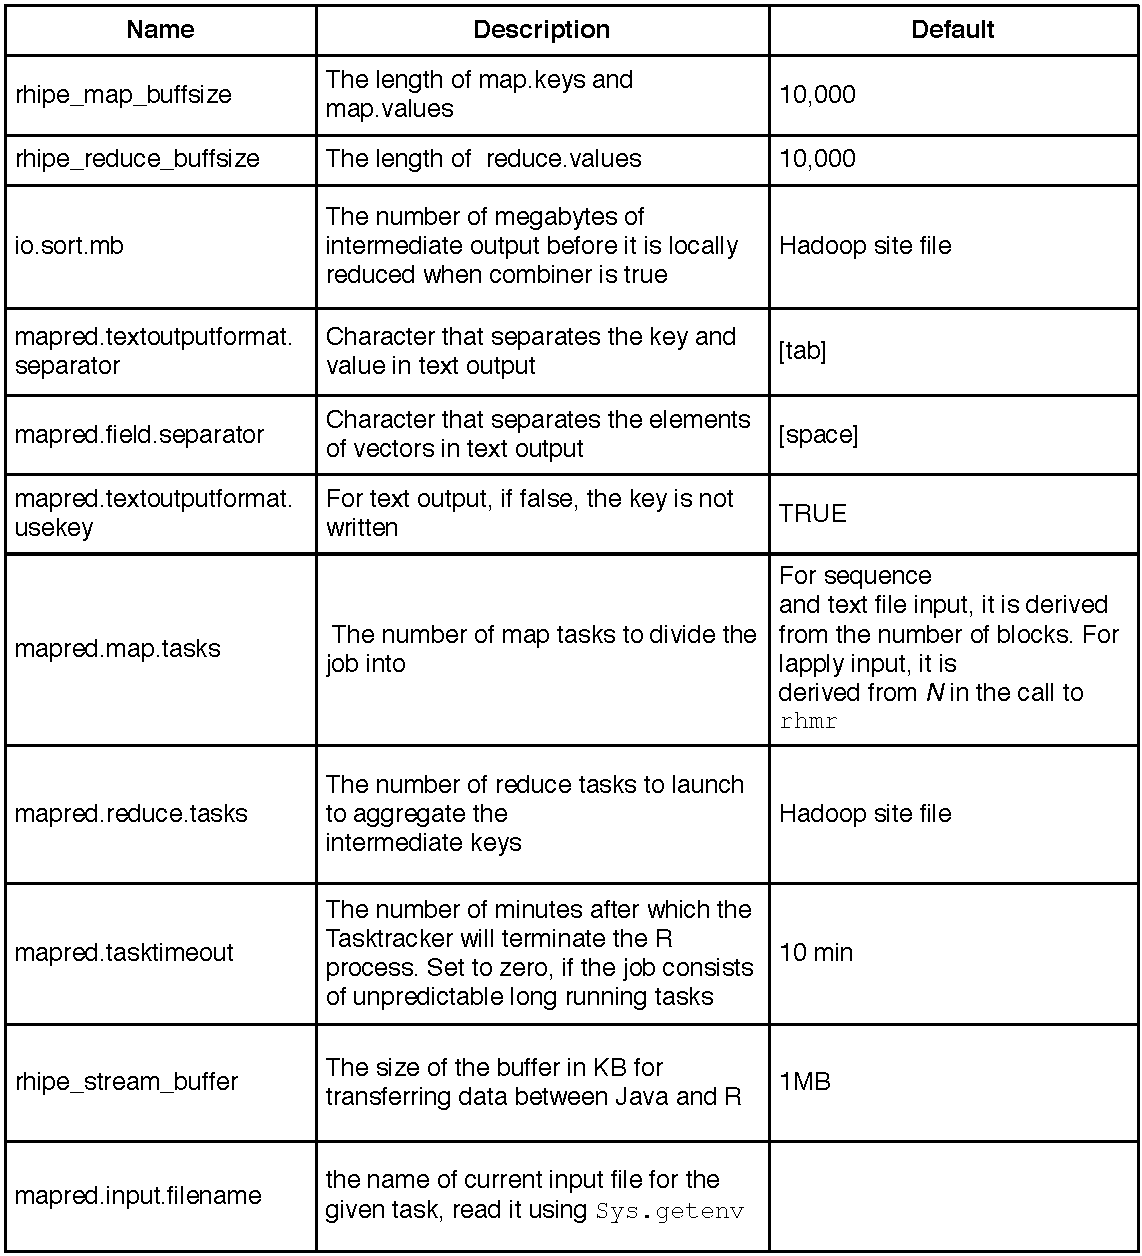
\includegraphics{tableopts.pdf}
\caption{Options useful for RHIPE and Hadoop}\end{figure}

\begin{thebibliography}{multicore}
\bibitem[STLa]{STLa}{\phantomsection\label{introduction:stla} 
Software and the concurrency revolution, H. Sutter  and J. Larus, \emph{ACM Queue, Volume 3,Number 7 2005}
}
\bibitem[MapRed]{MapRed}{\phantomsection\label{introduction:mapred} 
MapReduce: Simplified Data Processing on Large Clusters, Jeffrey Dean and Sanjay Ghemawat,*Communications of the ACM*, 2008
}
\bibitem[HynFan]{HynFan}{\phantomsection\label{introduction:hynfan} 
Hyndman, R. J. and Fan, Y. (1996) `Sample quantiles in statistical packages', \emph{American Statistician}, \emph{50}, 361-365).
}
\bibitem[SAS]{SAS}{\phantomsection\label{airline:sas} 
Congestion in the Sky: Vizualising Domestic Airline Traffic with SAS, Rick Wicklin and Robert Allison, \emph{SAS Institute}. \href{http://stat-computing.org/dataexpo/2009/posters/wicklin-allison.pdf}{http://stat-computing.org/dataexpo/2009/posters/wicklin-allison.pdf}
}
\bibitem[FLUSA]{FLUSA}{\phantomsection\label{airline:flusa} 
Delayed, Cancelled, On-Time, Boarding ... Flying in the USA, Heike  Hofmann, Di Cook, Chris Kielion, Barret Schloerke, Jon Hobbs, Adam Loy,Lawrence Mosley, David Rockoff, Yuanyuan Sun, Danielle Wrolstad and Tengfei. Yin, \emph{Iowa State University}, \href{http://stat-computing.org/dataexpo/2009/posters/hofmann-cook.pdf}{http://stat-computing.org/dataexpo/2009/posters/hofmann-cook.pdf}
}
\bibitem[ecuyer]{ecuyer}{\phantomsection\label{simulate:ecuyer} 
rstream: Streams of Random Numbers for Stochastic Simulation,Pierre L'Ecuyer and Josef Leydold, \href{http://cran.r-project.org/web/packages/rstream/index.html}{http://cran.r-project.org/web/packages/rstream/index.html}
}
\bibitem[Masac]{Masac}{\phantomsection\label{simulate:masac} 
Algorithm 806: SPRNG: A Scalable Library for Pseudorandom Number Generation, M. Mascagni and A. Srinivasan, \emph{ACM Transactions on Mathematical Software}, pages 436-461,volume 26, 2000
}
\bibitem[multicore]{multicore}{\phantomsection\label{functions:multicore} 
\href{http://http://cran.r-project.org/web/packages/multicore/index.html}{http://http://cran.r-project.org/web/packages/multicore/index.html}
}
\end{thebibliography}



\renewcommand{\indexname}{Index}
\printindex
\end{document}
